%% LyX 1.5.5 created this file.  For more info, see http://www.lyx.org/.
%% Do not edit unless you really know what you are doing.
\documentclass[a4paper,czech,czech,openright,cleardoubleempty,BCOR10mm,DIV11]{scrreprt}
\usepackage[T1]{fontenc}
\usepackage[utf8]{inputenc}
\usepackage{array}
\usepackage{longtable}
\usepackage{varioref}
\usepackage{wrapfig}
\usepackage{fancybox}
\usepackage{calc}
\usepackage{framed}
\usepackage{url}
\usepackage{graphicx}
\usepackage{color}
\usepackage{float}
\usepackage{svg}
\usepackage{amsmath}
\usepackage{makecell}
\usepackage{fourier} 
\usepackage{pdfpages}

\makeatletter

%%%%%%%%%%%%%%%%%%%%%%%%%%%%%% LyX specific LaTeX coěmmands.
\providecommand{\LyX}{L\kern-.1667em\lower.25em\hbox{Y}\kern-.125emX\@}
\newcommand{\lyxline}[1][1pt]{%
  \par\noindent%
  \rule[.5ex]{\linewidth}{#1}\par}
\newcommand{\noun}[1]{\textsc{#1}}
%% Special footnote code from the package 'stblftnt.sty'
%% Author: Robin Fairbairns -- Last revised Dec 13 1996
\let\SF@@footnote\footnote
\def\footnote{\ifx\protect\@typeset@protect
    \expandafter\SF@@footnote
  \else
    \expandafter\SF@gobble@opt
  \fi
}

\expandafter\def\csname SF@gobble@opt \endcsname{\@ifnextchar[%]
  \SF@gobble@twobracket
  \@gobble
}
\edef\SF@gobble@opt{\noexpand\protect
  \expandafter\noexpand\csname SF@gobble@opt \endcsname}
\def\SF@gobble@twobracket[#1]#2{}
%% Because html converters don't know tabularnewline
\providecommand{\tabularnewline}{\\}

%%%%%%%%%%%%%%%%%%%%%%%%%%%%%% Textclass specific LaTeX commands.
\newenvironment{lyxcode}
{\begin{list}{}{
\setlength{\rightmargin}{\leftmargin}
\setlength{\listparindent}{0pt}% needed for AMS classes
\raggedright
\setlength{\itemsep}{0pt}
\setlength{\parsep}{0pt}
\normalfont\ttfamily}%
 \item[]}
{\end{list}}

%%%%%%%%%%%%%%%%%%%%%%%%%%%%%% User specified LaTeX commands.
%<-------------------------------společná nastavení------------------------------>
\usepackage[czech]{babel}%počeštění názvů (Obsah, Kapitola, Literatura atp.)
\usepackage[]{hyperref} %odkazy v  pdf jsou klikací s barevnými rámečky
\usepackage[numbers,sort&compress]{natbib} %balíček pro citace literatury  
\usepackage{hypernat}%interakce mezi hyperref a natbib
\newcommand{\BibTeX}{{\sc Bib}\TeX}%BibTeX logo
\hypersetup{   % Nastavení polí PDF dokumentu 
pdftitle={Evaluation of Container-based Virtualization for standard company environment},%   
pdfauthor={Jan Cach},%  
pdfsubject={},%   
pdfkeywords={Cloud computing, Cloud native, Multi cloud, Kubernetes}%                             
}
\usepackage{multicol}




%<-----------------------------volání stylů----------------------------------------->
% (znak % je označení komentáře: co je za ním, není aktivní)
%<------------------------------------písmo----------------------------------------->
%\usepackage{packages/bc-latinmodern}
%\usepackage{packages/bc-times}
\usepackage{packages/bc-palatino}
%\usepackage{packages/bc-iwona}
%\usepackage{packages/bc-helvetika}


%<------------------------------záhlaví stránek------------------------------------>
%\usepackage{packages/bc-headings}
\usepackage{packages/bc-fancyhdr}

%<------------------------------hlavičky kapitol------------------------------------>
%\usepackage{packages/bc-neueskapitel}
%\usepackage{packages/bc-fancychap}

\makeatother

\usepackage{babel}

%java code block%

\usepackage{listings}
\usepackage{color}

\definecolor{dkgreen}{rgb}{0,0.6,0}
\definecolor{gray}{rgb}{0.5,0.5,0.5}
\definecolor{mauve}{rgb}{0.58,0,0.82}

% syntax highlight pro jazyk Javascript %
\definecolor{purple}{rgb}{0.65, 0.12, 0.82}
\lstdefinelanguage{JavaScript}{
  keywords={break, case, catch, const, continue, debugger, default, delete, do, else, false, finally, for, function, if, in, instanceof, let, new, null, return, switch, static, this, throw, true, try, typeof, var, void, while, with},
  morecomment=[l]{//},
  morecomment=[s]{/*}{*/},
  morestring=[b]',
  morestring=[b]",
  ndkeywords={class, constructor, export, extends, boolean, throw, implements, import},
  keywordstyle=\color{blue}\bfseries,
  ndkeywordstyle=\color{gray}\bfseries,
  identifierstyle=\color{black},
  commentstyle=\color{purple}\ttfamily,
  stringstyle=\color{red}\ttfamily,
  sensitive=true
}

\lstset{,
  language=Javascript,
  aboveskip=3mm,
  belowskip=3mm,
  showstringspaces=false,
  columns=flexible,
  inputencoding=utf8,
    extendedchars=true,
    literate=%
    {á}{{\'a}}1
    {č}{{\v{c}}}1
    {ď}{{\v{d}}}1
    {é}{{\'e}}1
    {ě}{{\v{e}}}1
    {í}{{\'i}}1
    {ň}{{\v{n}}}1
    {ó}{{\'o}}1
    {ř}{{\v{r}}}1
    {š}{{\v{s}}}1
    {ť}{{\v{t}}}1
    {ú}{{\'u}}1
    {ů}{{\r{u}}}1
    {ý}{{\'y}}1
    {ž}{{\v{z}}}1
    {Á}{{\'A}}1
    {Č}{{\v{C}}}1
    {Ď}{{\v{D}}}1
    {É}{{\'E}}1
    {Ě}{{\v{E}}}1
    {Í}{{\'I}}1
    {Ň}{{\v{N}}}1
    {Ó}{{\'O}}1
    {Ř}{{\v{R}}}1
    {Š}{{\v{S}}}1
    {Ť}{{\v{T}}}1
    {Ú}{{\'U}}1
    {Ů}{{\r{U}}}1
    {Ý}{{\'Y}}1
    {Ž}{{\v{Z}}}1,
  basicstyle={\small\ttfamily},
  xleftmargin=1cm,
  keywordstyle=\color{blue},
  commentstyle=\color{dkgreen},
  stringstyle=\color{mauve},
  breaklines=true,
  breakatwhitespace=true,
  tabsize=3
}
\usepackage{url}
\makeatletter
\g@addto@macro{\UrlBreaks}{\UrlOrds}
\makeatother

% vlastni package
\usepackage{placeins}
\usepackage{multirow}
\usepackage{pdfpages}
% fonty popisku
\usepackage[font=small,labelfont=bf]{caption}
% radkovani 
\renewcommand{\baselinestretch}{1.2}
\renewcommand*{\lstlistingname}{Kód} %prejmenovani lstlisting
\renewcommand*{\lstlistlistingname}{Seznam ukázek kódu}
\renewcommand*{\figurename}{Obrázek} %prejmenovani figure
\renewcommand*{\listfigurename}{Seznam obrázků}
\renewcommand*{\bibname}{Literatura} %prejmenovani figure
\renewcommand{\tablename}{Tabulka}
\renewcommand{\listtablename}{Seznam tabulek}
\renewcommand{\contentsname}{Obsah}
% vlastni styly tabulek
\newcolumntype{C}[1]{>{\centering\arraybackslash}m{#1}}
\begin{document}

\cleardoublepage{}~\thispagestyle{empty}\begin{center}\pagenumbering{roman}\vspace{10mm}


\textsf{\textsc{\noun{\LARGE Univerzita Hradec Králové}}}\\
\vspace{0.5em}
\textsc{\noun{\LARGE Fakulta informatiky a managementu}}\\
\vspace*{1em}
\textsf{\textsc{\noun{\Large katedra informačních technologií }}}


%%% Aby vložení loga  správně fungovalo, je třeba mít soubor uhk.png nahraný v adresáři logo,
%%% tj. v adresáři, kde se nachází překládaný zdrojový soubor. 
\vspace{4cm}

\textsf{\huge DIPLOMOVÁ PRÁCE}{\huge \par}

\vspace{15mm}


\textsf{\LARGE Implementace hybridního multi-cloud konceptu pro běh distribuovaných aplikací v kontejnerech a virtuálních serverech do enterprise prostředí}{\LARGE \par}

\vspace{10mm}


\end{center} 

\vspace*{\fill}


\vspace{10mm}


\begin{description}
%studijni obor???
\item [{{\large Autor:}}] \noindent \textsf{\large Jan Cach}{\large \par}
\item [{{\large Studijní obor:}}] \noindent \textsf{\large Aplikovaná informatika}{\large \par}
\item [{{\large Vedoucí~práce:}}] \noindent \textsf{\large Ing. Jakub Pavlík, MSc.}{\large \hfill{}}\textsf{\large Hradec Králové, 2019}{\large{}
% doplňte rok vzniku vaší bakalářské práce
}{\large \par}
\end{description}

\clearpage{}
~\thispagestyle{empty}{\small ~\vfill{}
}{\small \par}

\noindent {\small \vfill{}
 % nastavuje dynamické umístění následujícího textu do spodní části stránky
~}{\small \par}

\noindent {\small Prohlašuji, že jsem diplomonou práci vypracoval samostatně a uvedl jsem všechny použité prameny a literaturu.}{\small \par}

{\small \bigskip{}
}\noindent {\small{} V Hradci Králové dne \today\hspace{\fill}Jan Cach}\\
{\small{} % doplňte patřičné datum, jméno a příjmení
}{\small \par}

{\small %%%   Výtisk pak na tomto míste nezapomeňte PODEPSAT!
%%%                                         *********
}{\small \par}

\clearpage{}
~\thispagestyle{empty}{\small ~\vfill{}
}{\small \par}

\noindent {\small Rád bych poděkoval Ing. Jakubu Pavlíkovi, MSc. za odborné vedení práce, podnětné rady a čas, který mi věnoval. Dále bych chtěl poděkovat své rodině za podporu při tvorbě této práce. \newpage{}}{\small \par}
\clearpage{}
~\thispagestyle{empty}{\small ~\vfill{}
}{\small \par}
\noindent {\small \vfill{}
 % nastavuje dynamické umístění následujícího textu do spodní části stránky
~}{\small \par}
\section*{Anotace}
Tato diplomová práce se zaměřuje na problematiku Cloud-Native aplikací a infrastruktury společně s jejím využitím v hybridním multi-cloud prostředí. Cloud-Native je stále se rozvíjející oblast, jejíž snahou je vytváření a správa aplikací, které naplno využívají potenciálu cloudových platforem. Tento přístup pokrývá celý životní cyklus aplikace, který zahrnuje architekturu aplikace, její nasazení, správu a monitoring. Cílem této práce je analyzovat a navrhnout platformu, která bude umožňovat běh distribuovaných aplikací v prostředí multi-cloudu. V praktické části je tato navržená platforma \linebreak implementována a otestována na vybraných scénářích.
\subsubsection*{Klíčová slova}
Cloud computing, Cloud native, Multi cloud, Kubernetes

\section*{Annotation}
Title: Implementation of hybrid multi-cloud concept for distributed aplications accros containers and VMs into enterprise environment
\vspace{0.5cm}\FloatBarrier
This master thesis focuses on Cloud-Native applications and infrastructure \linebreak problematics together with its utilization in hybrid multi-cloud environment. Cloud-Native is dynamic domain. Its goal is the creation and management of applications, which utilize all benefits of cloud platforms. This approach covers whole application life cycle, which includes application architecture, deployment, management and \linebreak monitoring. The main goal of this thesis is to analyze and design platform, which will \linebreak allow distributed applications to be run in the hybrid multi-cloud environment. This platform is implemented and tested with selected scenarios in the hands-on part.
\subsubsection*{Key words}
Cloud computing, Cloud native, Multi cloud, Kubernetes

\noindent {\small ~\vfill{}
}{\small \par}

\cleardoublepage{}\thispagestyle{empty}{\small \tableofcontents{}% vkládá automaticky generovaný obsah dokumentu
\cleardoublepage{}}{\small \par}

\chapter{Úvod}
\pagenumbering{arabic}
\setcounter{page}{1}
V současné době dochází na poli návrhu a vývoje počítačových systémů k výraznému posunu. Příchod cloud computingu a později cloud native přístupu transformoval základní principy návrhu a běhu aplikací. Namísto fyzické infrastruktury, vývojáři implementují služby nad sofistikovanou virtualizovanou platformou, která přináší výhody oproti klasickému přístupu. První generace systémů, které běželi v cloudovém \linebreak prostředí se nazývaly “cloud enabled” systémy. Tyto systémy, typické pro cloud computing éru, byly přeneseny do prostředí cloudu, ale byly provozovány velice podobně jako v období před cloud computingem. Z tohoto důvodu aplikace plně nevyužívaly výhody, které jim cloud computing nabízel. Pro překonání těchto problémů se vytvořily nové přístupy a technologie v tvorbě aplikací, souhrně nazývané cloud native \cite{hotcloud}. 
\par
    Cloud native přístup k tvorbě a správě aplikací zasahuje do celého životního cyklu aplikace. Architektura cloud native aplikací je založena na mikroslužbách, které \newline rozdělují aplikace na menší vzájemně nezávislé celky. Tyto celky se lépe rozšiřují, udržují a škálují oproti monolitickým aplikacím. Dalším stavebním blokem cloud native přístupu jsou kontejnery. Kontejnery v sobě zapouzdřují závislosti aplikací a \newline napomáhají přenositelnosti aplikací mezi testovacím a produkčním prostředím. Pro správu cloud native aplikací jsou používány orchestrátory kontejnerů, které přináší jednoduchou a automatizovanou práci s kontejnery. 
	\par
        Cloud native přístup má více oblastí použití. První oblastí jsou aplikace, které \linebreak vyžadují vysokou dostupnost a škálovatelnost. Vysoké dostupnosti může být dosaženo s využitím orchestrátorů kontejnerů, které sledují stav jednotlivých mikroslužeb a v případě výpadku jsou schopné nahradit chybné kontejnery. Architektura mikroslužeb dovoluje škálovat pouze potřebnou část aplikace. S rozvojem Internetu věcí (IoT) se cloud native přístup prosazuje i v prostředí Edge computingu. Cílem Edge computingu je zpracovávat data, co nejblíže k jejich zdroji a umožnit tak jejich rychlé zpracovaní a snížení doby odezvy. Stejná situace panuje i v prostředí multi-cloud. Společnosti mají zájem jednotně spravovat zdroje a využívat služby napříč více poskytovateli cloudových služeb. Společnosti jako Google, Amazon, Red Hat a spousta dalších se snaží přijít s vlastním řešením, které nabídne jednotnou správu zdrojů a aplikací. Z těchto důvodů se tato oblast stále rozvíjí a nabízí tak prostor pro nové technologie.
	\par
	    Cílem této diplomové práce je analyzovat a navrhnout platformu, která bude umožňovat běh distribuovaných aplikací v prostředí multi-cloudu. Řešení práce spočívá ve vytvoření požadavků pro takovou platformu, navrhnutí architektury dané platformy a vytvoření prototypu systému, který bude společně s jejím testováním výstupem této práce. 
	    \par
	        Diplomová práce se v teoretické části zaměřuje na vývoj cloud computingu. V první kapitole je popsaný princip cloud computing. Druhá kapitola navazuje na cloud computing a představuje cloud native computing jako nové cloudové paradigma. V kapitole jsou představeny základní principy a technologie cloud native computingu a v čem se odlišuje od předchozího přístupu. Kapitola dále představuje oblasti využití cloud native přistupu v podobě edge cloudu a hybrid cloudu. V podkapitole hybrid cloud jsou dále rozebrány existující nástroje pro tuto oblast. Poznatky z teoretické části jsou dále využity pro definici požadavků na aplikaci, která umožní běh distribuovaných aplikací. Praktická část práce se dále zabývá návrhem takového systému a implementací prototypu. V poslední části práce jsou uvedeny výsledky z testování vytvořené aplikace, které mají za ukol ověřit funkčnost navržené aplikace. 


\chapter{Úvod}
\pagenumbering{arabic}
\setcounter{page}{1}
\section{Směr Cloud Computingu}
Označení Cloud computing je některými odborníky považováno za nové paradigma, někteří dokonce mluví o nové technologii, která umožňuje přístup k výpočetním zdrojům a službám přes internet \cite{bohm2010cloud}. Cloud computing, často označovaný pouze jako cloud, tak dovoluje jednotlivcům, malým firmám a dalším subjektům jednoduchý přístup k výpočetnímu výkonu z pohodlí domova či kanceláře za přijatelnou cenu, bez nutnosti spravovat celou výpočetní infrastrukturu. Uživatelé jsou tak odstíněni od konfigurace serverů a síťových zařízení a služeb samotných. \newline
Podle \cite{cc2011principles} lze na Cloud computing nahlížet jako na využívání elektřiny. Elektřinu využíváme jako službu. Nezajímáme se o to jak se elektřina vyrábí a jak je dodávána do jednotlivých elektrických zásuvek v našem pokoji. My pouze připojíme zařízení do elektrické zásuvky a očekáváme, že například nabije náš telefon či počítač. Pokud tento příklad přeneseme do oblasti IT, znamená to, že uživatelé jsou odstínění od vnitřního fungování nějaké služby nebo použitých technologiích. Jako příklad může být brána služba cloudového uložiště fotografií. Pro uživatele je důležité, že si může fotografie prohlížet  z různých zařízení přes internet odkudkoliv a kdykoliv. Ostatní problémy jako jsou uložení a záloha těchto dat, webové rozhraní pro práci s fotografiemi a další je ponecháno na poskytovateli služby. \newline
Některé instituce, akademičtí pracovníci či IT inženýři vytvořili definice a charakteristiky  popisující Cloud computing. Například Americký národní institut standardů a technologií (NIST) \cite{mel2011nist}, definuje cloud computing následovně:
Cloud computing je model pro pohodlný síťový přístup ke skupině konfigurovatelných výpočetních zdrojů, jako jsou počítačové sítě, servery, datová uložiště, aplikace a služby, které jsou dostupné odkudkoliv a okamžitě na vyžádání. Tyto zdroje mohou být rychle vytvořeny a uvolněny  s vyvinutím minimálního úsilí nebo minimální interakce od provozovatele dané služby. \newline 
Definice ze zdroje \cite{Vaquero-cloud-definition} zmiňuje, že uživatelé platí pouze za zdroje, které skutečně využívají podle sjednaných podmínek. Tento postup se nazývá pay-per-use model. Znamená to žádné pevně stanovené poplatky bez ohledu na to zda zákazník využívá polovinu přidělených zdrojů nebo se využití zdrojů blíží 100 \%. Díky tomu je možné si například vypočítat náklady na provozování služby u různých firem a rozhodnout se tak pro nejvhodnější platformu. \newline
    Armbrust a jeho kolegové z Kalifornské Univerzity v Berkeley \cite{Ambrust2009}, shrnují cloud computing do 3 bodů. Prvním bodem je zdání, že uživatel má k dispozici nekonečný objem výpočetních zdrojů. Z tohoto důvodu není potřeba dopředu plánovat zda bude k dispozici dostatek zdrojů, zdroje jsou dynamicky přidávány a odebírány na požádání. Druhým bodem je skutečnost, že není potřebné uzavírat žádné předběžné závazky ze strany uživatele. Toto dovoluje firmám začít s malým počtem zdrojů a postupně navyšovat zdroje s rostoucími potřebami. Třetím a posledním bodem je zde platit za využívané zdroje ve velice krátkém horizontu, např. hodin nebo dní a poté je uvolnit podle potřeb.

\section{Servisní modely cloud computingu}
Cloud computing můžeme rozdělit do tří kategorií podle služeb, která má daný model poskytovat. Zmíněnými modely jsou Infrasracture as a service (IaaS), Platform as a service (PaaS) a Software as a service (SaaS). Jednotlivé modely se liší ve využítí a účelu pro jaký si je společnost pořizuje. V následujích odstavcích jsou jednotlivé modely blíže představeny. 

\subsection{Infrastructure as a Service}
Z obrázku \cite{cloud-computing-service-model} vyplývá, že IaaS je základem cloudu a nachází se v nejnižší vrstvě celého cloud stacku. Zákazník dostává k dispozici infrastruktu a vše co se nachází nad infrastrukturou jako jsou data, databáze, aplikace a prostředí pro běh aplikací si zákazník ovládá a spravuje sám. Poskytovatel infrastruktury je zodpovědný za fyzické servery, networking, storage a virtualizační vrstvu zajištující vytváření, mazání a správu virtuálních serverů pro lepší využití zdrojů. To znamená, že poskytovatel spravuje fyzické servery včetně disků, pamětí a zdrojů. Dále obstarává konektivitu mezi servery, spravuje switche a routery. Poskytovatel také monitoruje infrastrukturu aby mohl vhodně a včas reagovat na nastalé problémy.\newline
Dostupnost těchto služeb nebo čas do kterého musí poskytovatel adekvátně zareagovat je definována pomocí SLA smlouvy, která je sjednána mezi poskytovatelem služby a zákazníkem \cite{Rongdong}.
Jednotlivé zdroje jako jsou servery, uložiště atd. jsou většinou rozděleny do  menších skupin které jsou poté přiděleny různým uživatelům podle jejich potřeb. Takovými uživateli mohou být například různé firmy nebo rozdílné vývojové týmy v rámci jedné společnosti. Tento způsob vede k lepší správě a využití zdrojů. Uživatelé mají přehled o aktuálním vytížení, kapacitě jednotlivých zdrojů, díky čemuž mohou plánovat případné navýšení kapacity uložiště nebo RAM.\newline
    Výhodou pro uživatele je, že nemusí vlastnit datacentrum se servery, chlazením, monitoringem a dalšími technologiemi, které jsou velice nákladné na pořízení a správu. Nemusí také řešit nákup hardwaru, výměnu starých nebo vadných kusů atd. Zákazníci využívající IaaS nemusí mít odborníky na  problematiku infrastruktury. Všechny tyto aspekty šetří pořizovací i provozní náklady. Při modelu pay-per-use firmy platí pouze za zdroje které využívají a pouze po dobu jakou je využívají. Další výhodou je flexibilita. Uživatelé mají možnost dynamicky přidávat a odebírat zdroje a pružně tak reagovat na velké vytížení, případně šetřit zdroje a peníze při malém vytížení. Zákazníci musí zvážit rizika spojená s bezpečností a důkladně si zjistit podmínky týkající se ztráty nebo odcizení dat, protože data jsou uložena v uložišti, které nejsou ve vlastnictví zákazníka stejně tak tok dat skze sít.\newline
    Mezi společnosti, které nabízejí IaaS patří AWS EC2 (Amazon elastic cloud computing), nebo společnost BlueLock  \cite{salah2011performance}. IaaS řešení poskytuje i Google s nástrojem Google Compute Engine. Dalším významným řešením je open source produkt OpenStack. Jedná se o komunitní projekt a  mnoho společností aktivně přispívá do tohoto projektu. Existuje mnoho společností, které nabízejí svou upravenou verzi OpenStacku \cite{singh2014critical}.

\subsection{Platform as a Service}
    Platform as a service, zkráceně PaaS, je vývojářská platforma podporující plnohodnotný životní cyklus aplikace. PaaS umožňuje uživatelům cloudu vyvíjet cloudové služby a aplikace přímo v prostředí PaaS cloudu \cite{dilon2010cloud}.\newline
         V PaaS modelu poskytování služeb je uživatel zodpovědný pouze za aplikaci a data, se kterými tato aplikace pracuje, proto je používání PaaS pro programátory jednodušší a rychlejší oproti IaaS řešení. Poskytovatel služby má, na rozdíl od IaaS, na starost správu databází, vytváření runtime prostředí pro aplikace nebo provoz webového serveru. Cloud provider poskytuje různé další služby jako jsou verzovací systém nebo lifecycle management aplikace a dále také integrace s různým softwarem třetích stran. Uživatel si nejčastěji vybírá z katalogu jakou databázi bude chtít používat a také runtime prostředí pro programovací jazyk jaký chce uživatel pro vývoj aplikace využít. Výběr jednotlivých zdrojů se liší v závislosti na poskytovateli. Uživatel si jednoduše přes webové rozhraní nebo CLI nástroj vytváří a přidává zdroje které chce využívat. Vše je otázkou několika málo kliknutí. Tento způsob urychluje vývoj aplikace a nenutí programátory učit se konfigurovat různé služby a oni se tak mohou plně věnovat vývoji aplikace.\newline
	      Poskytovatelé služby zjednodušují vývojářům celý proces vývoje aplikace přes správu kódu, nasazení a otestování aplikace, nasazení aplikace do produkce a její další růst, vývoj a monitoring v přehledných grafech a tabulkách. Vývojáři publikují kód do verzovacího systému. Odtud může být pomocí testovacích nástrojů poskytovatelů aplikace nasazena do testovacího provozu a dále po odsouhlasení nasazena do produkce. Poskytovatelé PaaS služeb takto přidávají prvky CI/CD a představují  moderním přístup k tvorbě aplikací.\newline 
	      Další službu, kterou PaaS poskytovatelé nabízí je automatické škálování aplikace. Uživatelé jsou odstíněni od manuálního nastavování loadbalancerů a přidávání dalších webových či databázových serverů. Přidávání serverů pro lepší rozdělení zátěže probíhá automaticky podle předem definovaných pravidel podle toho jak se aplikace rozrůstá. Stejně jako IaaS i PaaS využívá modelu pay-per-use, tedy uživatelé platí pouze za zdroje, které využívají. Jako nevýhodu PaaS řešení může být omezená podpora programovacích jazyků. Každý provozovatel platformy podporuje rozdílné programovací jazyky. Uživatelé jsou tak nuceni vytvořit aplikaci  v jednom z podporovaných jazyků, případně vybrat jiného poskytovatele, který daný jazyk podporuje. Jiný provozovatel může nabízet jiné služby za jiných podmínek. Z tohoto důvodu je nutné dopředu zvážit výběr poskytovatele PaaS služby, protože není snadné a bezbolestné migrovat aplikace mezi různými providery.\newline 
	      Srovnáním PaaS poskytovatelů v práci \cite{lucassen2013ecosystem}, bylo zjištěno že ve sledovaných aspektech si nejlépe vedlo Heroku, následované řešením od společnosti RedHat a dále Azure od firmy Microsoft. Mezi srovávanými služby byly také Google AppEngine, řešení od CloudFoundry a nebo služba poskytovaná firmou dotCloud. Mezi sledovanými aspekty byli například aktivní vývojáři, kteří na dané platformě vyvíjeli za poslední rok nebo počet různých programovacích jazyků provozovaných na dané platformě. Ze závěrů se dá usoudit, že uvedení poskytovatelé PaaS služby pokrývají téměř 100\% trhu.

\subsection{Software as a Service}
Software as a service, zkráceně SaaS, je určen pro koncové uživatele. Poskytovatel Saas spravuje vše od aplikace přes uložení dat až po servery na kterých aplikace běží, tedy celou infrastrukturu i životní cyklus aplikace.  Uživateli stačí se skrze webový prohlížeč, mobilní telefon či jiné zařízení, k aplikaci přihlásit a začít ji používat.
Doručování aplikace jako služby přináší uživatelům nové možnosti jak zrychlit a zkvalitnit práci s nižšími náklady. Pokud si uživatel nějakou službu vybere je otázkou hodiny, než může aplikaci začít používat. Tento proces zahrnuje vytvoření organizace, přidání uživatelů a jejich práv a poté je možné začít aplikaci používat. Tento proces je velmi rychlý oproti klasickému nasazení na servery vlastněné uživatelem. Nevýhodou může být pokud vybraná služba neumožňuje integraci s firemním systémem pro správu uživatelů a jejich práv. Další výhodou oproti desktopové aplikaci je možnost přístupu k aplikaci a jejím datům z různých zařízení a různých lokalit. Většinou stačí uživateli internet pro přístup k aplikaci a není tak vázaný pouze na firemní počítač umístěný v budově firmy.\newline
Velkým plusem SaaS řešení je jasná a dopředu určená cena za využívání dané služby. Poskytovatelé na svých stránkách poskytují kompletní ceník. Uživatel si tak může spočítat a porovnat, které řešení je nejvýhodnější. Změnila se také licenční politika. Například cena služby není vypočítávána podle počtu jader procesoru serveru na kterém je aplikace nasazena, ale podle počtu uživatelů, kteří aplikaci používají. Poskytovatelé dále nabízejí dynamické přidávání a odebírání uživatelů. Přidání zaměstnance do aplikace je opět otázkou minut, stejně jako jeho odebrání. Stejně jako u předchozích typů služeb i zde platí uživatel pouze za to co používá. Šetří tak náklady na IT profesionály a infrastrukturu. Z tohoto důvodu se aplikace stávají více dostupné i malým a středním podnikům, které nemusejí platit infrastrukturu a odborníky, kteří se o ni starají.\newline 
Další významnou složkou pro poskytovatele i uživatele je nasazení nových verzí aplikace a také bezpečnostní aktualizace. Uživatelé běžně dostávají nejnovější verzi aplikace bez nutnosti cokoliv aktualizovat nebo instalovat na svém zařízení. Poskytovatel na druhé straně, může po otestování nové verze aplikace uživatele přesměrovat na novou verzi.\newline 
Společnosti mohou využívat různé druhy aplikací jako jsou aplikace pro řízení vztahů se zákazníkem, kancelářské nástroje, účetní programy a mnoho dalších. První společnost, která nabízela SaaS byla společnost SalesForce, nabízející jejich CRM řešení \cite{salesforce2018}. Dalšími aplikacemi jsou balík nejenom kancelářských aplikací Google Apps, uložiště dat DropBox a také komunikační nástroj Slack.



\chapter{Cloud-Native infrastruktura a aplikace}
Cloud native strategii můžeme považovat za nástupce cloud computingu. Cílem cloud native není pouze běh aplikací v prostředí cloudu, ale zaměřuje se na celý životní cyklus aplikace od architektury aplikace, nasazení aplikace, škálovatelnost, doručování nových verzí a také monitoring aplikace a statistiky používání. Tento přístup by měl umožňovat správu velkých a komplexních aplikací, které jsou ovšem přizpůsobené prostředí cloudu a využívají možnosti, které cloud nabízí. Součástí Cloud native je také přechod od velkých monolitických aplikací na menší microservice. Monolitické aplikace byly často migrovány do cloudového prostředí pouze jako monolitické virtuální servery. Takováto aplikace není odolná vůči výpadkům v dostupnosti a  také nárokům na škálovatelnost \cite{BRUNNER} a nevyužívá tak plně možností které prostředí cloudu nabízí. Cloud native přístup se snaží všechny tyto nevýhody odstranit. \par
    S vývojem cloud computingu se měnil i pohled na servery (fyzické servery, virtuální servery nebo kontejnery) a jejich správu. Podle analogie s Pets and Cattle \cite{petsvscattle} pokud vidíme server jako něco, co může být kdykoliv zničeno a nahrazeno, potom mluvime o stádu. Pokud vidíme server jako nepostradatelný, tedy jeho ztráta by byla kritická poté mluvíme o mazlíčkovi (Pet). Pokud se podíváme na tuto zvířecí analogii blíže, za pets, neboli mazlíčky považujeme servery, které jsou v naší infrastruktuře nepostradatelné nebo to jsou unikátní systémy, které musí vždy fungovat. Takovéto servery jsou manuálně nakonfigurovány a spravovány, z toho důvodu o ně nechceme přijít a děláme vše pro to aby nepřestaly fungovat. Do této skupiny patří mainframy, loadbalancery, firewally a také master-slave databázové systémy.  Na druhé straně máme servery, které jsou vytvořeny pomocí nástrojů pro automatizaci. Pokud jeden nebo více serverů přestane fungovat, můžeme je nahradit novými servery se stejnou konfigurací. Zde již není potřeba starat se o každý server samostatně, pokud nastane problém server je restartován nebo nahraze novým serverem. Sem můžeme zařadit webové servery případně clustrované databáze. V tomto případě máme například více webových serverů, pokud jeden vypadne ostatní převezmou kontrolu. Poškozený server je poté nahrazen nově vytvořeným webovým serverem se stejnou konfigurací. \par
        Podle Cloud native computing foundation (CNCF) dovoluje cloud native přístup organizacím vytvářet a provozovat škálovatelné aplikace v moderním a dynamickém prostředí jako je public, private nebo hybrid cloud. Technologie jako jsou kontejnery, service meshes, microservices, neměnné infrastruktury a deklarativní API ilustrují cloud native přístup. Tyto techniky umožňují volně provázané systémy, které jsou flexibilní, spravovatelné a dají se monitorovat. V kombinaci se solidní automatizací dovolují vývojářům dělat předvídatelné, velké a časté změny s minimální námahou \cite{CNCFdefinition}. \par
	CNCF je organizace, která se snaží definovat a sjednocovat cloud native standardy a zastřešovat jednotlivé open source technologie celého cloud stacku. To znamená, že zde nalezneme technologie runtime kontejnerů, nástroje pro orchestraci kontejnerů, technologie pro komunikaci mezi jednotlivými službami, bezpečnost, uložiště pro cloud native prostředí a nástroje pro logování a monitoring služeb. CNCF také podporuje komunitu okolo cloud native technologií a snaží se také podporovat spolupráci mezi vývojáři, koncovými uživateli a také mezi výrobci, kteří se mohou potkat a diskutovat nové technologie, trendy a postupy na pravidelných konferencích. Organizace také nabízí konzultace, tréninky a certifikace ať už jednotlivcům z řad vývojářů tak i zaměstnancům společností, kteří se mohou naučit pracovat s novými technologiemi a začít tyto nabyté znalosti uplatňovat v byznysu svých společností a šířit dále mezi své spolupracovníky. \par
	    Studie \cite{KRATZKE} se zabývá vysvětlením pojmu cloud native a jeho lepším porozuměním. Tato studie definuje cloud native aplikaci jako distribuovaný, flexibilní a horizontálně škálovatelný systém skládající se z microservices, které izolují stav aplikace v minimu stavových komponent. Aplikace a každá její část jsou navrženy podle vzorů zaměřených na prostředí cloudu na samoobslužné flexibilní platformě. \par
	        
\section{Stavební bloky cloud native aplikace}
		Pokud mají být cloud native aplikace dobře škálovatelné, rozšiřitelné a spravovatelné, potřebují být k tomuto účelu navrženy. S monolitickou architekturou není možné tyto požadavky naplno splnit. Cloud native přístup tak přichází s microservices architekturou, která rozděluje aplikaci na menší aplikace, které se lépe škálují, spravují a testují. Tato architektura je připravená plně využít všech možností prostředí cloudu. Jestliže dříve byli virtuální servery základní jednotkou nasazení aplikace do cloud prostředí, dnes v době cloud native aplikací jsou to kontejnery. Kontejnery jsou méně náročné na zdroje a startují rychleji v porovnání s virtuálními servery. Poskytují izolaci pro jednotlivé microservicy a jsou základním jednotkou nasazení. Jelikož má aplikace všechny potřebné závislosti zabalené uvnitř kontejneru je možné aplikace nasadit v jiném \linebreak prostředí bez komplikací. Dalším krokem je nasazení a správa aplikace. Pro tuto část se používají orchestrátory kontejnerů. Orchestrátory obstarávají spoustu věcí od spuštění jednotlivých kontejnerů, monitorování jejich stavu, doručování nových verzí přes komunikaci mezi kontejnery,load balancing, bezpečnost a řízení přístupu až po monitoring a další statistiky celé aplikace. Orchestrátory nabízejí možnost nahradit jednotlivé služby z předchozího výčtu jinou technologií pomocí pluginů. V následující části jsou detailně představeny jednotlivé technologie celého cloud native stacku.

\subsection{Architektura mikroslužeb}
Microservice architektura vznikla jako reakce na monolitické aplikace, které se s rostoucí velikostí aplikace, počtem uživatelů aplikace a komplexností celého systému staly hůře škálovatelné, spravovatelné, rozšiřitelné a testovatelné. Velké společnosti jako přepravní služba Uber \cite{uber}, online distributor hudby SoundCloud \cite{soundcloud}, společnost \linebreak Groupon zabývající se online obchodováním \cite{groupon} a také online distributor filmů a seriálů Netflix se rozhodli přejít od monolitické architektury na microservices architekturu a plně tak využít možností cloudu. Zmíněné společnosti se staly průkopníky v použití microservice architektury pro provozování aplikací a zároveň přinesly ostatním společnostem nové poznatky a technologie, které řeší problémy na které během vývoje narazily. Jedním z příkladů může být technologie ChaosMonkey vytvořená společností Neflix \cite{chaosmonkey}. Tato technologie náhodně vypíná produkční servery a kontejnery a simuluje tak výpadek služeb. Tento mechanismus nutí zaměstnance navrhovat a upravovat aplikace tak, aby takovéto výpadky bez následků přečkaly.\par
Microservices architektura je ze své podstaty protiklad monolitické aplikace. Microservice rozdělují aplikaci na menší celky, které spolupracují, aby dosáhly výsledné funkcionality. Monolitická aplikace je zase tvořena jako jeden velký celek. Pro nastínění pojmu monolitická aplikace můžeme například využít článek od pracovníků ze \linebreak společnosti Google \cite{googleMonolith}. Monolitická aplikace je doručena jako celek, například jeden WAR soubor v jazyce Java nebo .NET webová aplikace. Takové aplikace se obvykle skládají ze tří vrstev. První je databázová vrstva pro přístup k datům, dále vrstva logiky aplikace a prezentační vrstva zodpovědná za zobrazování dat uživatelům. Monolitické aplikace se drží objektově orientovaného přistupu, jsou komplexní a vykazují velkou vnitřní provázanost jednotlivých tříd systému. \par
Microservices je nová architektura cloud native aplikací navržená a optimalizovaná pro cloud, která zmíněné problémy řeší. Cloud native aplikace se skládají z malých služeb, které dohromady vykonávají funkcionalitu celého systému. Každá služba (microservice) vykonává pouze svou činnost, část logiky aplikace, pro kterou je určena a má definované API pomocí kterého mezi sebou jednotlivé služby komunikují \cite{balalaieMicroservies}. \par
    Rozdělení aplikace na jednotlivé menší jednotky, microservices, dělá aplikace lépe implementovatelné a srozumitelnější. Jednotlivé části aplikace jsou na sobě nezávislé, mají oddělené zdrojové kódy a mohou být napsané v rozdílných programovacích jazycích. Díky tomu je vývoj rychlejší, stejně jako nasazení nové verze dané microservice. Přidání či změna funkcionality neovlivňuje celý systém, ale pouze malou část systému. Jednotlivé služby mezi sebou komunikují pomocí definovaných API volání. Služba při volání na API ví jaká data musí poslat a jaká data má očekávat. Toho je dosaženo s využitím IDL nástrojů (Interface definition language). IDL dovoluje definovat nezávisle na použitém programovacím jazyku metody, které API nabízí, dále jaké parametry jednotlivá volání přijímají a jaký je formát odpovědi na dané API volání. IDL poté dovoluje vygenerování serverové části aplikace a klientské části aplikace pro libovolný podporovaný jazyk, které vychází z jednoho zdroje a jejich případná úprava se provádí pouze na jednom místě. Díky tomu jsou vyřešeny služby, které API nabízí a formát zpráv, které budou mezi klientem a serverem posílány. Mezi zástupce patří například Apache Thrift \cite{sleethrift} nebo Protocol buffers. \par
    V porovnání s monolitickou aplikací umožňuje microservice architektura rychlejší a častější doručování změn. Při změně jedné služby systému stačí pouze vytvořit a otestovat novou verzi změněné části. Na druhé straně změna v monolitické aplikaci vyžaduje vytvoření a otestování celého monolitu, což je časově náročnější a celý proces doručení záplat a nové funkcionality se časově prodlužuje. \par
    Dalším benefitem microservices architektury je škálovatelnost jednotlivých částí aplikace. Při velké zátěži se efektivně škáluje pouze vytěžovaná část aplikace, tedy určitá microservice a ne celá aplikace. Například počet API naší služby, která přijímá požadavky se může měnit v závislosti na vytíženosti, ostatní části aplikace se mohou škálovat nezávisle na ostatních částech. Toto je velice ekonomické a flexibilní v prostředí cloudu v porovnání s monolitickou aplikací. Škálujeme pouze využívanou microservice a ne celý systém. Pokud chceme škálovat pouze malou část monolitické aplikace je nutné nastartovat celou novou aplikaci což je pomalé a neflexibilní. Přidání jedné instance microservice je efektivnější a méně náročné na zdroje, protože jedna microservice bude využívat znatelně méně výpočetních zdrojů než nová instance celé monolitické aplikace. \par
    Jednou z dalších nevýhod monolitické aplikace je případná změna či využití nových technologií. Vnitřní provázanost monolitické aplikace velice ztěžuje použití jiných technologií. Vývojáři jsou tak většinou od nějakého bodu vývoje závislí na zvolené technologii a změna monolitu znamená rozsáhlé změny. Na druhé straně microservice dovolují změnu technologie podle potřeby modifikací pouze jediné služby. Je tedy možné rychleji reagovat na nové trendy a adoptovat nové technologie.\par
    Jako každá jiná technologie i microservices sebou přinášejí řadu problémů, které je nutné řešit. Jedním z nich je otázka jak efektivně a nejlépe automatizovaně spravovat velké množství microservices. Další otázky, které tato architektura přináší jsou bezpečná výměna dat mezi jednotlivými službami, jak se budou řešeny pomalé či nedostupné služby a v neposlední řadě jak budou všechny služby monitorovány. Pro vyřešení těchto překážek se objevily a stále objevují nové technologie, které zmíněné otázky řeší. Problematika jednotlivých otázek je řešena v dalších částech této kapitoly.

\subsection{Kontejnery}
V předchozí kapitole byla představena architektura microservices, která rozděluje aplikaci na nezávislé menší části, kde každá část je nasazena jako samostatná aplikace. Každá část aplikace je zabalena v kontejneru. Kontejner, jako základní jednotka instalace, v sobě zabaluje všechny závislosti aplikace a poskytuje izolaci jednotlivých služeb. Tento koncept malých a přenositelných kontejnerů se skvěle hodí pro využití v cloud native aplikacích. \par
Kontejnerovou virtualizací, zkráceně pouze kontejnery, označujeme nenáročný \linebreak mechanismus, který izoluje jednotlivé běžící procesy. Takto izolované procesy mohou interagovat pouze s definovanými procesy a využívat pouze přiřazené zdroje. Na jednom serveru, který řídí kontejnery, může být v kontejnerech spuštěno mnoho aplikací. Tyto aplikace nevidí ostatní aplikace, jejich procesy, soubory ani síťovou komunikaci a fungují nezávisle na ostatních aplikacích \cite{docsopenshift}. \par
Kontejnery jsou v porovnání s virtuálními servery méně náročné na zdroje. Virtuální servery emulují celý operační systém a všechny jeho části jako jsou CPU, RAM, disky, síťové prvky a další. Na druhé straně kontejnery sdílejí jednotlivé zdroje jako je jádro systému, RAM, ale také různé knihovny, a běží stejně jako ostatní procesy operačního systému s tím rozdílem, že jsou izolované. Díky tomu startují kontejnery rychleji a je možné na serveru provozovat větší množství kontejnerů než virtuálních serverů. \linebreak Z toho vyplývá, že kontejnery se hodí pro rychlé a snadné škálování aplikace jsou také odolné vůči výpadkům. Pokud je potřeba zvýšit počet instancí aplikace stačí spustit další kontejnery a začít na ně směřovat uživatele. Na druhé straně pokud dojde zastavení aplikace v kontejneru, stačí kontejner zničit a nastartovat nový kontejner. Ztráta kontejneru není nijak zásadní, nově nastartovaný kontejner převezme jeho roli. V tomto přístupu jsou kontejnery viděny jako cattle neboli dobytek, pokud použijeme analogii s pets vs cattle příkladem ze začátku kapitoly cloud native. \par
Kontejnery napomáhají přenositelnosti aplikace mezi různými prostředími. Protože všechny závislosti aplikace jsou již nainstalované v kontejneru. Spuštění kontejneru bude stejné na pracovní stanici vývojáře, stejně tak jako v testovacím prostředí a na produkci. Tento přístup zjednodušuje vývoj a testování aplikace a také šetří čas a zrychluje doručování nových verzí. Jelikož si kontejner nese vše potřebné v sobě, technici nemusí kromě instalace prostředí pro běh kontejnerů instalovat další knihovny a závislosti. \par
Na trhu existuje několik kontejnerových řešení, mezi které patří LXC \cite{lxc},  Rkt\cite{rkt} a Docker \cite{docker}. Jak je vidět na obrazku \ref{fig:container} nejpoužívanější kontejnerovou technologii je Docker. Docker se stal de facto standardem pro kontejnerovou technologii a termíny docker a kontejner jsou často považovány za totéž. 

\begin{figure}[H]
  \begin{centering}
    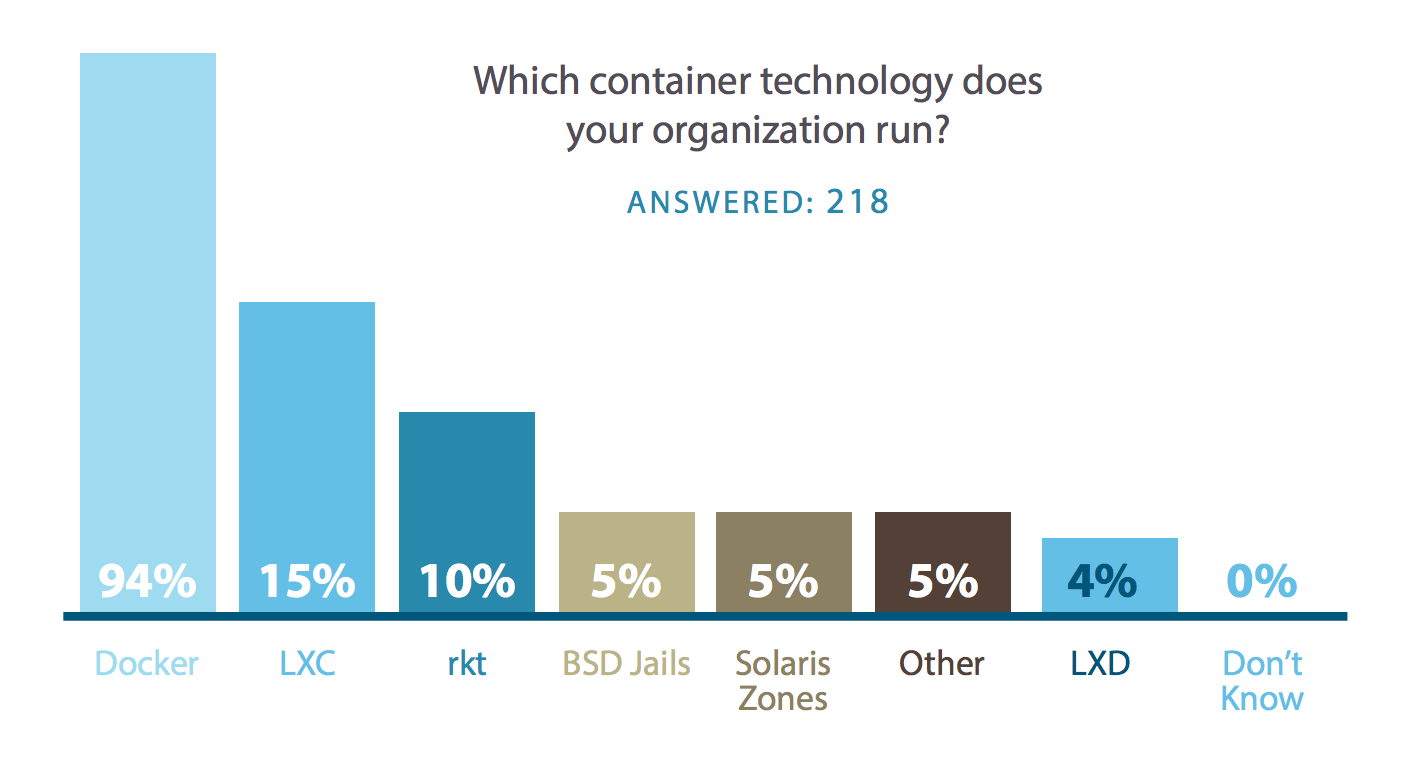
\includegraphics[width=0.8\textwidth]{images/docker.png}
    \par
	  \caption{Nejpoužívaněší kontejnerové technologie\label{fig:container}, zdroj: \source{\cite{picture}}}
    \end{centering}
\end{figure}

\subsubsection{Docker}
Součástí Dockeru je několik technologií. Mezi ně patří specifikace kontejnerů, runtime neboli běhové prostředí kontejnerů jehož součástí jsou Dockerfiles, které umožnují opakovatelné vytváření kontejnerů. Součástí je i technologie Docker Hub, která slouží jako uložiště kontejnerů. Docker projekt byl vytvořen v roce 2013 v programovacím jazyce Golang. Následující kapitola je vypracována s využitím zdroje \cite{docker-security}.\par
Docker image je označení pro obraz dané aplikace se všemi spustitelnými soubory, závislostmi, knihovnami a také konfiguračními soubory. Docker image se skládají \linebreak z vrstev společně s metadaty. Každá vrstva obsahuje informace o změně, která byla provedena vůči předchozí vrstvě. Na obrázku \ref{fig:container-layers} je znázorněn systém přidávání jednotlivých vrstev. Vše začíná base, základním, imagem ze kterého potom vychází další vrstvy. Na base image navazuje přidání Apache serveru, poté přidání verzovacího systému Git a nakonec přidání souborů pro spuštění aplikace. Každá vrstva má svého předka a tím je předchozí vrstva. Vyjímkou je první vrstva, base image, která žádného předka nemá. Base image může být například klasická linuxová distribuce jako jsou Debian nebo CentOS a také minimalistický Alpine linux. Použití vrstev dovoluje doručovat image jako soubor modifikací nad určitým imagem. \par

\begin{figure}[H]
  \begin{centering}
    
    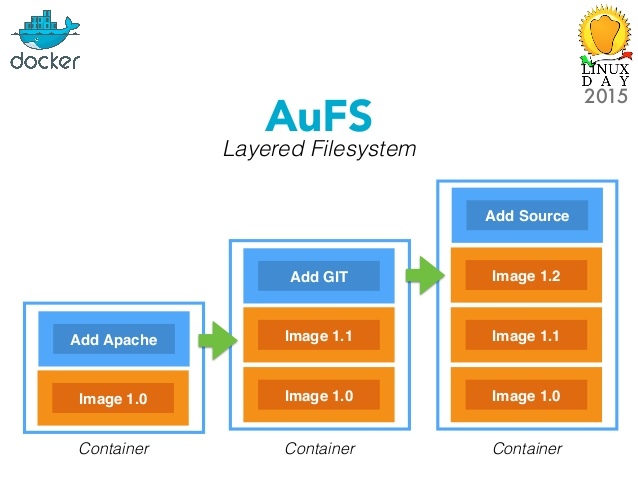
\includegraphics[width=0.8\textwidth]{images/container-layers.jpg}
    \par
	  \caption{Kontejnerové vrstvy\label{fig:container-layers}, zdroj: \source{\cite{picture-docker-layers}}}
    \end{centering}
\end{figure}

Existují dva způsoby, jak je možné vytvořit docker image. Prvním z nich je spustit existující image a v něm provést změny. Například nainstalovat nový balíček, poté kontejner zastavit a vytvořit z něho nový kontejner s provedenými změnami. Tento proces není flexibilní a je nutné všechny kroky provézt znovu při vytváření image. \linebreak K automatizaci vytváření docker image slouží nástroj Dockerfiles. Tento nástroj vytvoří podle definice kontejnery se všemi potřebnými závislostmi a soubory. Formát a syntaxe DockerFile souboru na ukázce kódu \ref{lst:dockerfile} specifikuje base image ze kterého kontejner vychází. Dále odkud a jaký balíček má být nainstalovaný nebo také jaký příkaz se má vykonat při startu kontejneru. \par

\begin{centering}
	\begin{lstlisting}[caption={Příklad docker file souboru},label=lst:dockerfile]
FROM golang:1.12
ENV version=1.11
WORKDIR /go/src/app
COPY basicHttp .
RUN chown golang:golang basicHttp
ENTRYPOINT ["./basicHttp"]
EXPOSE 80
\end{lstlisting}
\end{centering}

Docker běží jako daemon na serveru a spravuje kontejnery. Tento program spouští kontejnery, kontroluje úroveň izolace jednotlivých kontejnerů, ověřuje, že kontejnery využívají pouze přidělené zdroje. Jednou z činností, které daemon vykonává je sledování stavu kontejnerů a vykonání adekvátních akcí, např. restart kontejnerů. Daemon je také zodpovědný za správu images, konkrétně stáhnutí z , případně nahrání image do vzdáleného docker registry. Docker daemon také zodpovídá za vytváření images přes Dockerfiles. Docker registry je repozitář, kam uživatelé mohou nahrávat své kontejnery a také odtud kontejnery stahovat. Příkladem Docker registry je DockerHub. Vývojáři se mohou zaregistrovat a využívat repozitář pro sdílení images. \par
Pro oddělení jednotlivých zdrojů kontejnerů používá Docker Namespaces, neboli jmenné prostory. Namespaces izolují procesy, síťová zařízení, mount pointy a uživatele uvnitř kontejneru před ostatními procesy zdroji na serveru. Jedním typem je PID namespace. Tento namespace izoluje skupinu procesů. Tyto procesy jsou izolované a nevidí ostatní procesy mimo namespace. Z pohledu kontejneru jsou všechny procesy potomkem procesu s PID 1 a čísla procesů se mohou v jednotlivých namespace opakovat \cite{namespaces}. Druhou významnou technologií, kterou Docker použivá jsou Cgroups. Cgroups je mechanismus jak omezit využití zdroje pro proces nebo skupinu procesů. Není tak možné aby jeden kontejner zabral všechny zdroje serveru pro sebe a blokoval tak ostatní kontejnery. Cgroups tak dovolují přiřadit kontejneru pouze omezené zdroje jako jsou čas na procesoru, RAM, využití sítě či disku \cite{cgroup}. Obě technologie jsou součástí linuxového jádra od verze 2.6.24.\par
\subsubsection{Rkt}
Rkt projekt byl vytvořený společností CoreOS a jeho hlavním účelem bylo odstranit nedostatky dockeru. Rkt je open source bezpečnější alternativa k Dockeru. Rkt také umožňuje spustit více izolovaných images, které sdílejí jádro systému. Rkt poskytuje větší bezpečnost než docker images. Například při stahování image z registry, docker nekontroluje image. Na druhé straně Rkt ověřuje podpis vydavatele dané image \cite{ROCKET}. Rkt také podporuje řízení přístupu SELinux, případně umožňuje spustit kontejner s aplikací ve virtuálním serveru \cite{selinux}. Rkt používá ACI (Application container format) image format a jako základní jednotku nasazení využívá Pod. Pod je seskupení jednoho nebo více images aplikace (ACI images). Jednotlivé images uvnitř podu sdílejí přidělené zdroje, například networking. Rkt je schopný spouštět jak ACI formát images tak i Docker formát. Rkt také implementuje OCI standard, který je představen v další kapitole.
\subsubsection{Open container initiative}
Open container initiative (OCI) je projekt, který má za cíl vytvořit standardy týkající se formátu kontejnerů a také běhového prostředí kontejnerů. Tento projekt byl vytvořen v roce 2015 lídry v oboru kontejnerových technologií Docker a Rkt. OCI aktuálně zahrnuje dvě specifikace \cite{oci}. \par
První je runtime specifikace, která specifikuje konfiguraci, spouštěcí prostředí a životní cyklus kontejneru. Konfigurace se specifikuje ve formátu JSON a obsahuje informace o verzi OCI specifikace, procesy, které mají být spuštěné, uživatelé, proměnné prostředí a další metadata. Standardizované spouštěcí prostředí zajištuje, že aplikace běžící uvnitř kontejneru poběží stejně v různých runtime prostředích. Poslední částí je specifikace příkazů, které je možné na daném kontejneru provézt \cite{runtimespec}.\par
Druhou specifikací je formát images. Tento formát definuje, že image splňující OCI specifikaci se skládají z manifestu, sadu vrstev souborového systému, konfiguraci a \linebreak nepovinný image index. Manifest soubor obsahuje informace o image jako jsou konfigurace a sada vrstev pro jeden kontejner. Ve specifikaci je popsáno jak vytvářet a používat jednotlivé vrstvy souborového systému kontejneru. Konfigurace je popis změn provedených na jednotlivých vrstvách \cite{imagespec}. 

\subsection{Orchesrátory}
Microservices architektura rozděluje aplikaci na menší části, které se lépe spravují. Technologie kontejnerů zabaluje jednotlivé microservices do samostatných kontejnerů společně s jejich závislostmi. Kontejnery dovolují spustit aplikaci se stejným výsledkem v různých prostředích bez nutnosti konfigurace aplikace. Pokud spravujeme dvě aplikace v deseti kontejnerech je možné veškerou správu aplikace a kontejnerů provádět ručně. Pokud ovšem provozujeme stovky aplikací v tisíci a více kontejnerech, manuální správa kontejnerů se stává velice obtížnou. Zde přicházejí na řadu orchestrátory kontejnerů. Orchestrátory provádějí následující úkony \cite{container-orchestration}:
\begin{itemize}
\item Orchestrátor se stará o stažení požadovaného image a jeho následné spuštění na vhodném serveru. Tento proces začíná předáním konfigurace orchestrátoru. Orchestrátor z konfigurace získá potřebné informace. Například odkud má stáhnout požadovaný image, na jakých portech by měla daná aplikace poslouchat, dále také jaké uložiště má být ke kontejneru připojeno, připojení kontejneru do sítě, aby mohl komunikovat a byl dostupný, vložení konfiguračních souborů pro aplikaci a přiřazení dalších metadat danému kontejneru. Orchestrátor také musí rozhodnout na jakém serveru kontejner spustit. Snahou je rovnoměrně zatěžovat jednotlivé servery, které hostí kontejnery a také přiřadit kontejnerům potřebné zdroje. Orchestrátor je i zodpovědný za správné ukončení aplikace. Například databáze bude vypnuta šetrně, aby nedošlo k poškození dat. Všechna potřebná data budou zapsána, transakce potvrzeny a poté dojde k uvolnění využívaných zdrojů.
\item Dalším úkolem orchestátoru je sledování běžících kontejnerů a jejich správa. Orchestrátor sleduje stav jednotlivých kontejnerů, jestli fungují jak mají. Pokud se například aplikace uvnitř kontejneru zastaví, kvůli chybě, orchestrátor to musí zjistit a namísto starého kontejneru vytvořit nový. Orchestrátor sleduje jednotlivé zdroje a udržuje takový stav jaký je definovaný v konfiguraci pro danou aplikaci. Jedním z aspektů, které orchestrátor kontroluje je i kolik zdrojů kontejner využívá a zda nepřekračuje přiřazené limity využívání. 
Orchestrátor nedohlíží pouze na stav kontejnerů, ale sleduje také stav serverů, které hostují kontejnerizovanou aplikaci. Pokud dojde k poruše serveru nebo jeho vypnutí, orchestrátor tuto akci zaznamená a všechny kontejnery, které na nedostupném serveru běžely jsou spuštěny na jiných běžících serverech. Na nedostupný server také nejsou posílány požadavky na spuštění kontejnerů, dokud není server obnoven.
\item Jednou z výhod cloud native přístupu je škálovatelnost aplikací, kterou orchestrátory kontejnerů také zvládají. Orchestrátor umí na požádání přidat další instance aplikace. Například ve špičce při velkém zatížení jsou orchestrátory schopné automaticky navýšit počet kontejnerů dané komponenty. Orchestrátory též zajišťují load-balancing, neboli rozložení požadavků mezi všechny spuštěné instance aplikace. Příkladem může být webový server. V konfiguraci aplikace jsou specifikovány tři instance tohoto serveru. Uživatelské požadavky jsou rovnoměrně, případně podle jiného algoritmu, přesměrovány na jednotlivé instance webového serveru. Pokud se jeden z webových serverů porouchá, orchestrátor tuto informaci zjistí pomocí pravidelných kontrol a nepřesměrovává uživatele na tento kontejner. 

\item Pro přístup uživatelů k aplikacím z vnějšího světa, umožňují orchestrátory vystavit službu pomocí portu na veřejné adrese. Uživatelé se tak mohou jednoduše připojit na danou aplikaci a využívat služby, které nabízí. 
\item Další oblastí, kterou orchestrátory pokrývají je monitoring aplikací. Orchestrátory nabízejí různé statistiky o využití jednotlivých kontejnerů. Dále umožňují procházet logy jednotlivých služeb pro řešení problémů. 
\end{itemize}
\par
Orchestrátory kontejnerů dávají správcům aplikací mnoho výhod. Jednou z nich je jednotný přístup ke správě aplikací. Pro správu kontejnerizovaných aplikací používají správci stejné nástroje. Dalším aspektem je automatizace nasazení aplikace, přechod na novější verzi, škálování a dostupnost aplikace. Správci mohou automatizovat i jednotlivé kroky údžby aplikace. Tento přístup umožňuje cílit hlavně na vylepšování aplikace samotné v porovnání s manuálním přístupem ke správě kontejnerizované aplikace. Při manuální správě jsou zaměstnanci většinu času zabráni do udržování dostupnosti aplikace, nasazování nových verzí atd. Manuální řešení není vhodné pro větší a dynamické projekty, protože zvětšování počtu lidí, kteří tuto práci provádějí není udržitelné. Orchestrátory zjednodušují a zrychlují správu větších a rostoucích projektů v dynamickém prostředí, které vyžaduje periodické přidávání a ubírání jednotlivých kontejnerů. Ke správě velkého počtu kontejnerů tak není zapotřebí armáda inženýrů, ale postačí malý tým operátorů pracujících s orchestrátorem. \par
    Pokud si připomeneme Pets vs Cattle concept správy serverů z předchozí kapitoly, orchestrátory nakládají s kontejnery jako s Cattle, tedy dobytkem. Orchestrátor se nestará o jednotlivé kontejnery jako o Pets, neboli mazlíčky. Pokud je kontejner v chybovém stavu, nebo je nedostupný, dojde k jeho vypnutí a nahrazení jiným kontejnerem, který převezme jeho funkci. Společnost Sysdig ve své zprávě o využívání kontejnerů \cite{sysdig} uvádí, že ze zjištěných dat je životnost 95\% kontejnerů maximálně týden. Z dat dále vyplývá, že nejvíce procent kontejnerů, konkrétně 27\%,  má životnost mezi pěti až deseti minutami. Tato data ukazují, že správa kontejnerů je velice dynamická. Orchestrátory dále dávají jasný pohled na běžící aplikaci a minimalizují tak manuální zásahy do systému o kterých ví pouze daný operátor. Manuální změny uvnitř kontejnerů nejsou perzistentní, při ztrátě kontejneru dojde i ke ztrátě manuální změny. Tento fakt napomáhá přenositelnosti aplikace mezi jednotlivými prostředími a zaručuje, že co funguje v testovacím prostředí bude fungovat v produkci. V dalších kapitolách budou představeny konkrétní orchestrátory kontejnerů. Sysdig zpráva o využívání kontejnerů \cite{sysdig} také uvádí hlavní tři nástroje na správu kontejnerů. Nejpoužívanějším nástrojem je Kubernetes, následované nástrojem Docker Swarm třetím nástrojem je Mesos Marathon. Tyto nástroje jsou představeny dále v kapitole.

 \subsubsection{Docker Swarm}
 Docker Swarm, jak už název napovídá, byl vytvořen společností Docker v roce 2015. Docker Swarm používá stejné standardní Docker API. To znamená, že všechny nástroje, které jsou schopné komunikovat s Dockerem (např. Docker CLI, Docker Compose) mohou stejně komunikovat i s Docker Swarmem. Výhodou je, že uživatelé mohou používat stejné nástroje, které už znají. Na druhé straně funkcionalita je omezena pouze na Docker API. \par
     Swarm spojuje jednotlivé servery, které jsou schopny spouštět Docker kontejnery do jednoho virtuálního serveru. Uživatel má dojem, že přistupuje pouze k jedné instanci Docker serveru, ve skutečnosti je na pozadí několik takovýchto serverů. Docker přidává další 2 nástroje Docker machine a Docker Compose. Docker machine slouži pro instalaci Docker engine na fyzické nebo virtuální servery, které budou hostovat Docker kontejnery. Pomocí Docker Compose je možné definovat pomocí YAML syntaxe chování kontejnerů a ty poté spustit. Příklad compose file na ukázce kódu \ref{lst:compose}.\par
         Docker Swarm vyniká především svou jednoduchostí instalace i použití. Docker Swarm je součástí Docker engine a používá stejné nástroje jako Docker. Swarm \linebreak umožňuje spravovat skupinu serverů, které jsou schopné běžet kontejnery, jako jeden virtuální server.

\begin{lstlisting}[caption={Příklad docker compose souboru},label=lst:compose]
version: '2'
services:
  nsqlookupd:
    image: nsqio/nsq
    command: /nsqlookupd
    ports:
    - "4160:4160"
    - "4161:4161"
  nsqd:
    image: nsqio/nsq
    command: /nsqd --lookupd-tcp-address=nsqlookupd:4160
    depends_on:
    - nsqlookupd
    ports:
    - "4150:4150"
    - "4151:4151"
  nsqadmin:
    image: nsqio/nsq
    command: /nsqadmin --lookupd-http-address=nsqlookupd:4161
    depends_on:
    - nsqlookupd  
    ports:
    - "4171:4171"
\end{lstlisting}

\subsubsection{Mesos Marathon}
Mesos poskytuje vrstvu abstrakce nad fyzickými servery v datovém centru nebo nad velkými výpočetními zdroji. Mesos kombinuje zdroje jako jsou CPU, RAM a datové uložiště do jednoho sdíleného prostoru, aby zdroje byly využívány co nejefektivněji. Tento prostor je abstrakce nad jednotlivými servery a jeví se jako jeden velký server. Odtud jsou zdroje přiřazovány jednotlivým běžícím aplikacím podle jejich požadavků. Aplikace běžící na Mesosu vidí tuto abstrahovanou vrstvu jako vysoce dostupný,  odolný proti chybám a distribuovaný operační systém. Mesos je systém, který je \linebreak schopný nabídnout škálovatelnost a odolnost vůči výpadkům velkým a náročným aplikacím. Apache mesos využívají například Apple pro svou hlasovou službu Siri, dále například společnost Bloomberg nebo PayPal. Funkce Mesosu mohou být rozšířeny pomocí modulů \cite{delvalle}. \par
    Architekturu řešení Mesos můžeme vidět na obrázku \cite{mesos-picture}. Mesos se skládá z Masteru, který řídí agenty, dříve nazývané jako slaves. Agenti běží na fyzické serveru v datacentru. Jednotlivé moduly spouštějí s využitím master serveru úlohy na agentech. Moduly komunikují s masterem přes RestApi volání. Master servery pracují v active-passive módu. Pouze jeden master je aktivní. Pro výběr aktivního serveru používá Mesos nástroj Zookeeper. Obě komponenty Mesos master a Zookeeper běží v režimu vysoké dostupnosti, kdy při výpadku jednoho ze serverů je Mesos schopen fungovat dále. \par
	Agenti oznamují primárnímu masteru zdroje, které mají k dispozici. Master poté nabízí tyto zdroje jednotlivým modulům. Modul si vybere z nabízených zdrojů, tak aby splňovaly požadavky na úlohu, kterou chce spustit. Modul poté oznámí aktivnímu master serveru na jakém agentovi vybranou úlohu spustit. Například orchestrátor kontejnerů pro systém Mesos se nazývá Marathon.\par
	Marathon podporuje běhové prostředí kontejnerů Mesos containers a také Docker. Modul dále dovoluje připojení persistent storage pro stavové aplikace jako jsou \linebreak databáze. Součástí je webové rozhraní pro práci s kontejnery, RestApi pro automatizaci a integraci s dalšími projeky, dále sada pravidel pro kontejnery. Marathon obsahuje nástroje pro service discovery, neboli katalog dostupných služeb, load-balancing, kontrolu dostupnosti služeb, metriky a statistiky \ref{fig:mesos}.


\begin{figure}[H]
  \begin{centering}
	  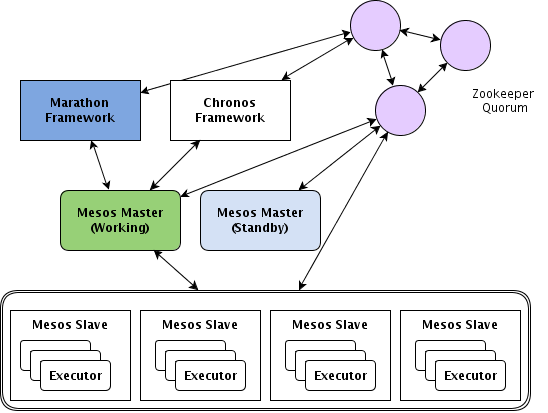
\includegraphics[width=0.8\textwidth]{images/mesos.png}
    \par
	  \caption{architektura Mesos orchestrátoru\label{fig:mesos}, zdroj:\source{\cite{mesos-picture}}}
    \end{centering}
\end{figure}

\subsubsection{Kubernetes}
Kubernetes je open source orchestrátor kontejnerů. Kubernetes, zkráceně k8s, nabízí širokou škálu funkcí. K8s bylo vytvořeno společností Google, ale poté bylo připojeno k CNCF. K8s se stalo de facto standardem pro orchestraci kontejnerů a to díky velké komunitě okolo tohoto projektu. O úspěchu projektu svědčí také podpora k8s napříč cloud providery jako jsou Google Cloud Engine, Microsoft Azure a AWS. \par
K8s je platforma pro orchestraci nasazení, škálování a správy aplikací běžících v kontejnerech. Kapitola o Kubernetes je vypracována s využítím zdroje \cite{MASTERING-KUBERNETES}. Mezi funkce k8s patří možnost připojení souborového systému do kontejneru, distribuce citlivých informací, jako jsou hesla nebo tokeny, v podobě hashe mezi kontejnery pomocí tkz. Secrets. K8s umí také udržovat stanovený počet replik jednotlivých kontejnerů, škálovat aplikace, monitorovat zdroje, zpřístupnit logy jednotlivých kontejnerů a mnoho dalšího. \par
Architektura k8s je zobrazena na obrázku \ref{fig:k8s}. K8s se skládá ze dvou základních částí, první je master role a druhá je node role a ty jsou dále tvořeny dalšími komponentami. Jednotlivé role mohou být nasazeny jak na fyzických tak i virtuálních serverch. \par

\begin{figure}[H]
  \begin{centering}
	  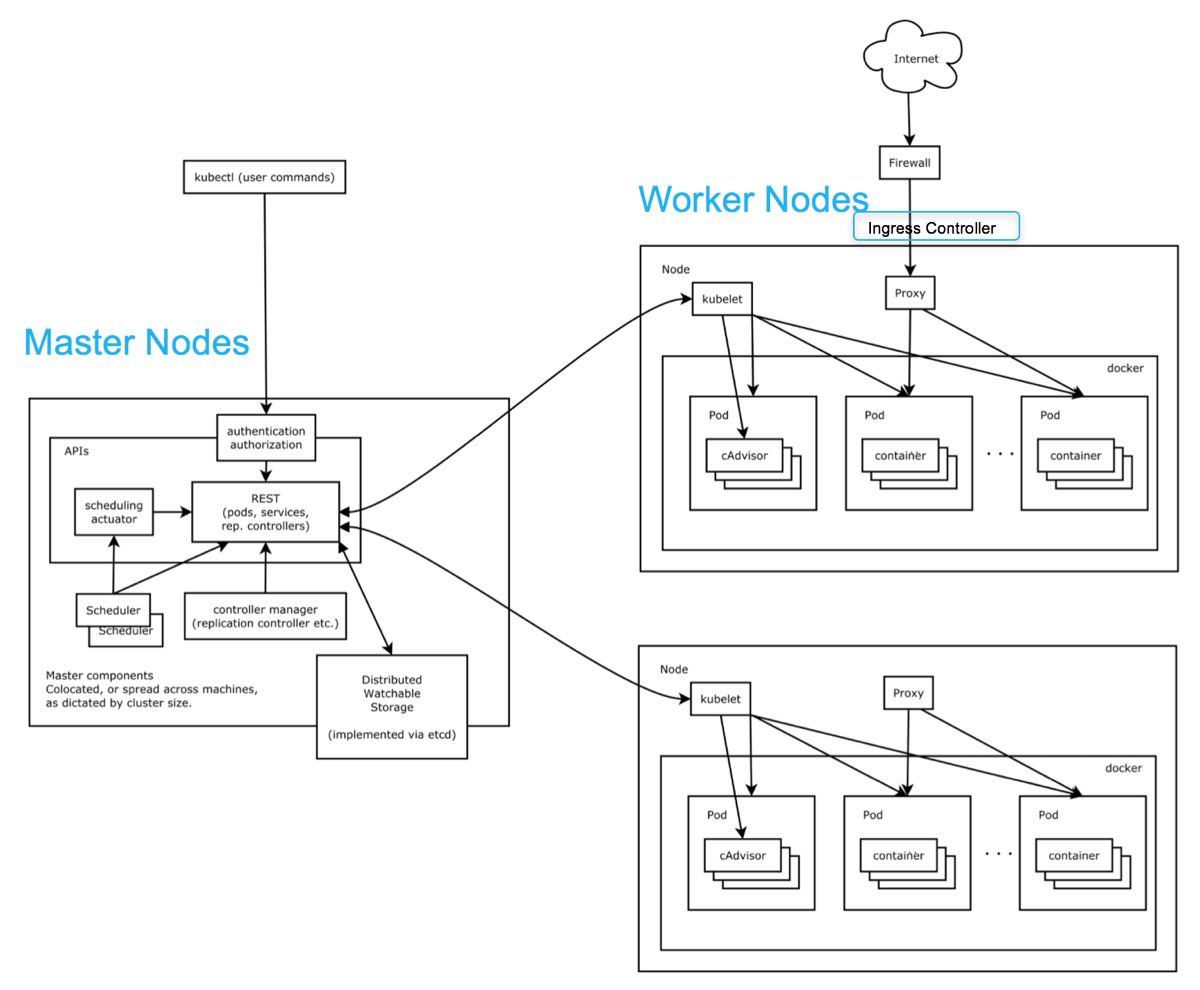
\includegraphics[width=0.99\textwidth]{images/k8s-architecture.png}
    \par
	  \caption{architektura Mesos orchestrátoru\label{fig:k8s}, zdroj: \soucre{\cite{k8s-architecture}}}
    \end{centering}
\end{figure}

Master server tvoří control plane Kubernetes a je zodpovědný za nasazování a správu podů a také obsluhu různých událostí. Master server tvoří komponenty API server, scheduler a controller. API server vystavuje REST API, přes které může probíhat komunikace s Kubernetes. Ke kubernetes API můžeme přistupovat pomocí nástroje Kubernetes CLI přímo z příkazové řádky, s využitím klientské knihovny a také přímo dotazy na API. Jednotlivé akce nabízené k8s tak mohou být automatizovány. Api server jednoduše škáluje, protože data o běžících kontejnerech a stavu celého clusteru si \linebreak uchovává v Etcd databázi. Controller je komponenta, která sleduje stav clusteru přes API server a řídí celý cluster k tomu aby byl v požadovaném stavu. Do controlleru patří pod controller, replica controller a také service controller. Například replica controller sleduje počet běžících podů a snaží se udržet definovaný počet instancí daného podu. Pokud existuje více podů, replica controller vypne přebývající pody a pokud je naopak podů méně, replica controller nastartuje další pod. Scheduler je komponenta, která je zodpovědná za spuštění podů na nodech. Scheduler musí rozhodnout, který node má dostatečnou kapacitu pro běh daného kontejneru nebo pokud node splňuje určité požadavky jako například SSD disk nebo možnost připojení grafické karty a další.     \par          
Druhou komponentou je Node server, jehož úkolem je běh jednotlivých podů. Node server je řízený k8s master komponentou. Node interaguje s masterem z něhož získává informace jaký workload má spustit a zpět zasílá informace o workloadu do masteru. Kubernetes node je dále složen z kubeletu a kube proxy. Kube proxy je služba běžící na každém nodu, která může vykonávat jednoduché TCP/UDP směrování. Například vytváří virtuální adresy pro services, tak aby pody byly schopné komunikovat s ostatními pody v clusteru. Kubelet komunikuje s master komponentou, řídí a spravuje běžící pody. Mezi činnosti Kubeletu patří stahování secrets z API serveru, připojování uložiště do kontejnerů, provozování kontejnerů, oznamování API serveru svůj stav, stav nodu, a také stav běžících podů. Kubelet řídí kontejnery uvnitř podu pomocí CRI (Container runtime interface). CRI je soubor specifikací, požadavků a knihoven, které musí kontejnerové běhové prostředí (runtime) splňovat, aby mohlo být použito jako runtime kontejnerů pro k8s. K8s podporuje několik runtime prostředí, konkrétně Docker, Rkt, Cri-o nebo Containerd. Součástí k8s jsou i další koncepty a zdroje jako jsou pods, services, secrets, labels, replication controllers, volumes a další.   \par
Základním stavebním kamenem k8s je pod. Pod obsahuje jeden nebo více kontejnerů. Kontejnery uvnitř jednoho podu jsou spuštěny najednou na stejném nodu. \linebreak Všechny kontejnery v podu sdílejí jeden síťový prostor. To znamená, že mají stejnou ip adresu, sdílejí síťové porty a mohou komunikovat přes localhost adresu. Různé kontejnery v podu tedy musí používat rozdílné porty. Všechny kontejnery v podu mohou přistupovat ke sdílenému lokálnímu uložišti. Pody nejsou považovány za perzistentní, jsou vytvářeny a mazány na požádání. Při smazání podu jsou smazána i všechna data. K tomu aby se data uchovala se používá koncept volume.\par
Aby bylo možné vybírat specifické pody, například pody s určitou verzí aplikace, představuje k8s label, neboli popisek. Labels jsou popisky tvořené jako klíč a hodnota každý pod může mít více labels. Label používá ostatní zdroje pro identifikaci podů.\par
Dalším zdrojem je Replication Set, který spravuje skupinu podů, které jsou vybírány na základě label. Replication set zajišťuje, že definovaný počet podů je spuštěn. Pokud dojde k havárii jednoho nebo více z podů, Replication set vytvoří nový pod, aby byl jejich počet rovný definovanému stavu. Pokud je vytvořen pod s labelem, který se shoduje s definicí v replication setu, čímž dojde k překročení počtu instancí daného podu, je tento pod zastaven. \par
Pro load-balancing a redundancy podů poskytuje k8s services koncept. Services mají za úkol zpřístupnit uživatelům nebo dalším službám určitou funkcionalitu. Services používají label k výběru skupiny podů. Service poté rozděluje požadavky mezi jednotlivé pody v dané skupině. Pomocí service můžeme například vystavit aplikaci na určité adrese a portu pro externí uživatele. Další použití může být pro komunikaci jednotlivých microservices. Pody nekomunikují přímo s ostatními pody, ale přistupují na service, která load-balancuje mezi pody, jejichž label se shoduje s definicí v service.\par
Jak již bylo zmíněno data v podech nejsou persistentní, pokud je pod zničen všechna data jsou ztracena. Pokud potřebujeme, aby data zůstala i po zničení podu můžeme využít volume. Data je tak možné sdílet mezi kontejnery v podu a také přežijí restart podu. Pro stateful aplikace jako jsou například databáze nabízí k8s koncept stateful setu. Stateful set asociuje volume s daným specifickým podem. Pody řízené stateful setem mají stanovený neměnný hostname. Záleží na pořadí v jakém jsou spuštěny. Pokud definujeme 3 instance nejdříve bude spuštěn první s označení například mysql-0 a další v pořadí mysql-1 bude spuštěn až když mysql-0 je připraven a funkční. Na druhé straně při vypnutí je nejdříve vypnutý pod mysql-2, tedy poslední, po dokončení vypnutí se začne vypínat mysql-1 a tak dále. Stejně jako mají pody statefulsetu neměnný hostname, nemění asi ani volum, který mají připojený. To znamená, že mysql-1 bude mít vždy připojený stejný volume.\par
Pro oddělení jednotlivých podů se v k8s používá namespace. Namespace je virtuální cluster uvnitř fyzického clusteru. Jednotlivé zdroje uvnitř jednoho namespace jsou izolované od ostatních zdrojů v jiném namespace a komunikovat spolu mohou pouze přes veřejné rozhraní. \par
Kubernetes nabízí širokou škálu funkcí a možností jak spravovat aplikace v kontejnerech. K8s architektura je modulární a je možné vyměnit jakoukoliv část vlastním řešením a rozšířit tak funkcionalitu k8s. Například scheduler služba na master serveru může být nahrazena libovolnou službou, která bude implementovat jiný algoritmus pro vybírání nodů, na kterých bude workload spuštěn. Další velkou oblastí je networking. Pro k8s existuje mnoho nástrojů, které se starají o komunikaci mezi jednotlivými pody, services a také příchozí komunikaci z vnějšku. Mezi zástupce patří Project Calico \cite{calico}, Flanel \cite{flanel}, nebo Weave Net \cite{weave}. 


\chapter{Hybrid cloud}
Hybrid cloud je typ cloudového prostředí, které kombinuje privátní a veřejný typ cloudu čímž dovoluje využít výhod obou řešení pro běh aplikací a sdílení dat. Každá část hybrid cloudu zůstává samostatná a unikátní, ale je pomocí standardizované nebo proprietární technologie napojená na ostatní nasazené modely. Toto spojení umožňuje jednotlivým aplikacím vzájemnou komunikaci. Hybrid cloud je tvořen spojením nejméně jednoho private cloudu a jednoho public cloudu [goyal2014public]. \par
    Hybrid cloud řešení snižuje CAPEX (Capital expenditure) náklady, protože část firemní infrastruktury je spravována poskytovatelem public cloud řešení. CAPEX náklady znamenají výdaje na pořízení výměnu a správu hardwaru a také pořízení vybavení datacentra. Hybridní řešení dále vylepšuje přiřazení zdrojů pro dočasné projekty. Využití public cloud řešení odstraňuje investice, které jsou potřeba během projektů. Odpadá tedy nutnost zakoupit hardware pro každý nový projekt. Tyto zdroje jsou alokovány na straně public cloudu. Po dokončení či zrušení projektu je snadné tyto zdroje opustit a společnost za ně nemusí nadále platit. Přidání zdrojů a odebrání zdrojů je snadné a napomáhá společnosti pokrýt sezónní nápor uživatelů. Tento přístup nabízí uživateli snadnou škálovatelnost a pomáhá optimalizovat náklady. \par
        Cílem hybrid cloudu je kombinovat výhody public a private cloudu. Z modelu private cloudu si hybrid cloud bere především bezpečnost dat. Společnost tak může mít nasazenou aplikaci v prostředí public cloudu a data se kterými aplikace pracuje jsou uložena v privátním datacentru. Public cloud poskytne škálovatelné prostředí a privátní cloud zase zabezpečí, že data jsou uložena na serverech vlastněných a spravovaných společností v požadované zeměpisné lokaci. Společnost má s hybrid cloud modelem kritická data pod kontrolou. \par
	Další oblastí využití modelu hybridního cloudu je oblast edge computingu. Edge computing je vhodný pro oblasti, které potřebují spolehlivou a rychlou síťovou konektivitu. Model hybridního edge cloudu se na tyto problémy zaměřuje a snaží se je řešit. Pro byznys důležité aplikace je užitečné provozovat lokálně v místě vzniku dat s kterými pracují. Díky tomu jsou splněny požadavky na rychlou odezvu. Pro hybrid edge model není internetové spojení mezi edge cloudem a centrálním cloudem kritické. Používá se především pro správu edge prostředí a výměnu dat. Aplikace využívají lokální výpočetní zdroje. Synchronizace dat mezi edge a centrálním cloudem probíhají na pozadí, používají zabezpečené spojení. Při výpadku spojení mezi edge a centrálním cloudem zůstávají všechny aplikace funkční a data se ukládají lokálně, dokud není spojení obnoveno. Poté jsou přesunuty do centrálního cloudu k dalšímu zpracování. Edge tak není závislý na centrálním cloudu.\par
	Architektura hybrid edge modelu je zobrazena na obrázku [edge-picture]. Kritické a důležité aplikace běží v edge cloudu. V centrálním cloudu, v tomto případě GCP (Google Cloud Platform), běží centrální control plane pro jednotlivé edge cloudy a také monitoring, který agreguje data a poskytuje centrální správu a globální pohled na celé řešení. S využitím kontejnerů a například Kubernetes, které je podporované většinou poskytovatelé veřejného cloudu, odstranit rozdíly mezi jednotlivými edge lokacemi a centrálním cloudem. K8s zaručí stejné běhové prostředí pro kontejnery a podle potřeby dovoluje například přesouvat workload mezi edge cloudem a centrálním cloudem [google-edge]. V následující kapitole jsou představeny jednotlivé nástroje, které je možné použít pro správu hybrid prostředí.

\subsection{Existující řešení pro hybrid cloud}

\subsubsection{Red Hat Cloudforms/Manage IQ}
Cloudforms je platforma pro jednotnou správu fyzických a virtuálních serverů a také kontejnerů napříč různými cloudovými prostředími. Pomocí CloudForms je možné ovládat zdroje v technologiích pro privátní cloudy OpenStack a také virtuální servery spravované technologií od společnosti VMware, Red Hat virtualization a Microsoft Hyper-V. CloudForms umožňuje spravovat zdroje ve veřejných cloudech AWS (Amazon web services), Microsoft Azure a také GCP (Google cloud platform). CloudForms umožňuje spravovat také kontejnery na platformě OpenShift. CloudForms technologie vychází z Manage IQ technologie. Manage IQ je jednotná open-source platforma pro správu cloudových prostředí. Cloudform je vyvíjeno, spravováno a podporováno přímo společností Red Hat, jedná se o komerční řešení. Manage IQ je stejná platforma s otevřeným kódem, která je spravována a rozvíjena komunitou napříč různými společnostmi [manageiq]. Dále v textu je popisována Manage IQ verze.\par
    Manage IQ přistupuje k jednotlivým systémům, označovaným jako poskytovatelé, přes API, které např. veřejné cloudy nebo OpenStack poskytují. Přes tato API si Manage IQ vyčítá informace o jednotlivých zdrojích  jako jsou virtuální servery, kontejnery, load-balancery společně s jejich metadaty jako jsou jméno, typ a mnoho dalšího. Tyto zdroje jsou označovány jako managed elements, neboli spravovaný prvek, a jsou uloženy ve Virtual Managemet Database (VMDB). Manage IQ po počátečním získání informací z jednotlivých poskytovatelů stále sleduje jednotlivá API poskytovatelů a udržuje VMDB stále aktuální. Manage IQ poskytuje přehledné webové rozhraní ve kterém jsou zobrazeny jednotlivé zdroje poskytovatelů s detailními informacemi. Například při připojení na VMware je zobrazen seznam běžících virtuálních serverů společně s jejich atributy jako je počet jader, velikost RAM, operační systém, připojení sítě, nainstalované programy a tak dále. \par
    Manage IQ dovoluje provádět akce nad objekty, které má zaregistrované ve VMDB. Například virtuální servery běžící ve VMware prostředí můžeme vytvářet, mazat, vypínat, zapínat a restartovat. Další oblastí správy zdrojů je sledování a provádění změn. Můžeme sledovat jednotlivé atributy zdrojů a také kdy došlo k jejich změně. Manage IQ umožnuje také porovnávat aktuální stav s počátečním stavem. Např. jaké změny byly provedeny na virtuálním serveru oproti jeho základní konfiguraci. Manage IQ může zaznamenat změnu sudo práv, přidání nového uživatele nebo nainstalování nového balíčku. Protože Manage IQ má data o všech zdrojích jednotlivých poskytovatelů, můžeme s jeho pomocí počítat náklady na provoz.\par
    Další věcí, kterou Manage IQ nabízí jsou služby. Služby dovolují vytváření složitějších konfigurací jednoduchou cestou. Přes služby můžeme například vytvořit dva virtuální servery s nainstalovaným webovým serverem, jeden server poběží v prostředí OpenStacku a druhý na VMwaru. Dále virtuální server sloužící jako databáze a poté ještě load-balancer, který bude rozkládat zátěž mezi webové servery. Výběr těchto zdrojů může například sloužit vývojářům aplikace jako prostředí pro vývoj. Vytvořit takovéto prostředí bude možné na jedno kliknutí. Správce vytvoří podle požadavků skript, který tyto zdroje vytvoří a poté zdroje nastaví. Vývojáři mohou z webového rozhraní skript spustit a během chvíle dostanou připravené prostředí pro vývoj. Tento nástroj dovoluje vytvářet složitější konfigurace a jednoduše je nasadit. Vývojáři tak tráví více času programováním aplikace namísto nastavování serverů. Administrátoři mohou povolit přistup k určitým zdrojům pouze uživatelům, kteří splnují stanovená pravidla. Např. pouze uživatelé ve skupině vývojáři mohou spouštět skript, který vytvoří vývojářské prostředí z předchozího příkladu [lwn].

\subsubsection{Cloud foundry}
Cloud Foundry (CF) je open source cloudová PaaS platforma. Na této platformě mohou vývojáři jednoduše vytvořit, nasadit, běžet a škálovat aplikace. CF bylo původně vytvořeno společností VMware. Později došlo ke zveřejnění zdrojových kódů a stalo se komunitním projektem. Jedná se o Paas řešení, které je dobře nastavitelné a rozšiřitelné, uživatelé mohou používat širokou škálu frameworků a programovacích jazyků. CF může být nasazeno na vlastní hardware případně na jinou podporovanou cloud platformu jako je AWS nebo OpenStack. CF poskytuje seznam certifikovaných platforem jako jsou IBM Cloud Foundry, Atos Cloud Foundry nebo Pivotal Cloud Foundry. Tyto certifikované platformy zaručují, že aplikace se budou na těchto platformách chovat stejně. Tento fakt minimalizuje vendor lock-in, tedy upoutání se pouze na jednoho poskytovatele. Další výhodou je možnost využití CF pro provozování aplikací na více cloudech, tedy multi-cloud [cf].\par
CF se skládá z mnoha komponent a má otevřenou architekturu, které zahrnuje tkz. buildpack mechanismus. Tento mechanismus dovoluje přidávat nové frameworky, aplikační služby a také rozhraní pro cloudové poskytovatele. Prvním komponentou je router, který směruje příchozí požadavky na odpovídající komponenty. Další komponentou je UAA (user account and authentication) server, který vykonává správu identit obsažených v systému a přístup uživatelů k jednotlivým zdrojům. Další důležitou komponentou je Cloud Controller, který zajišťuje nasazení aplikace. Cloud controller řídí Diego Brain komponentu, aby spustila požadovanou aplikaci a společně obstarávají celý životní cyklus aplikace. Diego Brain je komponenta, která spouští jednotlivé aplikace a sleduje zda se aplikace nachází v požadovaném stavu. Diego Brain, implementuje control plane, rozhoduje o tom co a kde bude spuštěno. Pro samotné spuštění je zodpovědná komponenta Diego Cell. Cell jsou virtuální servery, na kterých běží požadované aplikace. Aplikace jsou spouštěny v kontejnerech. CF používá jako běhové kontejnerové prostředí vlastní produkt Garden-runC [garden], který splňuje OCI standard. Diego Cell poskytuje pro tyto kontejnery statistiky použití, logy a další informace. Další funkcí CF jsou služby. Servisy fungují v CF jako katalog služeb, ze kterého si vývojář vybírá. Příkladem může být MySql, Redis, Jenkins, Rabbit MQ a mnoho dalších. Vývojář může využít předem definovanou službu, která společně s jeho aplikací vytvoří vybranou službu, bez nutnosti manuální instalace a konfigurace daného nástroje. CF dovoluje vytvářet a přidávat vlastní služby. Aby mohly být služby uspěšně spuštěny, musí implementovat definované API [pivotal]. \par
    Aby mohlo CF spouštět aplikace na virtuálních serverech, potřebuje ovládat infrastrukturu, která hostuje CF aplikace. K tomuto učelu slouží nástroj BOSH, který zaručuje, že prostředí je správně nastavené a připravené hostovat uživatelské aplikace. BOSH se skládá ze tří vrstev. První vrstvou je Stemcell, který představuje univerzální operační systém, který abstrahuje aplikaci od operačního systému serveru, je stejný přes všechny poskytovatele a umožnuje jednotnou správu virtuálních serverů. Druhou vrstvou je vydání (Release), popisuje jaký software by měl být nasazen a jak by měl být nastavený. Druhá vrstva zaručuje opakované spuštění aplikace se stejným výsledkem. Poslední částí BOSH je 
    manifest soubor, který popisuje jaký release by měl být nasazený a do jakého cloudu. BOSH také dovoluje spouštět aplikace v multi cloud prostředí. BOSH používá Cloud provider interface (CPI), aby abstrahoval rozdíly mezi jednotlivými poskytovateli. Díky tomu je možné přidávat nové poskytovatele. BOSH v současnosti může nasadit aplikaci na platformy AWS, Azure, GCC, OpenStack a také VMware [bosh].

\subsubsection{Mist.io}
Mist.io je open-source platforma, která zjednodušuje uživatelům správu cloudu. Mist.io poskytuje jednotné rozhraní pro správu cloudových řešení různých společností. Nástroj Mist.io může spravovat fyzické servery, virtuální servery na technologiích KVM, VMware, OpenStack nebo Rackspace. Mist.io ovládá taká zdroje největších veřejných cloud poskytovatelů AWS, Google cloud engine a Azure. Mist.io dává uživatelům možnost monitorovat Docker kontejnery. Díky široké podpoře cloudových technologií může být Mist.io využito i pro správu multi-cloud infrastruktury a minimalizovat závislost pouze na jednom poskytovateli. Mist.io je možné využívat ve třech verzích. První verzí je Community edition, která je volně dostupná a uživatelé si ji musejí spravovat sami. Druhou verzí je Enterprise edition, která může být nasazena on premise na privátních serverech společnosti. Tato placená verze zahrnuje profesionální podporu od samotné společnosti Mist.io. Poslední možností je využítí SaaS verze Mist.io produktu. Uživatelé této verze platí pouze za využítí zdrojů a jedná se o nejjednodušší řešení jak s Minst.io začít. SaaS verze poskytuje stejně jako Enterprise edition profesionální podporu. Tato kapitola je vytvořena s využitím oficiální dokumentace k Mist.io nástroji [mistio].\par
    Mist.io poskytuje webové rozhraní pro správu a monitoring jednotlivých zdrojů napříč různými poskytovateli. Součástí aplikace je i API, které umožnuje automatizovat jednotlivé postupy. Prvním krokem je přidání cloudových platforem, které budou spravovány. Každý poskytovatel vyžaduje rozdílnou konfiguraci pro správné fungování. Například pro správu fyzického serveru je nutné poskytnou ip adresu, ssh klíč, uživatele s root právy a číslo portu pro připojení. Pro připojení AWS poskytovatele je nutné vyplnit API klíč a přístupový klíč. Po přidání jednotlivých poskytovatelů je možné si prohlížet jednotlivé zdroje poskytovatelů a dále s nimi pracovat. Mist.io rozlišuje několik základních zdrojů jako jsou machines, images, networks, keys a scripts. Machines, neboli servery, jsou všechny fyzické a virtuální servery. V webovém rozhraní jsou servery jednotlivých poskytovatelů rozlišeny ikonkou. U serverů je možné si prohlížet jejich detaily jako je vytížení procesoru, využití RAM nebo zaplněnost disků. Dále je možné spravovat pravidla definovaná pro daný server. Pravidla umožnují definovat akci, která se má provést při splnění určitého pravidla. Například pokud služba na serveru neodpovídá, tak dojde k restartu služby. Jednotlivé servery je možné seskupovat do skupin podle tagů, neboli nálepek, a efektivně s nimi pracovat. Mist.io podporuje ssh připojení na vzdálený server přímo z webového prohlížeče. Každý server je možné ovládat pomocí definovaných akcí. Každý poskytovatel nabízí jinou sadu akcí, které je možné vykonávat. Mezi ty základní patří vypnutí, restart a smazání serveru. Jednotlivé servery pak mohou být vytvořeny přímo ve webovém rozhraní nebo přes API. Při vytváření serveru je možné specifikovat jméno serveru nebo poskytovatel, ve kterém bude server spuštěn. Druhým zdrojem jsou images, které slouží pro vytváření serverů nebo kontejnerů. Mist.io zobrazuje images, které objevil v jednotlivých public nebo private poskytovatelích a také z připojeného Docker engine. Součástí kontejner images jsou i základní docker images, které poskytuje přímo Mist.io. Pro další zdroj networks, umožnuje Mist.io zobrazit sítě jednotlivých poskytovatelů společně s informacemi o nich a případně v nich vytvářet subnety.  Aby mohli uživatelé přistupovat přes webové rozhraní na konzoli serverů, Mist.io nabízí možnost spravovat ssh klíče, ty poté přiřazovat jednotlivým zdrojům a získat tak přístup na jejich konzoli. Pokud uživatel klíč nemá, může si ho přes webové rozhraní vytvořit. Posledním zdrojem, který Mist.io nabízí je script. Zdroj script slouží k automatizaci opakujících se ukonů nebo konfiguraci serverů. Jednotlivé script zdroje mohou být vytvořeny v bashových skriptech nebo jako Ansible playbooks. 

\subsubsection{Kubernetes federation}
Některé nástroje na správu multi cloud prostředí implementují vlastní řešení jak spravovat Kubernetes clustery napříč různými lokacemi. Kubernetes komunita se také rozhodla vyvinout řešení pro správu více clusterů, která je zajímavá pro spoustu společností a přidává další možnosti využití. V porovnání s jedním clusterem je nasazení aplikace do více clusterů komplikovanější. Jedním z problémů je, jak bude workload jednotlivých aplikací rozdělován do různých clusterů. Existuje několik možností, replikovat zdroje aplikace mezi všechny clustery, replikovat pouze mezi vybrané clustery nebo zdroje rozdělit mezi jednotlivé clustery. Dále je nutné vyřešit jak bude řízen přistup k jednotlivým clusterům nebo jak postupovat, jestliže vytvářené zdroje nebo jejich část již v nějakém clusteru existují. První verze řešení označovaná jako v1 využila koncept Kubernetes API, aby odstranila jakoukoliv přidanou složitost pro existující uživatele k8s. Tento přístup ovšem nebyl providitelný, protože zahrnoval spoustu problémů jako jsou složitost při znovu implementaci k8s api na úrovní clusteru, omezená flexibilita ve federovaných typech. Jedním z problémů byla také neustálená cesta ke stabilní veřejné dostupnosti (GA verze) a zmatek ohledně k8s API samotného. Například k8s deploymenty jsou veřejně dostupné v kubernetes projektu, ale ve v1 verzi kubernetes federace nebyly dostupné ani v beta verzi. \par
    Původní myšlenka s federací specifické API architektury se dále rozvinula a v současnosti pokračuje jako verze v2. Zatím se jedná pouze o Alfa verzi, která není doporučená používat pro produkční použití. Nový návrh architektury je zobrazen na obrázku [federace-picture]. Federace může být nastavena pomocí dvou typů informace. Prvním typem je Type configuration, který nám říká, jaké zdroje v API má federace propagovat. Druhým typem je Cluster configuraton, která určuje do kterých clusterů má federace propagovat jednotlivé zdroje. Informace Type configuration se skládá ze tří částí. Template, neboli šablona, obsahuje základní konfiguraci zdroje. Například zdroj FederationReplicaSet obsahuje informace o zdroji ReplicaSet, který má být distribuován do určených clusterů. Druhou částí je Placement, neboli umístění, který říká v jakých clusterech má být zdroj spuštěn. Poslední částí jsou Overrides, které určují specifické parametry pro jednotlivé clustery. Tyto tři části obsahují nejnutnější informace potřebné pro propagaci a jsou navržené tak, aby splnovaly dynamické plánování spuštění zdrojů založené na pravidlech. Další důležité součásti federace k8s jsou Status, Policy a Scheduling. Status shromažduje informace o všech zdrojích spuštěných napříč všemi federovanými clustery. Policy, neboli politiky, rozhoduje do jakých clusterů mohou být jednotlivé zdroje distribuovány. Scheduling, neboli plánování, zajišťuje rozdělení jednotlivých workloadů přes různé clustery co nejlépe a nejefektivněji.\par 
        Funkce, které by Kubernetes federace měla poskytovat patří propagace různých typů zdrojů do vzdálených clusterů, CLI nástroj kubefed2 pro správu takovéto federace podobně jako nástroj kubectl, který slouží pro správu jednoho clusteru. Federace by také měla poskytovat DNS a Ingerss služby pro více clusterů. Další funkcí by také mělo být pokročilé nastavení rozmístění jednotlivých zdrojů do clusterů podle uživatelovi preference.

\subsubsection{Spinnaker}
Spinnaker je open source platforma, která umožňuje continuous delivery (CD) aplikací do multi-cloud prostředí. Spinnaker projekt byl vytvořen společností Netflix. Spinnaker je navržen s ohledem na snadnou rozšiřitelnost tak, aby bylo možné přidávat nové cloudové poskytovatele. Spinnaker podporuje nejpoužívanější cloudové poskytovatele jako jsou AWS, Google Cloud, Azure, OpenStack, Oracle Cloud Infrastructure a také technologii Kubernetes [netflix-spinnaker]. Mezi uživatele Spinnakeru patří například Waze, navigační aplikace pro mobilní telefony. Provozovatelé aplikace používají pro běh své aplikace AWS a Google cloud poskytovatele pro vysokou dostupnost své služby a také pro možnosti, které Spinnaker nabízí. Postup, který Waze používá začínám odesláním změn do github repozitáře, Jenkins software vytvoří balíček s požadovanou změnou a spustí další proces, jehož ukolem je nasazení aplikace. V obou cloudech zároven je vytvořena image s požadovným balíčkem a jsou spuštěny integrační testy. Pokud testy proběhnou bez problémů, aplikace je spuštěna v tesovacím prostředí s reálnými daty. Jestliže aplikace v testovacím prostředí prošla testy je nasazena do produkčního prostředí. V případě chyby může být nová verze stažena z produkce a místo ní nasazena starší stabilní otestovaná verze [waze].\par
Spinnaker obsahuje dvě základní sady funkcí správu aplikací a nasazení aplikací. S pomocí správy aplikací je možné spravovat a monitorovat zdroje v jednotlivých cloudech. Spinnaker vidí aplikace jako jednotlivé microservicy a takto s nimi pracuje. Spinnaker používá k popsání uživatelské aplikace, aplikace kterou chceme pomocí Spinnakeru nasadit do prostředí cloudu, koncepty jako jsou Applications, Clusters a Server Groups. Spinnaker dále používá koncepty Load balancer a Firewall pro popsání jak budou jednotlivé mikroslužby zpřístupněny uživatelům. Koncept Application je ve Spinnakeru reprezentace mikroslužby uživatelské aplikace, její konfigurace a infrastruktury na které bude aplikace provozována. Ač to Spinnaker nevyžaduje, dobrou praxí je vytvoření Spinnaker aplikace pro každou mikroslužbu uživatelské aplikace. Pojem Cluster je označení pro skupinu serverů ve Spinnakeru. Server Groups označení používá Spinnaker pro nasaditelné zdroje jako jsou obrazy virtuálních serverů nebo Docker image a konfiguraci (počet instancí zdroje, metadata, pravidla pro škálování, atd.). Pokud je Server Group nasazena, je kolekcí instací dané mikroslužby (virtuální servery, pody v Kubernetes). Load balancer je použitý pro směrování požadavků mezi instance v jedné Server Group. Load balancer umí také kontrolovat dostupnost mikroslužby a v případě poruchy přestat posílat požadavky na poškozený Server Group.\par
Druhou skupinou funkcí, kterou Spinnaker nabízí se týká nasazení aplikace a CD (continuous delivery) aplikace. Hlavní částí nasazení aplikace je Pipeline. Pipeline se skládá z posloupnosti akcí, které se označují jako Stages. Pipeline je možné spustit ručně nebo lze nastavit spouštěče. Jako spouštěč může být nastaveny různé podněty jako je nový Docker image v Docker registry, dokončení Jenkins ulohy, časový udaj atd. Pipeline také může uživatele upozornovat o svém spuštění, průběhu, dokončení nebo chybovém hlášení. Stage je atomická část Pipeliny. Jednotlivé Stage se dají různě skládat. Například některá Stage musí být uspěšně dokončena předtím než je spuštěna další. V jiném případě může být spuštěno více Stagí najednou. V rámci jedné Stage může být vytvořen balíček s aplikací, vytvořen Docker image, spuštění testů aplikace nebo  spuštění virtuálního serveru s novou verzí aplikace. Spinnaker využívá cloud native strategie pro správu aplikací. Mezi tyto strategie patří ověřování dostupnosti služeb, nasazení nové verze aplikace společně s blue/green a canary testováním a také možností vrátit předchozí verzi aplikace bez větších komplikací [spinnaker].


\chapter{Existující řešení pro hybrid a multi cloud}
Hybrid cloud je typ cloudového prostředí, které kombinuje privátní a veřejný typ \linebreak cloudu čímž dovoluje využít výhod obou řešení pro běh aplikací a sdílení dat. Každá část hybrid cloudu zůstává samostatná a unikátní, ale je pomocí standardizované nebo proprietární technologie napojená na ostatní nasazené modely. Toto spojení umožňuje jednotlivým aplikacím vzájemnou komunikaci. Hybrid cloud je tvořen spojením nejméně jednoho private cloudu a jednoho public cloudu \cite{goyal2014public}. \par
    Hybrid cloud řešení snižuje CAPEX (Capital expenditure) náklady, protože část \linebreak firemní infrastruktury je spravována poskytovatelem public cloud řešení. CAPEX náklady znamenají výdaje na pořízení výměnu a správu hardwaru a také pořízení vybavení datacentra. Hybridní řešení dále vylepšuje přiřazení zdrojů pro dočasné projekty. Využití public cloud řešení odstraňuje investice, které jsou potřeba během projektů. Odpadá tedy nutnost zakoupit hardware pro každý nový projekt. Tyto zdroje jsou alokovány na straně public cloudu. Po dokončení či zrušení projektu je snadné tyto zdroje opustit a společnost za ně nemusí nadále platit. Přidání zdrojů a odebrání zdrojů je snadné a napomáhá společnosti pokrýt sezónní nápor uživatelů. Tento přístup nabízí uživateli snadnou škálovatelnost a pomáhá optimalizovat náklady. \par
        Cílem hybrid cloudu je kombinovat výhody public a private cloudu. Z modelu private cloudu si hybrid cloud bere především bezpečnost dat. Společnost tak může mít nasazenou aplikaci v prostředí public cloudu a data se kterými aplikace pracuje jsou uložena v privátním datacentru. Public cloud poskytne škálovatelné prostředí a privátní cloud zase zabezpečí, že data jsou uložena na serverech vlastněných a spravovaných společností v požadované zeměpisné lokaci. Společnost má s hybrid cloud modelem kritická data pod kontrolou. \par
	Další oblastí využití modelu hybridního cloudu je oblast Edge computingu. Edge computing je vhodný pro oblasti, které potřebují spolehlivou a rychlou síťovou konektivitu. Model hybridního Edge cloudu se na tyto problémy zaměřuje a snaží se je řešit. Pro byznys důležité aplikace je užitečné provozovat lokálně v místě vzniku dat s kterými pracují. Díky tomu jsou splněny požadavky na rychlou odezvu. Pro hybrid Edge model není internetové spojení mezi Edge cloudem a centrálním cloudem kritické. Používá se především pro správu Edge prostředí a výměnu dat. Aplikace využívají lokální výpočetní zdroje. Synchronizace dat mezi Edge a centrálním cloudem probíhají na pozadí, používají zabezpečené spojení. Při výpadku spojení mezi Edge a centrálním cloudem zůstávají všechny aplikace funkční a data se ukládají lokálně, dokud není spojení obnoveno. Poté jsou přesunuty do centrálního cloudu k dalšímu zpracování. Edge tak není závislý na centrálním cloudu.\par
	Architektura hybrid Edge modelu je zobrazena na obrázku \ref{fig:edge}. Kritické a důležité aplikace běží v Edge cloudu. V centrálním cloudu, v tomto případě GCP (Google Cloud Platform), běží centrální control plane pro jednotlivé Edge cloudy a také monitoring, který agreguje data a poskytuje centrální správu a globální pohled na celé \linebreak řešení. S využitím kontejnerů a například Kubernetes, které je podporované většinou poskytovatelé veřejného cloudu, odstranit rozdíly mezi jednotlivými Edge lokacemi a centrálním cloudem. K8s zaručí stejné běhové prostředí pro kontejnery a podle potřeby dovoluje například přesouvat workload mezi Edge cloudem a centrálním cloudem \cite{google-edge}. V následující kapitole jsou představeny jednotlivé nástroje, které je možné použít \linebreak pro správu hybrid prostředí.
\par

\begin{figure}[H]
  \begin{centering}
	  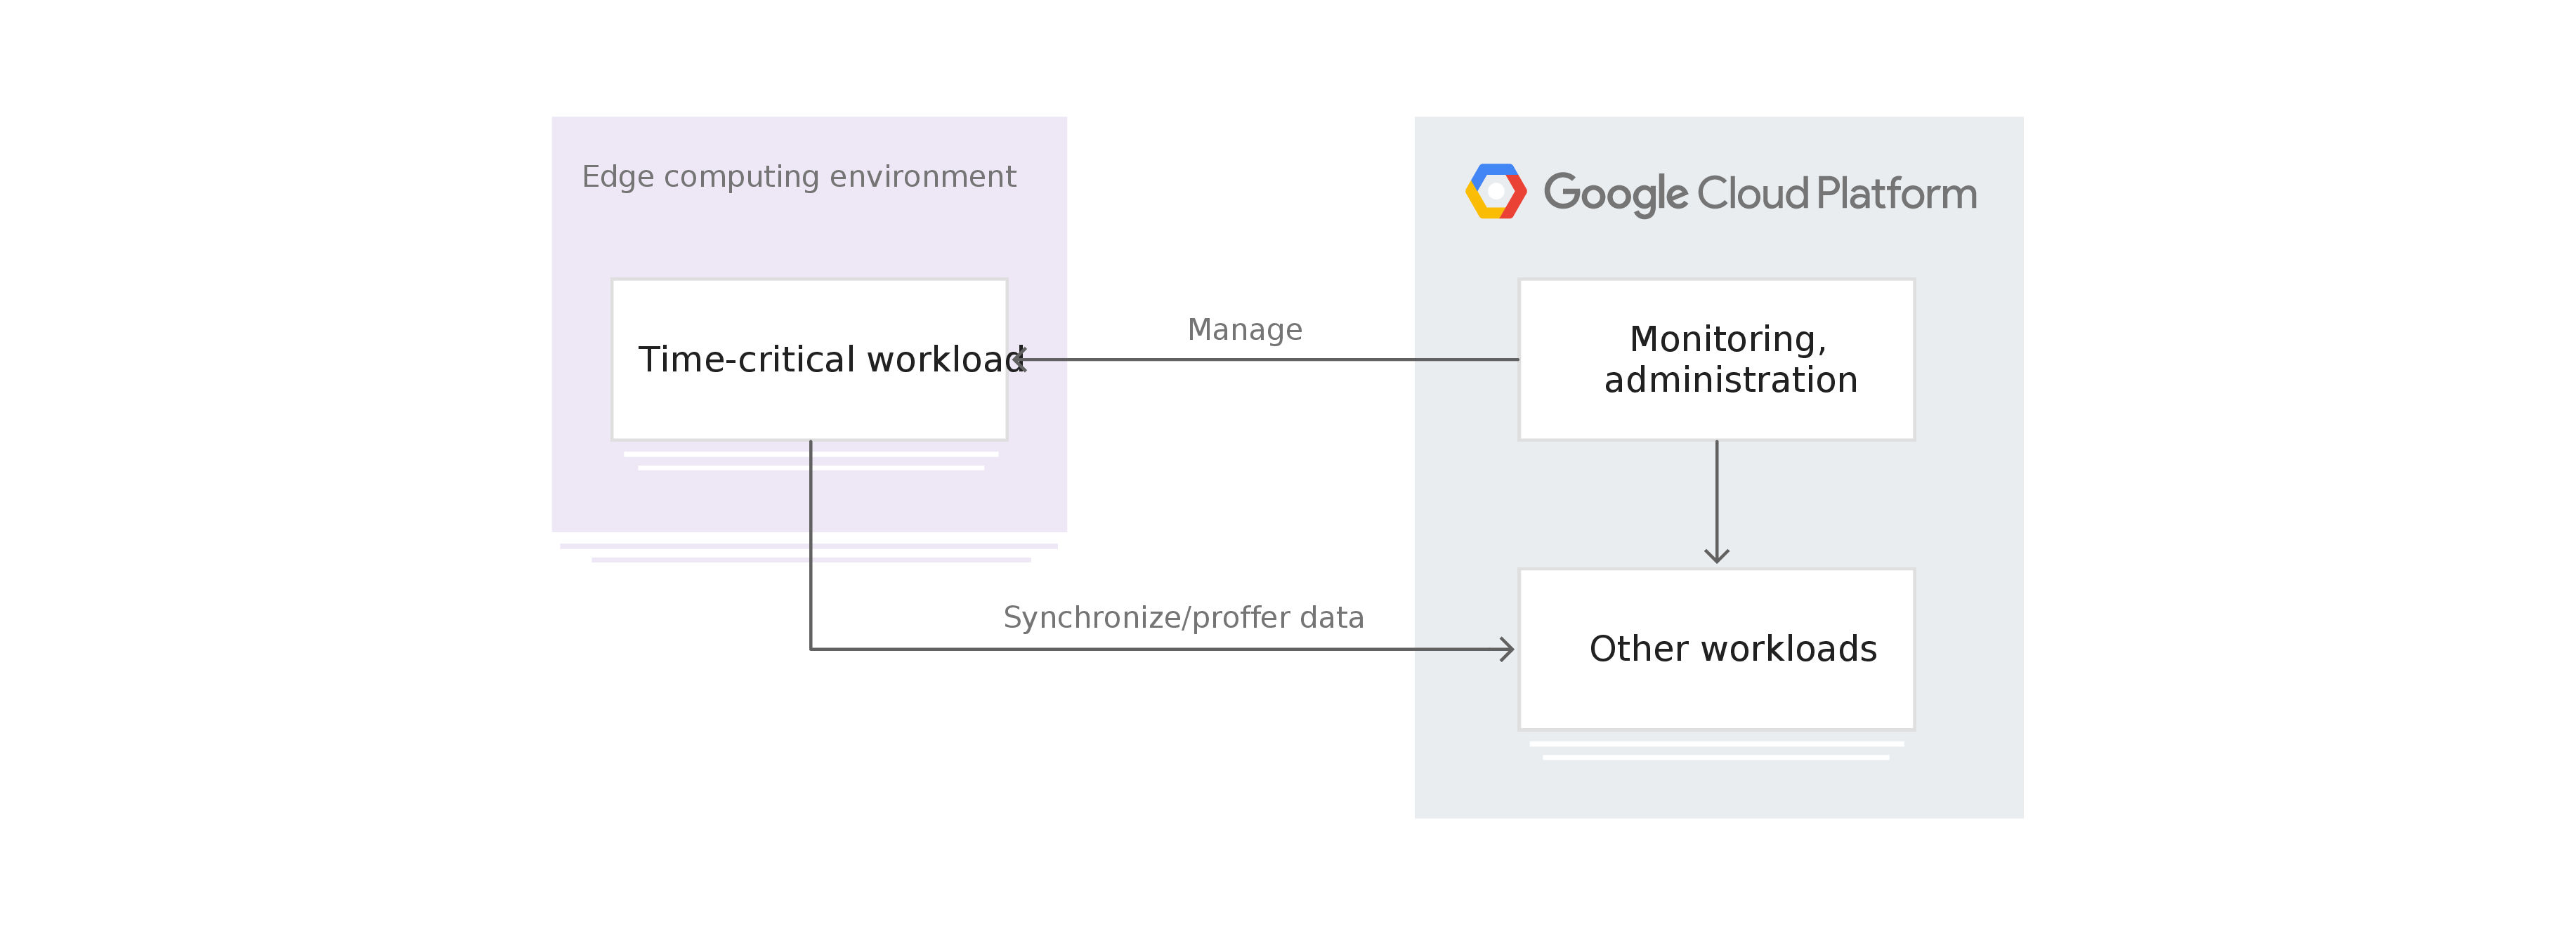
\includegraphics[width=0.8\textwidth]{images/edge.jpg}
    \par
	  \caption{Google Edge architektura\label{fig:edge}, zdroj: \source{\cite{edge-picture}}}
    \end{centering}
\end{figure}

Řešení pro správu hybrid cloud prostředí nabízí uživatelům možnost spravovat zdroje různých poskytovatelů z jednoho cetralizovaného místa. Některá řešení jako jsou Red Hat Cloudforms (Manage IQ) a Mist.io se zaměřují primárně na správu infrastruktury u jednotlivých poskytovatelů. Jejich úkolem je připravit infrastrukturu, kam patří fyzické a virtuální servery, uložiště a síťové prvky, pro běh aplikací napříč zdroji \linebreak od více poskytovatelů. Na druhé straně řešení jako Spinnaker, Kubernetes Federation a Cloud foundry se primárně zaměřují na správu aplikací, které běží distribuovaně \linebreak u více poskytovatelů cloudu. V následující sekci jsou jednotlivá řešení představena detailněji. 


\section{Red Hat Cloudforms/Manage IQ}
Cloudforms je platforma pro jednotnou správu fyzických a virtuálních serverů a také kontejnerů napříč různými cloudovými prostředími. Pomocí CloudForms je možné ovládat zdroje v technologiích pro privátní cloudy OpenStack a také virtuální servery spravované technologií od společnosti VMware, Red Hat virtualization a Microsoft Hyper-V. CloudForms umožňuje spravovat zdroje ve veřejných cloudech AWS (Amazon web services), Microsoft Azure a také GCP (Google cloud platform). CloudForms umožňuje spravovat také kontejnery na platformě OpenShift. CloudForms technologie vychází z Manage IQ technologie. Manage IQ je jednotná open-source platforma pro správu cloudových prostředí. Cloudform je vyvíjeno, spravováno a podporováno přímo společností Red Hat, jedná se o komerční řešení. Manage IQ je stejná platforma s otevřeným kódem, která je spravována a rozvíjena komunitou napříč různými společnostmi \cite{manageiq}. Dále v textu je popisována Manage IQ verze.\par
    Manage IQ přistupuje k jednotlivým systémům, označovaným jako poskytovatelé, přes API, které např. veřejné cloudy nebo OpenStack poskytují. Přes tato API si \linebreak Manage IQ vyčítá informace o jednotlivých zdrojích  jako jsou virtuální servery, kontejnery, load-balancery společně s jejich metadaty jako jsou jméno, typ a mnoho dalšího. Tyto zdroje jsou označovány jako managed elements, neboli spravovaný prvek, a jsou uloženy ve Virtual Managemet Database (VMDB). Manage IQ po počátečním získání informací z jednotlivých poskytovatelů stále sleduje jednotlivá API poskytovatelů a udržuje VMDB stále aktuální. Manage IQ poskytuje přehledné webové rozhraní ve kterém jsou zobrazeny jednotlivé zdroje poskytovatelů s detailními informacemi.\linebreak Například při připojení na VMware je zobrazen seznam běžících virtuálních serverů společně s jejich atributy jako je počet jader, velikost RAM, operační systém, připojené sítě, nainstalované programy a tak dále. \par
    Manage IQ dovoluje provádět akce nad objekty, které má zaregistrované ve VMDB. Například virtuální servery běžící ve VMware prostředí můžeme vytvářet, mazat, vypínat, zapínat a restartovat. Další oblastí správy zdrojů je sledování a provádění změn. Můžeme sledovat jednotlivé atributy zdrojů a také kdy došlo k jejich změně. Manage IQ umožnuje také porovnávat aktuální stav s počátečním stavem. Např. jaké změny byly provedeny na virtuálním serveru oproti jeho základní konfiguraci. Manage IQ může zaznamenat změnu sudo práv, přidání nového uživatele nebo nainstalování \linebreak nového balíčku. Protože Manage IQ má data o všech zdrojích jednotlivých poskytovatelů, můžeme s jeho pomocí počítat náklady na provoz.\par
    Další věcí, kterou Manage IQ nabízí jsou služby. Služby dovolují vytváření složitějších konfigurací jednoduchou cestou. Přes služby můžeme například vytvořit dva virtuální servery s nainstalovaným webovým serverem, jeden server poběží v prostředí OpenStacku a druhý na VMwaru. Dále virtuální server sloužící jako databáze a poté ještě load-balancer, který bude rozkládat zátěž mezi webové servery. Výběr těchto zdrojů může například sloužit vývojářům aplikace jako prostředí pro vývoj. Vytvořit takovéto prostředí bude možné na jedno kliknutí. Správce vytvoří podle požadavků skript, který tyto zdroje vytvoří a poté zdroje nastaví. Vývojáři mohou z webového rozhraní skript spustit a během chvíle dostanou připravené prostředí pro vývoj. Tento nástroj dovoluje vytvářet složitější konfigurace a jednoduše je nasadit. Vývojáři tak tráví více času programováním aplikace namísto nastavování serverů. Administrátoři mohou povolit přistup k určitým zdrojům pouze uživatelům, kteří splnují stanovená pravidla. Např. pouze uživatelé ve skupině vývojáři mohou spouštět skript, který vytvoří vývojářské prostředí z předchozího příkladu \cite{lwn}.

\section{Cloud foundry}
Cloud Foundry (CF) je open source cloudová PaaS platforma. Na této platformě mohou vývojáři jednoduše vytvořit, nasadit, běžet a škálovat aplikace. CF bylo původně vytvořeno společností VMware. Později došlo ke zveřejnění zdrojových kódů a stalo se komunitním projektem. Jedná se o Paas řešení, které je dobře nastavitelné a rozšiřitelné, uživatelé mohou používat širokou škálu frameworků a programovacích jazyků. CF může být nasazeno na vlastní hardware případně na jinou podporovanou cloud platformu jako je AWS nebo OpenStack. CF poskytuje seznam certifikovaných platforem jako jsou IBM Cloud Foundry, Atos Cloud Foundry nebo Pivotal Cloud Foundry. Tyto certifikované platformy zaručují, že aplikace se budou na těchto platformách chovat stejně. Tento fakt minimalizuje vendor lock-in, tedy upoutání se pouze na jednoho poskytovatele. Další výhodou je možnost využití CF pro provozování aplikací na více cloudech, tedy multi-cloud \cite{cf}.\par
CF se skládá z mnoha komponent a má otevřenou architekturu, které zahrnuje tkz. buildpack mechanismus. Tento mechanismus dovoluje přidávat nové frameworky, aplikační služby a také rozhraní pro cloudové poskytovatele. Prvním komponentou je router, který směruje příchozí požadavky na odpovídající komponenty. Další komponentou je UAA (user account and authentication) server, který vykonává správu identit obsažených v systému a přístup uživatelů k jednotlivým zdrojům. Další důležitou komponentou je Cloud Controller, který zajišťuje nasazení aplikace. Cloud controller řídí Diego Brain komponentu, aby spustila požadovanou aplikaci a společně obstarávají celý životní cyklus aplikace. Diego Brain je komponenta, která spouští jednotlivé aplikace a sleduje zda se aplikace nachází v požadovaném stavu. Diego Brain, implementuje control plane, rozhoduje o tom co a kde bude spuštěno. Pro samotné spuštění je zodpovědná komponenta Diego Cell. Cell jsou virtuální servery, na kterých běží požadované aplikace. Aplikace jsou spouštěny v kontejnerech. CF používá jako běhové kontejnerové prostředí vlastní produkt Garden-runC \cite{garden}, který splňuje OCI standard. Diego Cell poskytuje pro tyto kontejnery statistiky použití, logy a další informace. Další funkcí CF jsou služby. Služby fungují v CF jako katalog, ze kterého si vývojář vybírá. Příkladem může být MySql, Redis, Jenkins, Rabbit MQ a mnoho dalších. Vývojář může využít předem definované zdroje, které společně s jeho aplikací vytvoří vybranou službu, bez nutnosti manuální instalace a konfigurace daného nástroje. CF dovoluje vytvářet a přidávat vlastní služby. Aby mohly být služby uspěšně spuštěny, musí implementovat definované API \cite{pivotal}. \par
    Aby mohlo CF spouštět aplikace na virtuálních serverech, potřebuje ovládat infrastrukturu, která hostuje CF aplikace. K tomuto učelu slouží nástroj BOSH, který \linebreak zaručuje, že prostředí je správně nastavené a připravené hostovat uživatelské aplikace. BOSH se skládá ze tří vrstev. První vrstvou je Stemcell, který představuje univerzální operační systém, který abstrahuje aplikaci od operačního systému serveru, je stejný přes všechny poskytovatele a umožnuje jednotnou správu virtuálních serverů. Druhou vrstvou je vydání (Release), popisuje jaký software by měl být nasazen a jak by měl být nastavený. Druhá vrstva zaručuje opakované spuštění aplikace se stejným výsledkem. Poslední částí BOSH je 
    manifest soubor, který popisuje jaký release by měl být nasazený a do jakého cloudu. BOSH také dovoluje spouštět aplikace v multi cloud prostředí. BOSH používá Cloud provider interface (CPI), aby abstrahoval rozdíly mezi jednotlivými poskytovateli. Díky tomu je možné přidávat nové poskytovatele. BOSH v současnosti může nasadit aplikaci na platformy AWS, Azure, GCC, OpenStack a také VMware \cite{bosh}.

\section{Mist.io}
Mist.io je open-source platforma, která zjednodušuje uživatelům správu cloudu. Mist.io poskytuje jednotné rozhraní pro správu cloudových řešení různých společností. Nástroj Mist.io může spravovat fyzické servery, virtuální servery na technologiích KVM, \linebreak VMware, OpenStack nebo Rackspace. Mist.io ovládá také zdroje největších veřejných cloud poskytovatelů AWS, Google cloud engine a Azure. Mist.io dává uživatelům možnost monitorovat Docker kontejnery. Díky široké podpoře cloudových technologií může být Mist.io využito i pro správu multi-cloud infrastruktury a minimalizovat závislost pouze na jednom poskytovateli. Mist.io je možné využívat ve třech verzích. První verzí je Community edition, která je volně dostupná a uživatelé si ji musejí spravovat sami. Druhou verzí je Enterprise edition, která může být nasazena on premise na privátních serverech společnosti. Tato placená verze zahrnuje profesionální podporu od samotné společnosti Mist.io. Poslední možností je využítí SaaS verze Mist.io produktu. Uživatelé této verze platí pouze za využítí zdrojů a jedná se o nejjednodušší řešení jak s Minst.io začít. SaaS verze poskytuje stejně jako Enterprise edition profesionální podporu. Tato kapitola je vytvořena s využitím oficiální dokumentace k Mist.io nástroji \cite{mistio}.\par
    Mist.io poskytuje webové rozhraní pro správu a monitoring jednotlivých zdrojů \linebreak napříč různými poskytovateli. Součástí aplikace je i API, které umožnuje automatizovat jednotlivé postupy. Prvním krokem je přidání cloudových platforem, které budou \linebreak spravovány. Každý poskytovatel vyžaduje rozdílnou konfiguraci pro správné \linebreak fungování. Například pro správu fyzického serveru je nutné poskytnou ip adresu, ssh klíč, uživatele s root právy a číslo portu pro připojení. Pro připojení AWS poskytovatele je nutné vyplnit API klíč a přístupový klíč. Po přidání jednotlivých poskytovatelů je možné si prohlížet jednotlivé zdroje poskytovatelů a dále s nimi pracovat. Mist.io rozlišuje několik základních zdrojů jako jsou machines, images, networks, keys a scripts. Machines, neboli servery, jsou všechny fyzické a virtuální servery. Ve webovém rozhraní jsou servery jednotlivých poskytovatelů rozlišeny ikonkou. U serverů je možné si prohlížet jejich detaily jako je vytížení procesoru, využití RAM nebo \linebreak zaplněnost disků. Dále je možné spravovat pravidla definovaná pro daný server. \linebreak Pravidla umožnují definovat akci, která se má provést při splnění určitého pravidla. Například pokud služba na serveru neodpovídá, tak dojde k restartu služby. Jednotlivé servery je možné seskupovat do skupin podle tagů, neboli nálepek, a efektivně s nimi pracovat. Mist.io podporuje ssh připojení na vzdálený server přímo z webového prohlížeče. Každý server je možné ovládat pomocí definovaných akcí. Každý poskytovatel nabízí jinou sadu akcí, které je možné vykonávat. Mezi ty základní patří vypnutí, restart a smazání serveru. Jednotlivé servery pak mohou být vytvořeny přímo \linebreak ve webovém rozhraní nebo přes API. Při vytváření serveru je možné specifikovat jméno serveru nebo poskytovatele, ve kterém bude server spuštěn. Druhým zdrojem jsou images, které slouží pro vytváření serverů nebo kontejnerů. Mist.io zobrazuje \linebreak images, které objevil v jednotlivých public nebo private poskytovatelích a také z připojeného Docker engine. Součástí kontejner images jsou i základní Docker images, které poskytuje přímo Mist.io. Pro další zdroj networks, umožnuje Mist.io zobrazit sítě jednotlivých poskytovatelů společně s informacemi o nich a případně v nich vytvářet subnety.  Aby mohli uživatelé přistupovat přes webové rozhraní na konzoli serverů, Mist.io nabízí možnost spravovat ssh klíče, ty poté přiřazovat jednotlivým zdrojům a získat tak přístup na jejich konzoli. Pokud uživatel klíč nemá, může si ho přes webové rozhraní vytvořit. Posledním zdrojem, který Mist.io nabízí je script. Zdroj script slouží \linebreak k automatizaci opakujících se ukonů nebo konfiguraci serverů. Jednotlivé script zdroje mohou být vytvořeny v bashových skriptech nebo jako Ansible playbooks. 

\section{Kubernetes federation}
Některé nástroje na správu multi cloud prostředí implementují vlastní řešení jak spravovat Kubernetes clustery napříč různými lokacemi. Kubernetes komunita se také \linebreak rozhodla vyvinout řešení pro správu více clusterů, která je zajímavá pro spoustu \linebreak společností a přidává další možnosti využití. V porovnání s jedním clusterem je \linebreak nasazení aplikace do více clusterů komplikovanější. Jedním z problémů je, jak bude workload jednotlivých aplikací rozdělován do různých clusterů. Existuje několik \linebreak možností, replikovat zdroje aplikace mezi všechny clustery, replikovat pouze mezi vybrané clustery nebo zdroje rozdělit mezi jednotlivé clustery. Dále je nutné vyřešit jak bude řízen přistup k jednotlivým clusterům nebo jak postupovat, jestliže vytvářené zdroje nebo jejich část již v nějakém clusteru existují. První verze řešení označovaná jako v1 využila koncept Kubernetes API, aby odstranila jakoukoliv přidanou složitost pro existující uživatele k8s. Tento přístup ovšem nebyl proveditelný, protože zahrnoval spoustu problémů jako jsou složitost při znovuvytváření k8s api na úrovní clusteru, omezená flexibilita ve federovaných typech. Jedním z problémů byla také neustálená cesta ke stabilní veřejné dostupnosti (GA verze) a zmatek ohledně k8s API samotného. Například k8s deploymenty jsou veřejně dostupné v Kubernetes projektu, ale ve v1 verzi Kubernetes federace nebyly dostupné ani v beta verzi. \par
    Původní myšlenka s federací specifické API architektury se dále rozvinula a v současnosti pokračuje jako verze v2. Zatím se jedná pouze o Alfa verzi, která není doporučená používat pro produkční použití. Nový návrh architektury je zobrazen na obrázku \ref{fig:k8s-federated}. Federace může být nastavena pomocí dvou typů informace. Prvním typem je Type configuration, který nám říká, jaké zdroje v API má federace propagovat. Druhým typem je Cluster configuraton, která určuje do kterých clusterů má federace propagovat jednotlivé zdroje. Informace Type configuration se skládá ze tří částí. Template, neboli šablona, obsahuje základní konfiguraci zdroje. Například zdroj FederationReplicaSet obsahuje informace o zdroji ReplicaSet, který má být distribuován do určených clusterů. Druhou částí je Placement, neboli umístění, který říká v jakých clusterech má být zdroj spuštěn. Poslední částí jsou Overrides, které určují specifické parametry pro jednotlivé clustery. Tyto tři části obsahují nejnutnější informace potřebné pro propagaci a jsou navržené tak, aby splňovaly dynamické plánování spouštění zdrojů založené \linebreak na pravidlech. Další důležité součásti federace k8s jsou Status, Policy a Scheduling. Status shromažduje informace o všech zdrojích spuštěných napříč všemi federovanými clustery. Policy, neboli politiky, rozhodují do jakých clusterů mohou být jednotlivé zdroje distribuovány. Scheduling, neboli plánování, zajišťuje rozdělení jednotlivých workloadů přes různé clustery co nejlépe a nejefektivněji.\par 
        Funkce, které by Kubernetes federace měla poskytovat patří propagace různých typů zdrojů do vzdálených clusterů, CLI nástroj kubefed2 pro správu takovéto federace podobně jako nástroj kubectl, který slouží pro správu jednoho clusteru. Federace by také měla poskytovat DNS a Ingerss služby pro více clusterů. Další funkcí by také mělo být pokročilé nastavení rozmístění jednotlivých zdrojů do clusterů podle uživatelovi preference.


\begin{figure}[H]
  \begin{centering}
	  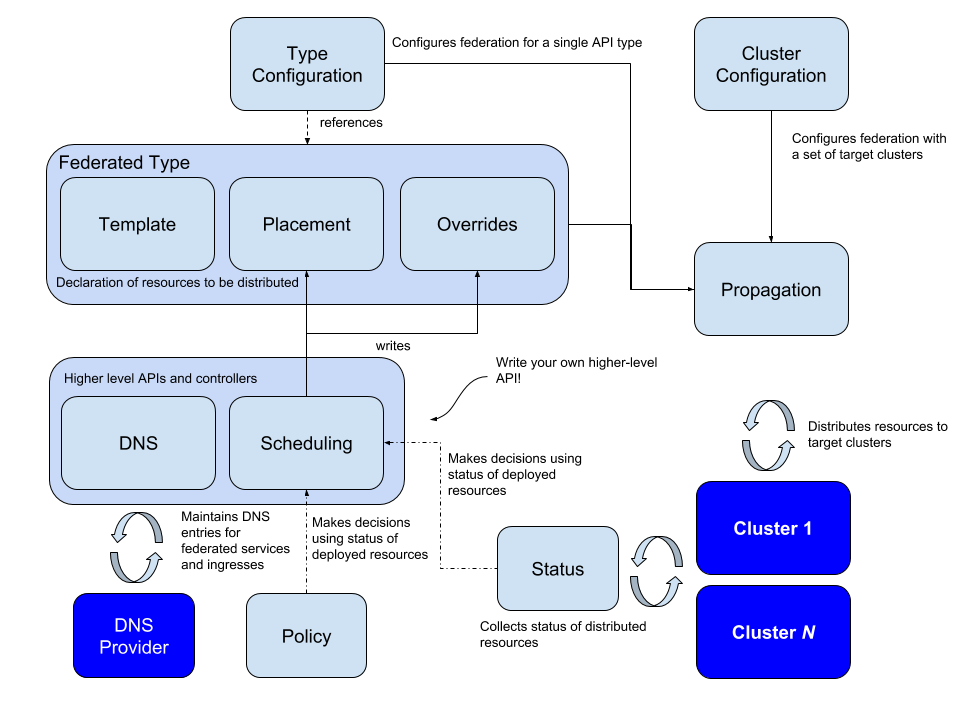
\includegraphics[width=0.8\textwidth]{images/k8s-federated.png}
    \par
	  \caption{Architektura projektu Kubernetes Federation\label{fig:k8s-federated}, zdroj: \source{\cite{federace-picture}}}
    \end{centering}
\end{figure}
	
\section{Spinnaker}
Spinnaker je open source platforma, která umožňuje continuous delivery (CD) aplikací do multi-cloud prostředí. Spinnaker projekt byl vytvořen společností Netflix. Spinnaker je navržen s ohledem na snadnou rozšiřitelnost tak, aby bylo možné přidávat nové cloudové poskytovatele. Spinnaker podporuje nejpoužívanější cloudové poskytovatele jako jsou AWS, Google Cloud, Azure, OpenStack, Oracle Cloud Infrastructure a také technologii Kubernetes \cite{netflix-spinnaker}. Mezi uživatele Spinnakeru patří například Waze, navigační aplikace pro mobilní telefony. Provozovatelé aplikace používají pro běh své aplikace AWS a Google cloud poskytovatele pro vysokou dostupnost své služby a také pro možnosti, které Spinnaker nabízí. Postup, který Waze používá začíná odesláním změn do github repozitáře, Jenkins software vytvoří balíček s požadovanou změnou a spustí další proces, jehož úkolem je nasazení aplikace. V obou cloudech zároveň je vytvořena image s požadovným balíčkem a jsou spuštěny integrační testy. Pokud testy proběhnou bez problémů, aplikace je spuštěna v tesovacím prostředí s reálnými daty. Jestliže aplikace v testovacím prostředí prošla testy je nasazena do produkčního prostředí. V případě chyby může být nová verze stažena z produkce a místo ní nasazena starší stabilní otestovaná verze \cite{waze}.\par
Spinnaker obsahuje dvě základní sady funkcí správu aplikací a nasazení aplikací. S pomocí správy aplikací je možné spravovat a monitorovat zdroje v jednotlivých \linebreak cloudech. Spinnaker vidí aplikace jako jednotlivé mikroslužby a takto s nimi pracuje. Spinnaker používá k popsání uživatelské aplikace, aplikace kterou chceme pomocí Spinnakeru nasadit do prostředí cloudu, koncepty jako jsou Applications, Clusters a Server Groups. Spinnaker dále používá koncepty Load balancer a Firewall pro popsání, jak budou jednotlivé mikroslužby zpřístupněny uživatelům. Koncept Application je ve Spinnakeru reprezentace mikroslužby uživatelské aplikace, její konfigurace a infrastruktury na které bude aplikace provozována. Ač to Spinnaker nevyžaduje, dobrou praxí je vytvoření Spinnaker aplikace pro každou mikroslužbu uživatelské aplikace. Pojem Cluster je označení pro skupinu serverů ve Spinnakeru. Server Groups označení používá Spinnaker pro nasaditelné zdroje jako jsou obrazy virtuálních serverů nebo Docker image a konfiguraci (počet instancí zdroje, metadata, pravidla pro škálování, atd.). Pokud je Server Group nasazena, je kolekcí instací dané mikroslužby (virtuální servery, pody v Kubernetes). Load balancer je použitý pro směrování požadavků mezi instance v jedné Server Group. Load balancer umí také kontrolovat dostupnost \linebreak mikroslužby a v případě poruchy přestat posílat požadavky na poškozený Server Group.\par
Druhá skupina funkcí, kterou Spinnaker nabízí se týká nasazení aplikace a CD (continuous delivery) aplikace. Hlavní částí nasazení aplikace je Pipeline. Pipeline se skládá z posloupnosti akcí, které se označují jako Stages. Pipeline je možné spustit ručně nebo lze nastavit spouštěče. Jako spouštěč mohou být nastaveny různé podněty jako je nový Docker image v Docker registry, dokončení Jenkins úlohy, časový údaj atd. Pipeline také může uživatele upozorňovat o svém spuštění, průběhu, dokončení nebo chybovém hlášení. Stage je atomická část Pipeliny. Jednotlivé Stage se dají různě skládat. Například některá Stage musí být úspěšně dokončena předtím než je spuštěna další. V jiném případě může být spuštěno více Stagí najednou. V rámci jedné Stage může být vytvořen balíček s aplikací, vytvořen Docker image, spuštění testů aplikace nebo  spuštění virtuálního serveru s novou verzí aplikace. Spinnaker využívá cloud native strategie pro správu aplikací. Mezi tyto strategie patří ověřování dostupnosti služeb, nasazení nové verze aplikace společně s blue/green a canary testováním a také možností vrátit předchozí verzi aplikace bez větších komplikací \cite{spinnaker}.


\chapter{Návrh a implementace systému pro běh distribuovaných aplikací}
\section{Definice požadavků na běh distribuované aplikace}
V předchozí kapitole jsou představeny projekty, které řeší otázku jak spravovat jednotlivá cloudová řešení a aplikace napříč různými cloudovými poskytovateli co nejefektivněji z jednoho místa. Současným trendem jak provozovat aplikace v prostředí cloudu je využití kontejnerizace a nástroje Kubernetes pro správu těchto kontejnerů, viz. kapitola Cloud native. Kubernetes architektura a nástroje pro správu K8s jsou navrženy pouze pro provozování jednoho clusteru. Mnoho společností se zajímá o propojení jednotlivých clusterů tak aby tvořily jeden celek. Tento přístup přináší mnoho výhod. Uživatelé mají možnost spravovat několik clusterů z jednoho místa. Z tohoto centrálního uzlu by uživatelé měli být schopni vytvářet zdroje v jednotlivých clusterech a také odtud sledovat chování a stav jednotlivých clusterů. Další výhodou je využití několika poskytovatelů pro lepší dostupnost svých služeb. Při výpadku jednoho poskytovatele máme pořád běžící aplikaci u druhého poskytovatele. Dalším použitím více clusterů je Edge cloud koncept. K8s clustery, umístěné v místě potřeby snižují odezvu na události a zvyšují dostupnost pro kritické aplikace. Propojením jednotlivých k8s clusterů se zabývá spousta společností a také k8s komunita. Konkrétně se jedná o projekt Kubernetes Federation, který je představen v předchozí kapitole.
     Správa více k8s clusterů je komplexní úkol a musí splňovat několik požadavků, aby bylo možné jednoduše a z jednoho místa efektivně provozovat distribuovanou aplikaci: 
\begin{itemize}
\item První požadavkem takového systému je možnost jednotně spravovat desítky až tisíce k8s clusterů. Systém by měl nabízet jeden vstupní bod pro obsluhu všech k8s clusterů z jednoho místa.  Manuálně spravovat jednotlivé clustery není \linebreak výhodné, protože toto řešení špatně škáluje. Pokud se například společnost, \linebreak využívající edge cloud v každé pobočce, bude rozrůstat o nové pobočky, bude muset pro každé dvě až čtyři pobočky zaměstnat nového operátora k8s clusteru. Efektivnějším řešením je definovat aplikaci v centrálním systému a poté podle potřeby distribuovat danou aplikaci na jednotlivé clustery. Výhodou použití k8s v jednotlivých lokacích je stejné a konzistentní prostředí přes všechny clustery. Odpadá tak nutnost ovládat technologie od různých společností. Spouštění a provozování aplikací bude v jednotlivých lokacích probíhat stejně jako v testovacím prostředí. Pro doručování nových verzí aplikace, nabízí k8s tkz. rolling updates. Tato funkce umožňuje bezvýpadkové nahrání nové verze aplikace. K8s postupně nahrazuje pody se starou verzí aplikace, jeden po druhém a zároveň spouští pody s novou verzí. Nové funkce a opravy tak mohou být rychleji aplikovány. Pokud dojde k nahrání špatné verze aplikace, která nebude fungovat, k8s umožní se rychle vrátit na předchozí funkční verzi. 
\item     Dalším plusem je použití k8s architektury a všech zdrojů a technik, které k8s nabízí. K8s je robustní nástroj, který v sobě zahrnuje vysokou dostupnost, škálovatelnost, rozšiřitelnost, je to řešení odolné vůči chybám, vyvíjené, spravované a podporované širokou komunitou. Pro zmíněné atributy se k8s stalo de facto standardem pro orchestraci kontejnerů. Například použití Pod konceptu, namísto kontejneru. Pod dovoluje seskupit více kontejnerů, které na sobě úzce závisí a potřebují být spuštěny na stejném serveru nebo mezi sebou sdílejí zdroje, do jednoho logického celku. Pod dovoluje také využití tkz. Side-car konceptu. Side-car je označení pro kontejner, který běží ve stejném podu jako kontejner uživatelské aplikace a poskytuje další služby jako je sběr logů z uživatelského kontejneru a jejich odeslání na centrální server. 
\item Pro přístup více subjektů do systému je nutné izolovat zdroje jednotlivých subjektů tak, aby na sebe vzájemně neviděly a nemohly tak ovlivňovat aplikace ostatních zákazníků. Pro tento problém poskytuje k8s namespace. Namespace je virtuální cluster uvnitř fyzického clusteru. Jednotlivé zdroje uvnitř namespace jsou izolovány od ostatních. Uživatelé jsou schopni vytvářet, prohlížet, upravovat a mazat pouze zdroje v přiděleném namespacu. Namespace může být využit pro oddělení jednotlivých aplikací, různá oddělení jedné společnost mohou mít vlastní namespace, případně různé firmy mohou být odděleny pomocí namespacu. 
\item Dalším požadavkem je spuštění různých aplikací v clusterech situovaných \linebreak v různých lokacích. Např. aplikace, kterou zákazníci v obchodě používají pro výběr zboží budeme provozovat ve všech obchodech. Aplikaci pro interní zaměstnance, která ulehčuje správu skladů se zbožím budeme provozovat ve všech skladech a také v největších obchodech s vlastním skladem. Pro tento učel je možné využít labely, neboli popisky jednotlivých objektů. Labels v k8s mají \linebreak podobu klíč a k němu přiřazená hodnota. Jednotlivé k8s deploymenty je možné popsat labely clusterů, ve kterých má být daný deployment spuštěný. Aplikace pro zákazníky by tak mohla obsahovat label lokace:praha a label typ:prodejna. Pomocí labelů je tak možné jednoznačně určit lokace a typ prodejny na které má být aplikace spuštěna. 
\item Důležitým aspektem pro běh distribuovaných aplikací je řízení přístupu uživatelů k jednotlivým zdrojům. K8s obsahuje několik mechanismů pro ověření zda uživatel má právo provést danou akci či nikoliv. Administrátoři tak mohou kontrolovat jaké akce mohou uživatelé vykonávat. Více o problematice a typech k8s autorizace je uvedeno v \cite{k8sauth}.
\end{itemize}

\section{Návrh aplikace}
V následující kapitole je popsána architektura systému, který umožňuje běh cloud native aplikací v k8s clusterech podle požadavků definovaných v předchozí kapitole \linebreak Definice požadavků na běh distribuované databáze. Architektura systému je zobrazena na obrázku \ref{fig:vk8s-architecture}. Systém se skládá ze tří menších celků. Prvním část se skládá z Kubernetes API a databáze Etcd. Uživatelé interagují s touto částí, s jejíž pomocí vytvářejí zdroje, které jsou dále distribuovány do jednotlivých clusterů. Druhá část systému se stará o distribuci uživatelských zdrojů do zvolených clusterů. Tato část se nazývá Controller. Třetí část je tvořena k8s clustery, které jsou umístěné v různých lokacích a zajišťují běh zvolených aplikací.\par
První část, která se skládá pouze z k8s API a Etcd databáze, je vstupní bod pro uživatele, kteří budou vytvářet své aplikace. Tento koncept je převzatý z k8s Master serveru, ovšem bez služeb Controller Manageru a Scheduleru. K8s API umožnuje vytvářet nové definice zdrojů a manipulaci s nimi. Konfigurace je uložena v databázi Etcd. Uživatelé mohou použít existující řešení pro správu k8s zdrojů jako je webové rozhraní k8s nebo nástroj kubectl pro správu k8s z příkazového řádku. Tyto nástroje umožňují také monitorování jednotlivých zdrojů. Na obrázku můžeme vidět, že Customer 1 vytvořil v přiděleném namespacu Deploymenty D1, D2, D3. Každý Deployment se skládá z N kontejnerů, které jsou označeny Pn. Zdroje, které se nachází v tomto centrálním API budou nazývány jako virtuální zdroje. Například virtuální Deployment D1 prozatím existuje pouze v centrálním API v podobě předpisu jak by měl být spuštěn a provozován. API také obsahuje mechanismy pro autentifikaci uživatelů na základě definovaných pravidel. Pro oddělení zdrojů jednotlivých uživatelů jsou použity namespacy. Uživatelé tak budou moci pracovat pouze se zdroji v přiděleném namespacu. Tento přístup zajistí bezpečný a izolovaný přístup více uživatelů do systému. Jak je zobrazeno na obrázku, Customer 1, má možnost spravovat pouze zdroje v zeleném namespacu a nikdy nemá možnost interagovat se zdroji Customera 2 v oranžovém namespacu a naopak.\par
Úlohou Controlleru je distribuovat zdroje z centrálního API serveru do jednotlivých clusterů v různých lokacích podle definovaných pravidel. Controller sleduje databázi zdrojů v centrálním API. Pokud uživatel vytvoří nový Deployment, Controller zjistí tuto skutečnost a podle labelů, které jsou přiřazené tomuto Deploymentu vloží konfiguraci Deploymentu do k8s clusterů v požadovaných lokacích. Jak můžeme vidět na obrázku, všechny tři Deploymenty uživatele Customer 1 jsou spuštěny ve všech třech dostupných lokacích. Tato strategie je nejjednodušší. Deploymenty zákazníka Customer 2 jsou spuštěny pouze ve dvou ze tří lokací, konkrétně v New Yorku a Praze. Zákazník Customer 2 například nemá pobočku v Londýně a proto nepotřebuje spouštět aplikaci v tomto regionu. Customer 2 má ovšem možnost v budoucnu spustit svou aplikaci v lokaci Londýn pokud to bude potřebovat. Uživatel tak přes centrální API přidá label, který popisuje lokaci v Londýně. Tuto změnu Controller zjistí a vloží definici \linebreak do k8s clusteru v lokaci Londýn. Controller také podporuje spustit v lokaci Londýn pro uživatele Customer 2 pouze Deployment D1. Proto aby uživatelé mohli monitorovat své zdroje z centrálního API, Controller sleduje k8s clustery v jednotlivých lokacích a zpět do centrálního API vkládá informace o jednotlivých zdrojích. Uživatelé tak například vidí stav jednotlivých podů a další informace o Deploymentech.\par
V jednotlivých lokacích je spuštěn plnohodnotný k8s cluster. Tento cluster spouští aplikace podle konfigurace, kterou obdžel od Controlleru. Jednotlivé clustery jsou samostatné rozhodovací jednotky, které jsou na sobě nezávislé. Při výpadku spojení na centrální API, aplikace běžící v clusteru stále fungují a mohou tak obsluhovat uživatele. Po obnovení spojení jsou data o aplikacích nahrána zpět do centrálního API. 

\begin{figure}[H]
  \begin{centering}
    
	  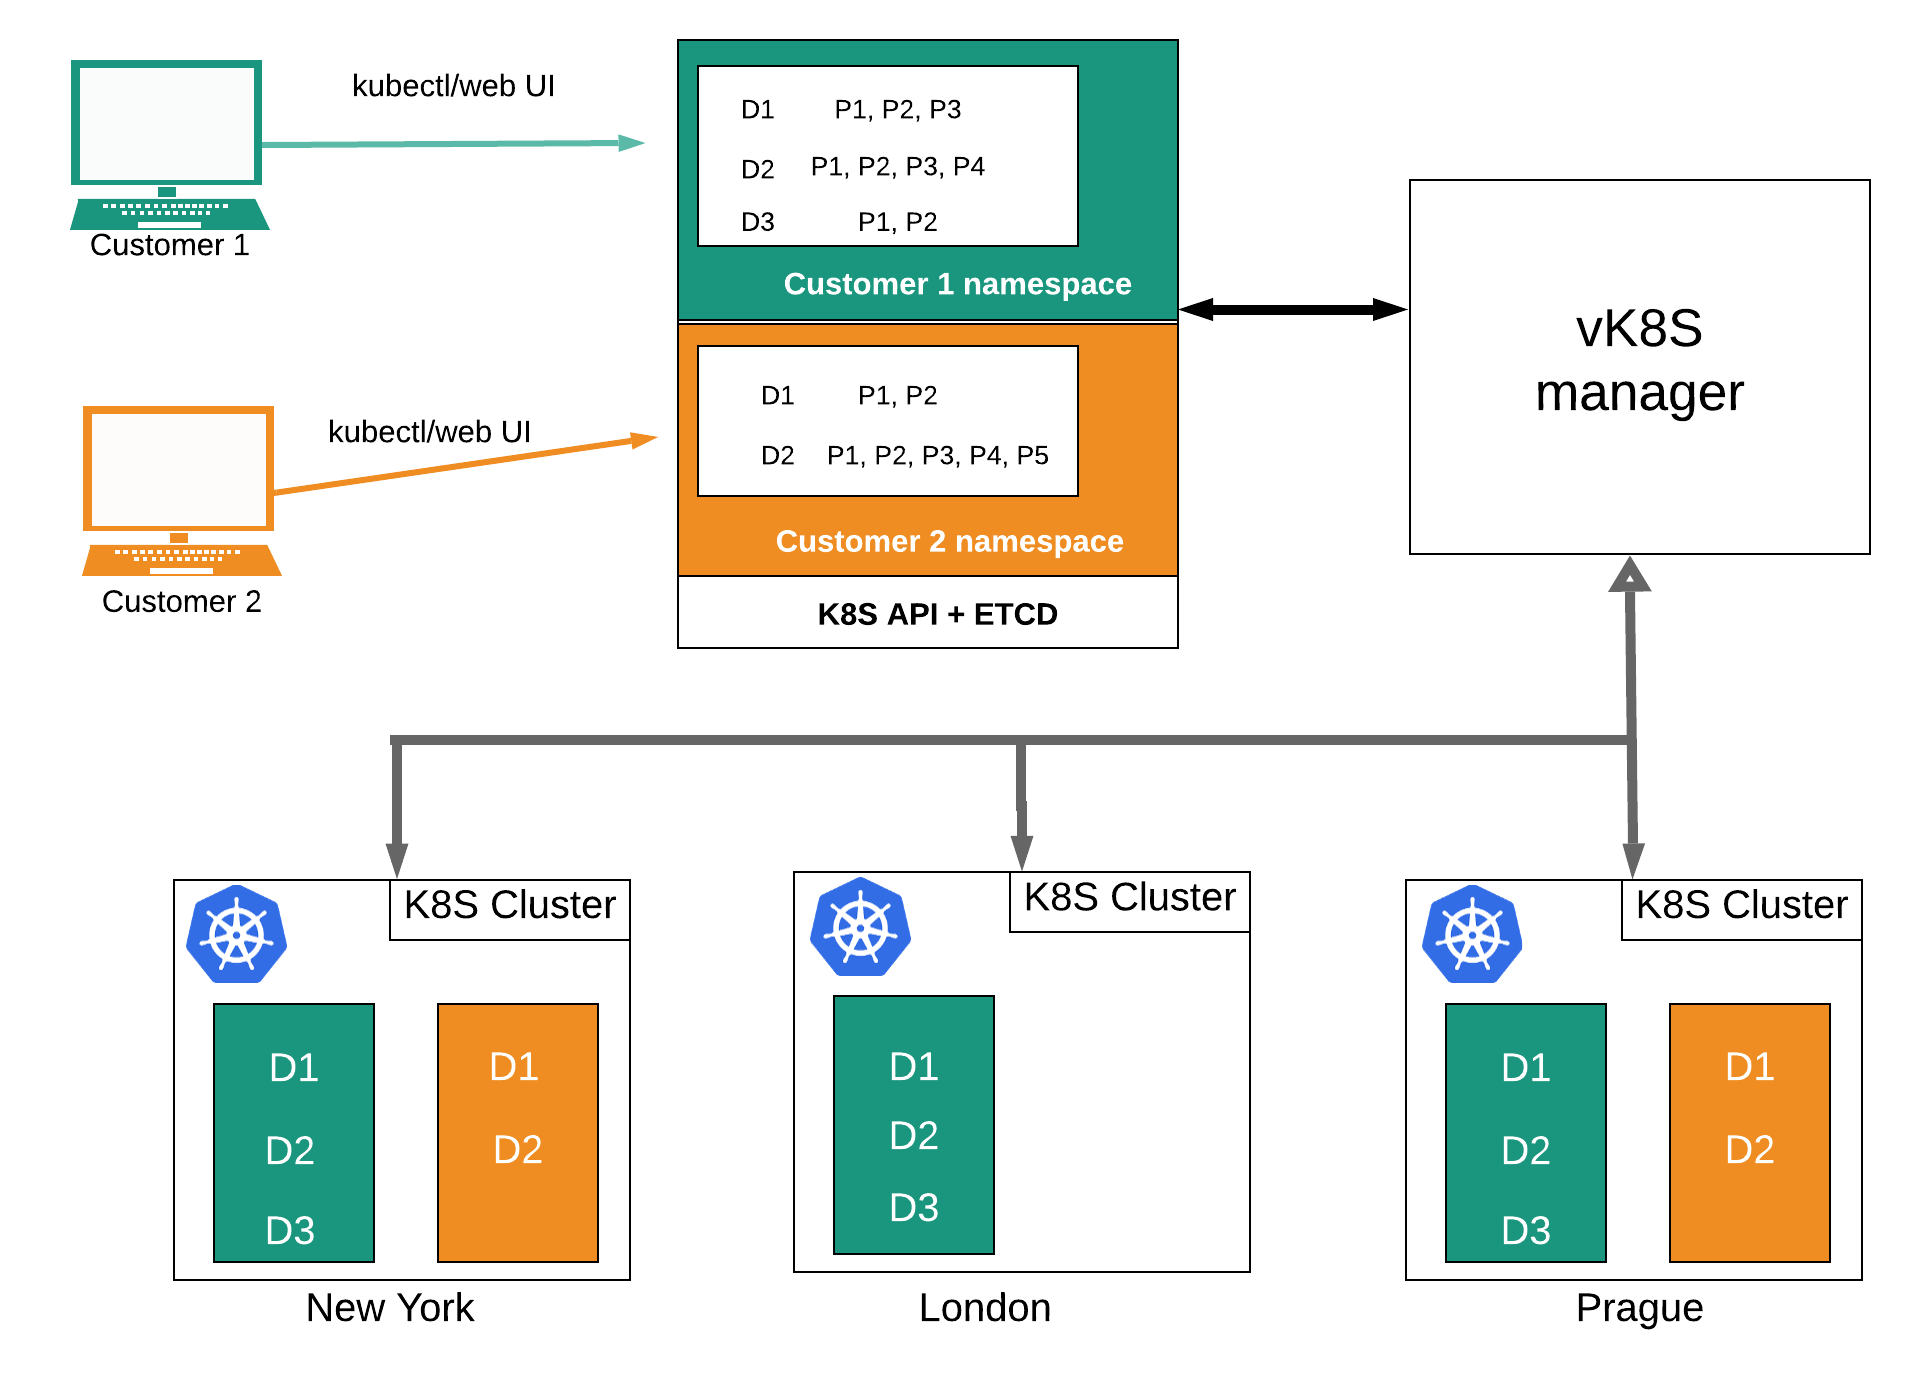
\includegraphics[width=0.8\textwidth]{images/vk8s-architektura.png}
    \par
	  \caption{Architektura navrhované aplikace\label{fig:vk8s-architecture}, zdroj: vlastní tvorba}
    \end{centering}
\end{figure}

\section{Implementace prototypu aplikace}
V předchozí kapitole je představena architektura systému, který umožňuje běh aplikací napříč více Kubernetes clustery. V této kapitole je představen prototyp aplikace, která tuto architekturu implementuje. Pro pojmenování jednotlivých částí aplikace jsou použity pojmy definované v architektuře aplikace. Pro vytvoření aplikace byl použit programovací jazyk Golang, zkráceně Go. Go programovací jazyk byl vytvořen zaměstnanci společnosti Google v roce 2009. Go je kompilovaný staticky typovaný jazyk, který umožňuje překlad zdrojových kódů do strojového kódu. Go se snaží být jednoduchý a dobře čitelný programovací jazyk. Go obsahuje na paměť nenáročná vlákna, nazývaná goroutines, které umožňují bez větších problémů v aplikacích spustit stovky až tisíce takovýchto goroutines. Pro komunikaci mezi jednotlivými goroutinami poskytuje jazyk Go tkz. Channely. Dalším plusem jazyka Go je rychlá kompilace, stejně jako běh samotné aplikace. Go obsahuje silnou typovou kontrolu a automatickou správu paměti. Součástí specifikace jazyka Go je i jednotný formát kódu. Pro formátování nabízí jazyk nástroj gofmt. Jazyk plně podporuje UTF-8 kódování a je plně open source \cite{miek}. V jazyce Go je vytvořeno mnoho projektů například Docker nebo Kubernetes. I tento fakt je jedním z důvodů proč byl vybrán právě jazyk Golang. Kubernetes nabízí pro jazyk Go klientské knihovny, které dávají vývojářům možnost jak pracovat s Kubernetes API.\par
    Na obrázku \ref{fig:vk8s} je zobrazena komunikace jednotlivých částí aplikace. Customer \linebreak manager sleduje Customer API, složené z k8s API a Etcd databáze, ke kterému přistupují jednotliví uživatelé a vytvářejí v něm zdroje. Pokud Customer manager zjistí vytvoření nového zdroje, vytvoří událost, která tuto akci reprezentuje. Tato akce je zaslána \linebreak Minikube manageru s využitím channelu. Minikube manager obdrží tuto událost a provede stejnou akci v Minikube clusteru. Příkladem takovéto akce může být vytvoření Podu s jedním kontejnerem uvnitř. Uživatel vytvoří definici Podu v Customer API. Customer manager zjistí tuto událost a zašle definici Minikube manageru. Minikube manager přijme z channelu akci a vytvoří tuto definici v k8s clusteru. V tomto clusteru je podle definice spuštěn Pod. Minikube manager sleduje Minikube cluster a odesílá informace. Například Minikube manager odesílá přes channel 1 Customer manageru informace o stavu vytvořeného Podu, který aplikuje tyto informace do Customer API. Uživatel tak vidí informace o podu v Customer API stejně jako by se připojoval přímo do Minikube clusteru.\par


\begin{figure}[H]
  \begin{centering}
    
	  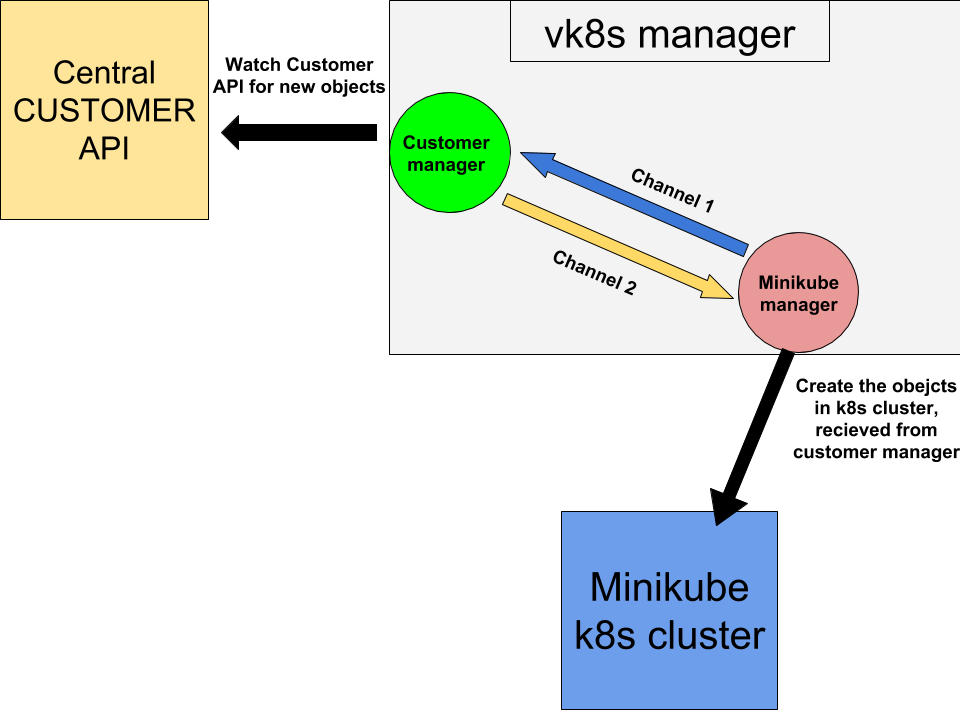
\includegraphics[width=0.8\textwidth]{images/vk8s.png}
    \par
	  \caption{Schéma vk8s manageru\label{fig:vk8s}, zdroj: vlastní tvorba}
    \end{centering}
\end{figure}

Zdrojový kód aplikace je dostupný v GitHub repozitáři\footnote[1]{\url{https://github.com/casek14/vk8s-manager}}. Struktura aplikace je uvedena v příloze \hyperref[app:struktura]{D}. Funkcionalita aplikace je rozdělena do jednotlivých balíčků (packages). Soubor main.go obsahuje instrukce jak se má aplikace spustit. Jako první je vytvořen objekt Manager, který se skládá ze dvou dalších částí. Manager je součástí balíku cluster. Jedna část, nazývaná Customer manager slouží pro interakci s centrálním k8s API. Druhou částí je Minikube manager, který interaguje s k8s clusterem. Funkce implementující vytvoření nového Managera je zobrazena na ukázce kódu \ref{lst:cluster}. Nejdříve jsou definovány jména namespaců, které budou dále využity. Poté jsou \linebreak vytvořeny dva managery, Customer Manager a Minikube Manager. Pokud vytvoření proběhlo úspěšně, metoda vrátí strukturu Manager. 

\begin{lstlisting}[caption={funkce vytvoření nového managera},label=lst:cluster]
func New() *Manager {
	log.Println("Preparing new Manager")
	customerNamespace := "mynamespace"
	customerName := "customer1"
	minikubeNamespace := fmt.Sprintf("%s-%s", customerNamespace, customerName)
	m, err := vk8s.New(&manager.Config{KubeConfigPath: minikubeKubeconfig, Namespace: minikubeNamespace, Mode: manager.Minikube})
	if err != nil {
		log.Fatalf("Unable to setup new manager, %s", err)
	}
	c, err := vk8s.New(&manager.Config{KubeConfigPath: customerKubeconfig, Namespace: customerNamespace, Mode: manager.Customer})
	if err != nil {
		log.Fatalf("Unable to setup new manager, %s", err)
	}
	return &Manager{m, c}
}
\end{lstlisting}
\par
											Implementace výše zmíněných Managerů se nachází v balíčku vk8s. Funkce \linebreak vk8s.New() v ukázce kódu \ref{lst:new} přijímá jako vstupní parametr strukturu Config z balíčku manager. Tato Config struktura obsahuje informaci o cestě k souboru kubeconfig, název namespacu a hodnotu Mode. Kubeconfig soubor se používá pro připojení a komunikaci s k8s API, obsahuje například ip adresu pro připojení k serveru nebo certifikáty k autorizaci. Hodnota Mode určuje zda bude vytvořen manager pro centrální customer API nebo pro k8s cluster minikube.\par 
\begin{lstlisting}[caption={vk8s.New() funkce pro vytvoření customer a minikube managera},label=lst:new]
func New(cfg *manager.Config) (manager.Interface, error) {
  if cfg.Mode == "" || cfg.Namespace == "" || cfg.KubeConfigPath == "" {
    return nil, fmt.Errorf("could not create new manager, incomplete configuration")
  }
  log.Printf("Preparing new %s manager", cfg.Mode)
  rc, err := k8s.NewRestConfig(k8s.Config{ConfigType: k8s.OutCluster, KubeConfigPath: cfg.KubeConfigPath})
  if err != nil {
    return nil, fmt.Errorf("Could not initialize rest config, err: %s", err)
  }
  clientset, err := kubernetes.NewForConfig(rc)
  if err != nil {
    return nil, fmt.Errorf("Could not initialize clientset, err: %s", err)
  }
  inf := informer.New(string(cfg.Mode))
  switch cfg.Mode {
    case manager.Customer:
      return &customer{vk8s{clientset, worker.New(clientset, inf), k8s.NewNamespaceObjectFromObject(clientset, &v1.Namespace{ObjectMeta: metav1.ObjectMeta{Name: cfg.Namespace}}), inf}}, nil
    case manager.Minikube:
      return &minikube{vk8s{clientset, worker.New(clientset, inf), k8s.NewNamespaceObjectFromObject(clientset, &v1.Namespace{ObjectMeta: metav1.ObjectMeta{Name: cfg.Namespace}}), inf}}, nil
    default:
      return nil, fmt.Errorf("unknown manager mode")
  }
}
\end{lstlisting}

Zmíněné managery implementují rozhraní manager.Interface, které obsahuje jednu metodu Start(inEvent, outEvent), která přijímá dva channely jako vstupní parametry. Na ukázce kódu \ref{lst:customer} je zobrazena metoda Start() pro Customer manager. Na začátku běhu funkce je ověřeno, že existuje potřebný namespace v customer API. Pokud neexistuje tak je vytvořen. V dalším kroku je vytvořen servisní účet, který bude aplikace používat pro práci s k8s API. Po vytvoření servisního účtu je spuštěna metoda Watch(outEvent), která sleduje zdroje v centrálním customer API a je detailně popsána dále v textu. Posledním krokem funkce Start() je sledování akcí na vstupním channelu. Slovo go před definicí funkce značí, že funkce bude spuštěna v goroutině, neboli \linebreak na paměť nenáročném vlákně. Uvnitř goroutiny se v nekonečném cyklu čeká \linebreak na události, které jsou obdrženy z inEvent channelu. Channely v jazyce Go fungují pro komunikaci mezi goroutinami. V tomto případě jedna goroutina do channelu zapisuje data a druhá z tohoto channelu data čte. Pokud na channelu přijde nějaká událost, je tato událost předána do volání funkce Run(), která tuto událost aplikuje do customer API. Například vytvoření nového zdroje je reprezentováno jako struktura Event s typem události Create a objekt, který má být vytvořen. Do inEvent channelu zapisuje data minikube manager, který sleduje k8s cluster, díky tomu se informace z k8s clusteru dostanou do centrálního customer API.


\begin{lstlisting}[caption={funkce Start Customer managera},label=lst:customer]
func (c *customer) Start(inEvent <-chan watch.Event, outEvent ...chan<- watch.Event) error {
	err := c.namespace.Apply()
	if err != nil {
		return fmt.Errorf("unable to start Customer k8s manager, %s", err)
	}
	log.Println("Customer k8s manager started")
	svc := &v1.ServiceAccount{ObjectMeta: metav1.ObjectMeta{Name: "default"}}
	c.CoreV1().ServiceAccounts(c.namespace.GetName()).Create(svc)
	err = c.Watch(outEvent)
	if err != nil {
		return fmt.Errorf("unable to start Customer k8s manager, %s", err)
	}
	go func() {
	log.Println("Customer watch incoming events from hyperkube")
	for {
	select {
		case ev := <-inEvent:
		// apply event int vk8s
		c.w.Run(manager.Event{ev, manager.Customer}, worker.SetNamespace(c.namespace.GetName()))
	}
	}
	}()
	return nil
}
\end{lstlisting}
\par																																					    V rámci volání funkce Start() pro customer managera je spuštěna v goroutině funkce watch, která je zobrazena v ukázce kódu \ref{lst:watch}. Úkolem této funkce je sledovat zdroje customer API. Pokud jsou například přidány nové zdroje nebo dojde k modifikaci stávajících zdrojů, Watch funkce tuto událost zaznamená a odešle informaci do minikube clusterů. Na začátku funkce jsou vytvořeny watchery zdrojů v customer API. Watcher má za úkol sledovat jeden specifický zdroj v k8s API. Jestliže dojde k přidání, \linebreak modifikaci nebo smazání zdroje je vygenerována událost, která je odeslána do channelu. Příkladem může být objekt deploymentWatcher, který sleduje zdroj Deployment \linebreak v určitém namespacu. Po vytvoření watcherů následuje spuštění goroutiny, uvnitř které se v cyklu čeká na události zaslané od jednotlivých watcherů. Pokud je na channelu, který reprezentuje události spojené s deploymentem, obdržena událost je dále odeslána do všech outEvent channelů. Tímto mechanismem obdrží k8s clustery informaci o novém deploymentu. Události z centrálního API jsou takto pomocí Manageru přeneseny do k8s clusterů. Minikube clustery obdrží na vstupním channelu informaci, kterou využijí a spustí v nich definovaný workload. Minikube manager funguje na stejném principu, s tím rozdílem, že sleduje k8s cluster a události z tohoto clusteru zasílá do customer manageru pomocí channelu, který tyto informace vkládá do centrálního customer API. 
\begin{lstlisting}[caption={funkce Watch, která sleduje Customer API zdroje},label=lst:watch]
func (c *customer) Watch(outEvent []chan<- watch.Event) error {
  log.Println("Watch for Customer cluster initiated")
  deploymentWatcher, err := c.Clientset.ExtensionsV1beta1()
    .Deployments(c.namespace.GetName()).Watch(metav1.ListOptions{})
  if err != nil {
    return fmt.Errorf("unable to establish watch for Customer k8s, %s", err)
  }
  serviceWatcher, err := c.Clientset.CoreV1().
    Services(c.namespace.GetName()).Watch(metav1.ListOptions{})
  if err != nil {
    return fmt.Errorf("unable to establish watch for Customer k8s, %s", err)
  }
  configMapWatcher, err := c.Clientset.CoreV1().
    ConfigMaps(c.namespace.GetName()).Watch(metav1.ListOptions{})
  if err != nil {
    return fmt.Errorf("unable to establish watch for Customer k8s, %s", err)
  }
  statefulSetWatcher, err := c.Clientset.AppsV1beta2().
    StatefulSets(c.namespace.GetName()).Watch(metav1.ListOptions{})
  if err != nil {
    return fmt.Errorf("unable to establish watch for Minikube k8s, %s", err)    }
  go func() {
    for {
      select {
      case ev := <-deploymentWatcher.ResultChan():
      // send deployment event into Minikube cluster
      for _, ch := range outEvent {
        ch <- ev
      }
      case ev := <-serviceWatcher.ResultChan():
      // send service event into Minikube cluster
      for _, ch := range outEvent {
        ch <- ev
      }
      case ev := <-configMapWatcher.ResultChan():
      // send config map event into Minikube cluster
      for _, ch := range outEvent {
        ch <- ev
      }
      case ev := <-statefulSetWatcher.ResultChan():
      // send statefull set event into Minikube cluster
      for _, ch := range outEvent {
        ch <- ev
      }
      }
    }
  }()
  return nil
}
\end{lstlisting}

\chapter{Testování aplikace}
Kapitola testování aplikace je rozdělena na dvě části. První část tvoří popis prostředí, které je potřebné pro spuštění aplikace. Druhá část testování je zaměřena na praktické testování fungování aplikace. 
\section{Definice prostředí pro testování aplikace}
Testovací prostředí je vytvořeno na linuxové distribuci Ubuntu. První částí, kterou je potřeba spustit je k8s API a Etcd databáze, které představují Customer API se kterým uživatelé přímo komunikují. Kubernetes komunita vytvořila kód, který umožňuje \linebreak spustit k8s cluster na lokálním počítači \cite{local-cluster}. Spuštění k8s clusteru lokálně závisí na technologiích Docker, Etcd a programovacím jazyce Golang, které musí být na lokálním stroji nainstalovány. Dále musí být nainstalovány nástroje pro práci s certifikáty OpenSSL a CSFSSL, které k8s vyžaduje pro své fungování. V dalším kroku je spuštěn bashový skript, který vytvoří ze zdrojových kódů binární soubory jednotlivých služeb k8s, které jsou následně spuštěny. Skript také vytvoří Kubeconfig soubor pro komunikaci s k8s API. Pro běh aplikace jsou potřebné pouze komponenty k8s API a databáze Etcd, ostatní komponenty jako jsou scheduler a controller-manager mohou být vypnuty.\par 
    Pro reprezentaci k8s clusteru je využita technologie Minikube. Minikube je nástroj, který umožňuje snadno, pomocí jednoho příkazu, spustit k8s cluster. Minikube je možné spustit na Windows, macOs nebo Linuxovém operačním systému. Minikube na lokálním počítači spustí virtuální server ve kterém je již k8s připravené na použití. Minikube cluster je plnohodnotný k8s cluster, který běží všechny služby v jednom virtuálním stroji. \par
\section{Testování distribuce Kubernetes objektů}
    Cílem testování je ověřit jak prototyp aplikace distribuuje zdroje z virtuálního clusteru do plnohodnotného k8s clusteru, který reprezentuje nástroj Minikube. Kubectl je nástroj příkazového řádku, který umožňuje vytvářet zdroje v k8s clusteru a vzdáleně tento cluster ovládat. Informace o jednotlivých clusterech jsou definovány v kubeconfig souborech. Kubectl nástroj dovoluje přepínat mezi jednotlivými kubeconfig soubory (kubectl používá kontexty pro rozlišení jednotlivých clusterů) a ovládat takto rozdílné k8s clustery. Pro snadnější přepínání mezi jednotlivými k8s clustery, je použit skript \ref{lst:script}, který umí přepínat mezi jednotlivými kontexty. Přepnutí kontextu se vykoná pomocí příkazu swc <název kontextu>.  
    
\begin{lstlisting}[caption={Bash skript pro práci s k8s kontexty},label=lst:script]
#!/bin/bash
if [ "$1" == "-h" ]; then
  echo "Usage: $0 [swc local - switch to local Kubernetes context]"
  exit 0
fi
if [ "$1" == "list" ]; then
  kubectl config get-contexts
  exit 0
fi

kubectl config use-context $1
\end{lstlisting}

    Pro lepší přehlednost ve kterém clusteru byl znázorněný příkaz vykonán je upraven terminál tak, že zobrazuje aktuální název clusteru. Na obrázku \ref{fig:prompt} první řádek zobrazuje local cluster, to znamená že současný kontext je nastaven na virtuální k8s api. Dále je na prvním řádku spuštěn příkaz, který zobrazí seznam dostupných kontextů, kde hvězdičkou je označený aktivní kontext. Poté následuje swc příkaz \ref{lst:script}, který přepne kontext na minikube cluster a změní se i popisek řádku, který říká že aktuální kontext je minikube.\par

\begin{figure}[H]
  \begin{centering}
    
	  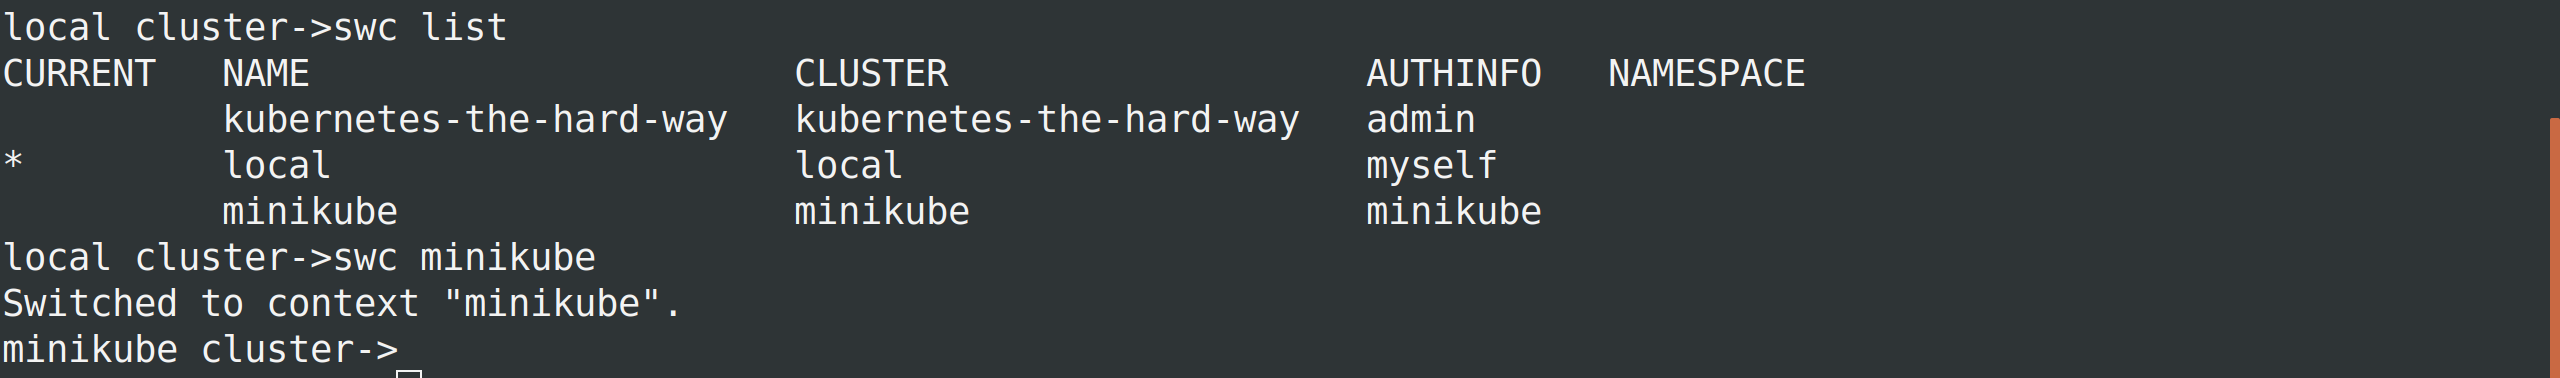
\includegraphics[width=0.9\textwidth]{images/prompt.png}
    \par
	  \caption{Vzhled terminálu\label{fig:prompt}, zdroj: vlastní tvorba}
    \end{centering}
\end{figure}

\subsection{Distribuce Kubernetes node objektů}
    Aplikace umožňuje uživatelům sledovat jednotlivé zdroje a to i servery, které provozují jejich aplikace. V k8s jsou tyto servery označeny jako nody. Na obrázku \ref{fig:nodes-init} je zobrazen seznam dostupných nodů. První je lokální cluster, který reprezentuje virtuální k8s API a obsahuje jeden node s verzí 1.15.0-alpha a dalšími parametry. Druhý cluster minikube obsahuje rovněž jeden node, ovšem s rozdílnými parametry, např. jméno, role nebo verze.\par

\begin{figure}[H]
  \begin{centering}
    
	  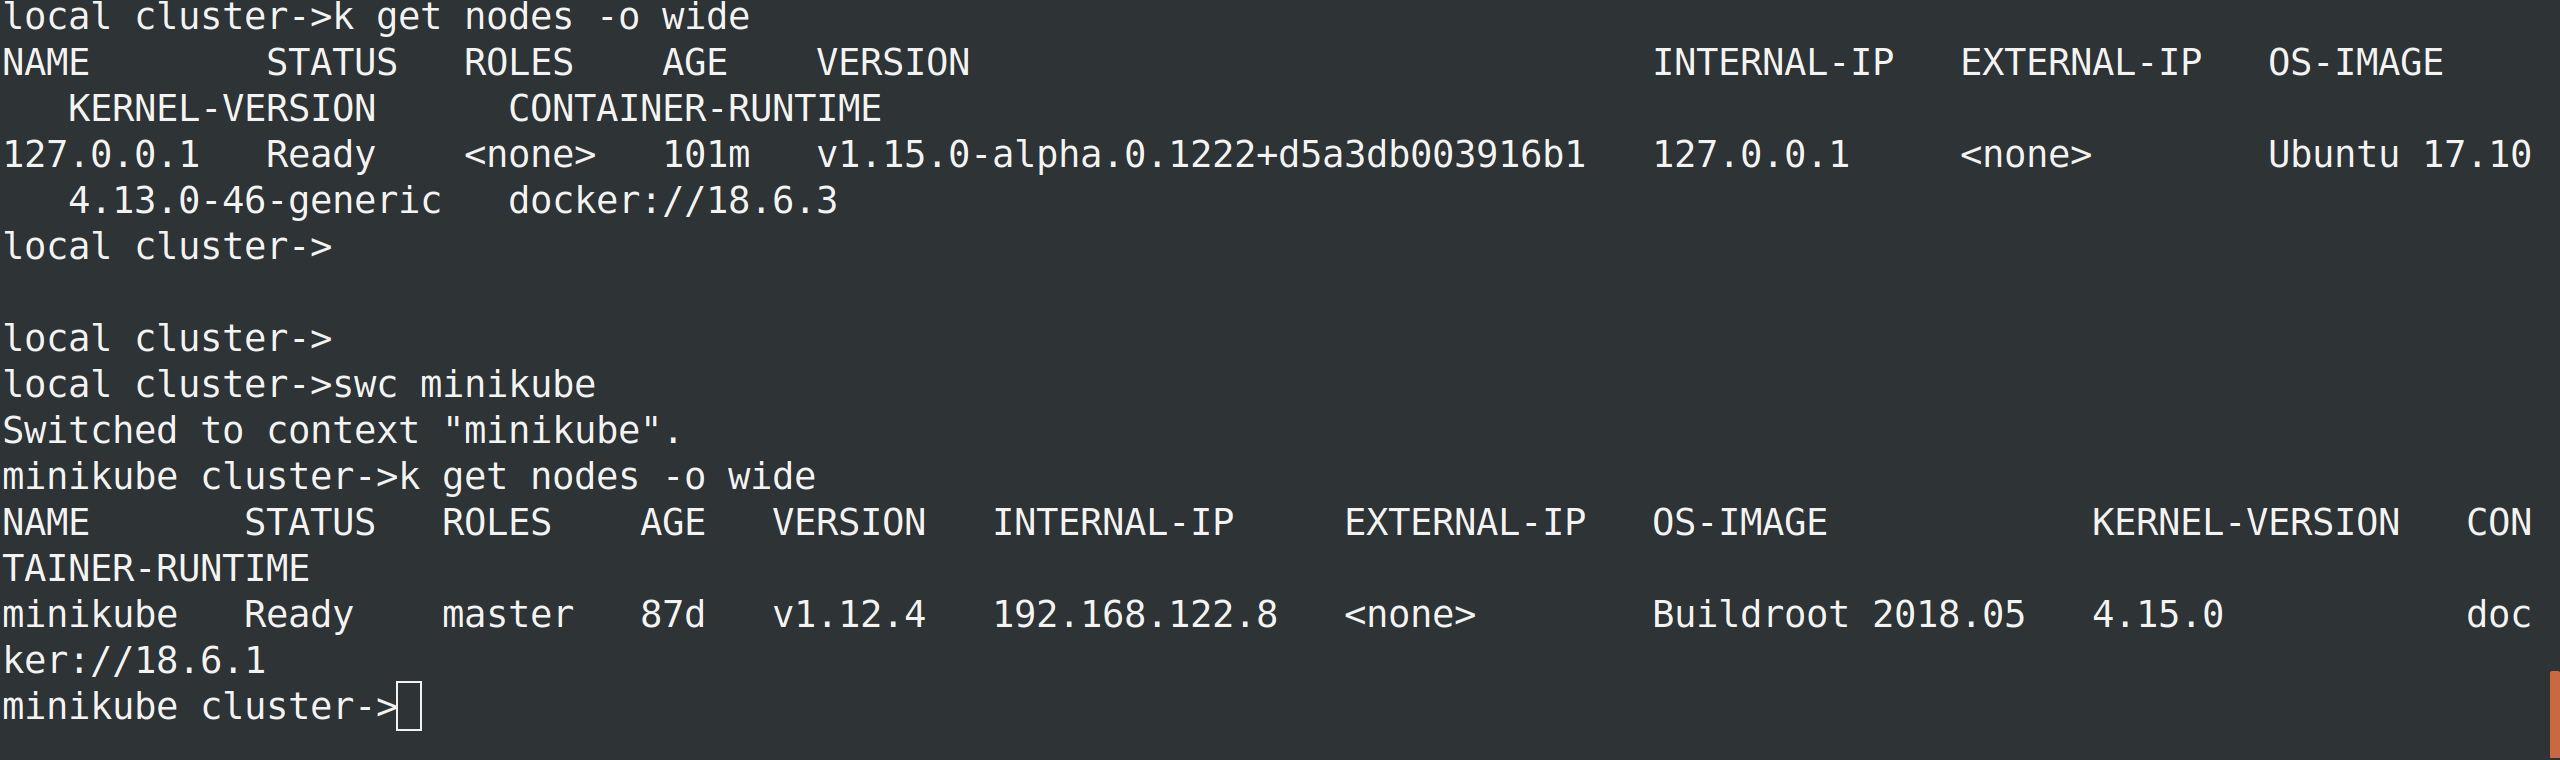
\includegraphics[width=0.9\textwidth]{images/nodes-init.png}
    \par
	  \caption{Seznam nodů v jednotlivých clusterech\label{fig:nodes-init}, zdroj: vlastní tvorba}
    \end{centering}
\end{figure}

    Po spuštění aplikace dojde k inicializace a spuštění managerů. Minikube manager informuje customer manager o dostupných zdrojích. V současné chvíli zde nejsou vytvořeny žádné zdroje. Minikube manager tak oznámí customer manageru informace o nodech, které má zaregistrované. Customer manager tuto událost obdrží a uloží tyto informace do virtuálního k8s API, kde si je uživatelé mohou prohlédnou. Výsledek této akce je uveden na obrázku \ref{fig:nodes-initialized}. Uživateli jsou zobrazeny nody v obou clusterech společně s jejich vlastnostmi.


\begin{figure}[H]
  \begin{centering}
    
	  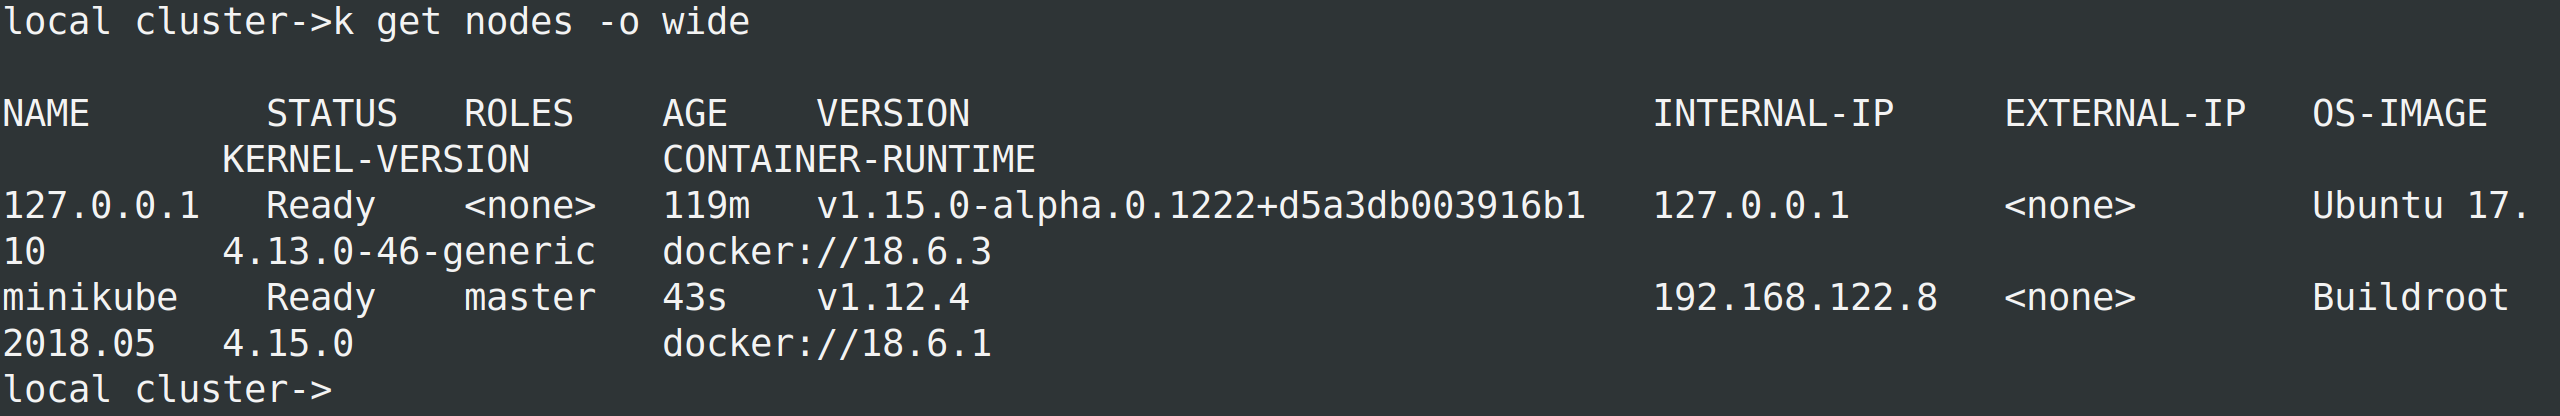
\includegraphics[width=0.9\textwidth]{images/nodes-initialized.png}
    \par
	  \caption{Seznam nodů po spuštění programu\label{fig:nodes-initialized}, zdroj: vlastní tvorba}
    \end{centering}
\end{figure}

\subsection{Distribuce Kubernetes pod objektů}
    Dalším testovaným scénářem je testování distribuce podu z centrálního API do \linebreak Minikube clusteru. Spouštění podů je základní a nezbytná funkce k8s clusterů. Nástroj kubectl umí vytvářet zdroje, které jsou definované s souborech, nazývaných manifesty. Definice podu je uvedena na ukázce kódu \ref{lst:pod}. Definice podu začíná parametrem apiVersion, který specifikuje verzi API, která bude použita pro vytvoření objektu. Parametr Kind uvádí typ objektu, v tomto případě se jedná o pod. Další částí jsou metadata, která připojují další informace o objektu jako jsou jméno nebo id objektu, případně namespace ve kterém má být objekt vytvořen. Posledním blokem jsou spec informace. Zde se nachází definice kontejneru, případně více kontejnerů, který má být v podu spuštěný. Nejdříve je nastaveno, že k8s nemá restartovat kontejner, dále název kontejneru uvnitř podu a definice kontejneru s aplikací. Konkrétně bude spuštěn kontejner BusyBox. Jedná se o malou linuxovou distribuci, která poskytuje základní nástroje pro práci se systémem. Po spuštění kontejneru bude vypsána hláška a dojde k ukončení kontejneru.
\begin{lstlisting}[caption={pod.yml, definice podu},label=lst:pod]
apiVersion: v1
kind: Pod
metadata:
  name: test-pod
  labels:
    app: testapp
spec:
  restartPolicy: Never
  containers:
  - name: test-container
    image: busybox
    command: ['sh', '-c', 'echo Hello world !']
\end{lstlisting}
			  Proces vytvoření zdroje pod je uvedena na obrazku \ref{fig:pod}. Po aplikovaní manifest souboru je spuštěn proces vytvoření zdroje. Customer manager zjistí vytvoření zdroje pod a vytvoří událost s odpovídajícími parametry, kterou odešle do minikube manageu. Ten vytvoří pod v minikube clusteru a o jeho stavu informuje customer manager. Pod se nejdříve nachází ve stavu Pending, během něhož je určeno na kterém nodu bude spuštěn a také dochází ke stažení potřebného kontejner image. Poté je kontejner ve stavu Running, neboli vykonává zadaný kód, výpis hlášky. Po úspěšném dokončení výpisu přechází kontejner do stavu Completed. Stejný výstup vypíše i minikube cluster. Stav podu je shodný v obou clusterech.
			  Z minikube clusteru je možné vypsat průběh programu. Zde je vidět, že program vypsal hlášku “Hello world !”. Posledním krokem je odstranění podu. Zde bylo potřebné upravit kod aplikace, Aplikace totiž sleduje zdroje v určeném namespacu a aplikuje všechny informace o těchto zdrojích do minikube clusteru v případě customer managera. Na druhé straně minikube manager aplikuje všechny změny z minikube k8s clusteru do centrálního API s využitím customer managera. Při tomto nastavení docházelo k zacyklení aplikace. Zdroj byl sice smazán v centrálním API ale než tato informace doputovala do minikube clusteru, minikube manager oznámil centrálnímu API informace o běžícím podu. Jako řešení je použit postup v customer manageru, který ověří příchozí události z minikube managera a dovolí vytvořit pouze objekt Node. Vytvoření je reprezentováno jako parametr type s hodnotou Added struktury Event, která reprezentuje událost. 
			   
\begin{figure}[H]
  \begin{centering}
    
	  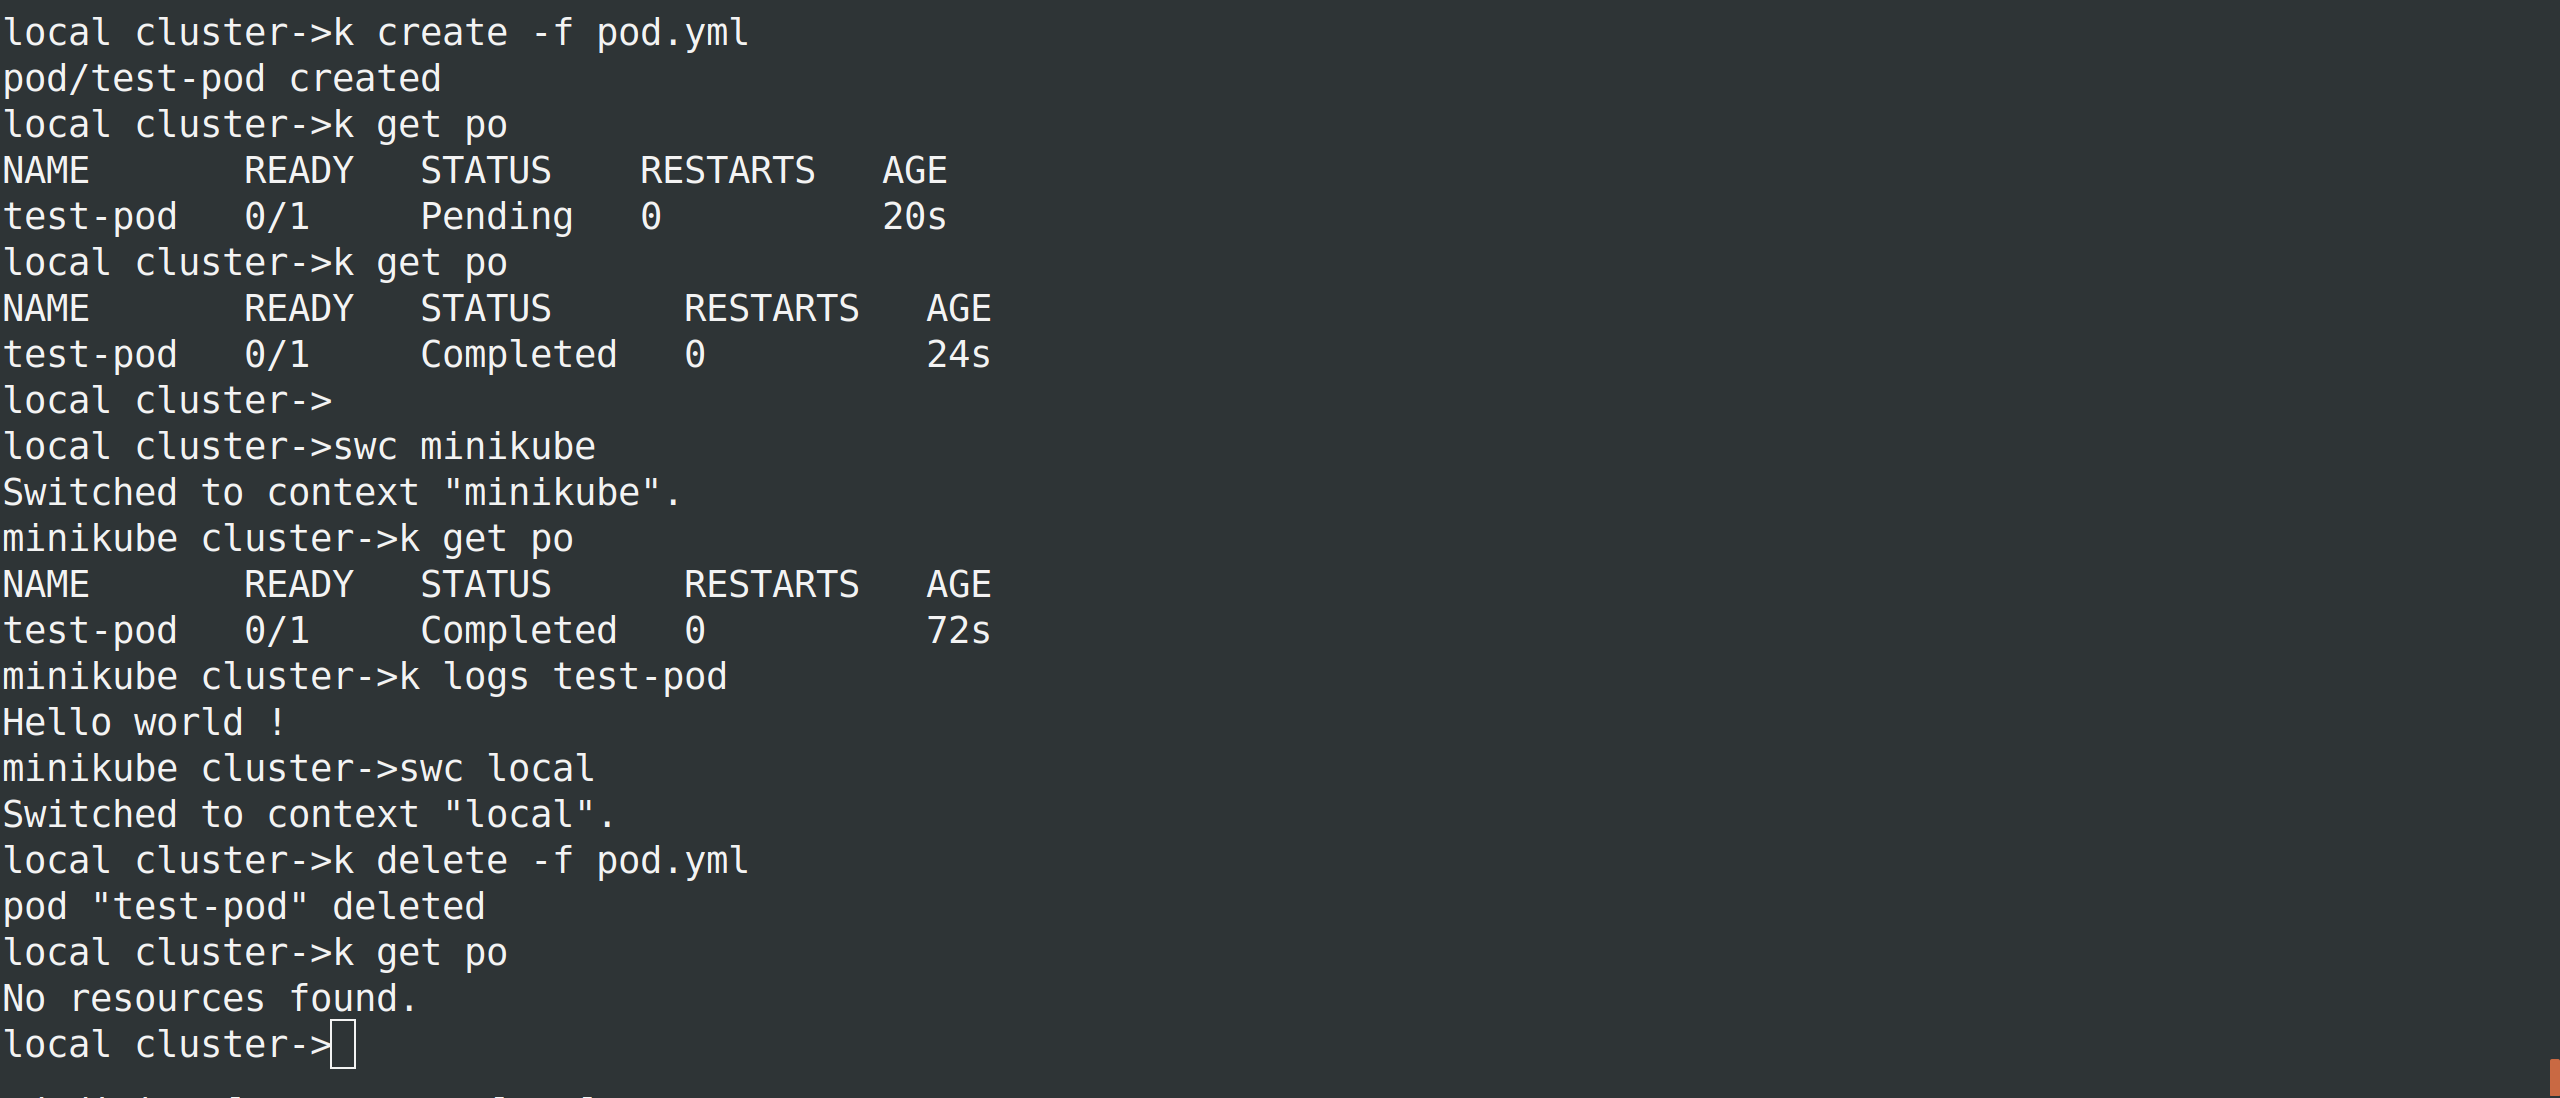
\includegraphics[width=0.9\textwidth]{images/pod.png}
    \par
	  \caption{Práce s pody\label{fig:pod}, zdroj: vlastní tvorba}
    \end{centering}
\end{figure}

\subsection{Distribuce Kubernetes deployment objektů}
Deploymenty řídí bezstavové, stateless, aplikace běžící v clusteru. Deployment umí udržovat potřebný počet kontejnerů, zvyšovat nebo snižovat počet kontejnerů, provádět přechod na novější verzi aplikace, případně vrátit původní verzi aplikace v případě, že nová verze obsahuje chyby. Definice deploymentu je uvedena na ukázce kódu \ref{lst:deployment}. V části spec je specifikován počet kontejnerů, neboli počet instancí aplikace. Další důležitou částí je selector, podle kterého jsou vybrány spravované kontejnery. Diky selectoru například udržuje deployment počet kontejnerů, pokud je počet kontejnerů s požadovaným labelem menší než je definováno, jsou vytvořeny nové kontejnery. V bloku template je definovaný kontejner a také jeho label a port na kterém aplikace poslouchá.
\begin{lstlisting}[caption={deployment.yml, definice deploymentu},label=lst:deployment]
apiVersion: apps/v1
kind: Deployment
metadata:
  name: diplomka-nginx-deployment
  labels:
  app: dnd
spec:
  replicas: 2
  selector:
    matchLabels:
      app: dnd
  template:
    metadata:
      labels:
      app: dnd
    spec:
      containers:
      - name: diplomka-nginx
        image: casek14/diplomka-nginx:v1
        ports:
        - containerPort: 80
\end{lstlisting}
													     Aplikace, která bude spuštěna pomocí výše definovaného deploymentu je jednoduchý webový server Nginx, který bude zobrazovat statickou stránku. Aplikace bude přijímat požadavky na portu 80. Tento port není přístupný pro uživatele. Pro přístup uživatelů bude ještě vytvořen zdroj Service, který umožní přístup uživatelů k vytvořené aplikaci. Service je opět definovaná pomocí manifest souboru \ref{lst:service}. Důležitá část definice servicy je selector, který říká na které kontejnery má service směřovat požadavky. Typ service NodePort znamená, že na serveru s kontejnerem aplikace je připraven port pro přístup ke kontejnerům deploymentu. Service umí také Load-Balancing mezi spuštěnými kontejnery. 
\begin{lstlisting}[caption={service.yml, definice service},label=lst:service]
apiVersion: v1
kind: Service
metadata:
  name: diplomka-nginx-service
spec:
  selector:
    app: dnd
  type: NodePort
  ports:
  - protocol: TCP
    port: 8080
    targetPort: 80
\end{lstlisting}

Na obrázku \ref{fig:create-deployment} je vidět postup nasazení deploymentu a service, která aplikaci zpřístupní uživatelům. K8s nasazení aplikace zabere určitý čas. Po přibližně 15 vteřinách je deployment ve fázi vytváření kontejnerů, což znamená stahování kontejneru. Proces spuštění kontejnerů zabral přibližně dvě a půl minuty. V produkčním prostředí s rychlým internetem by takový proces zabral okolo dvaceti vteřin. 


\begin{figure}[H]
  \begin{centering}
    
	  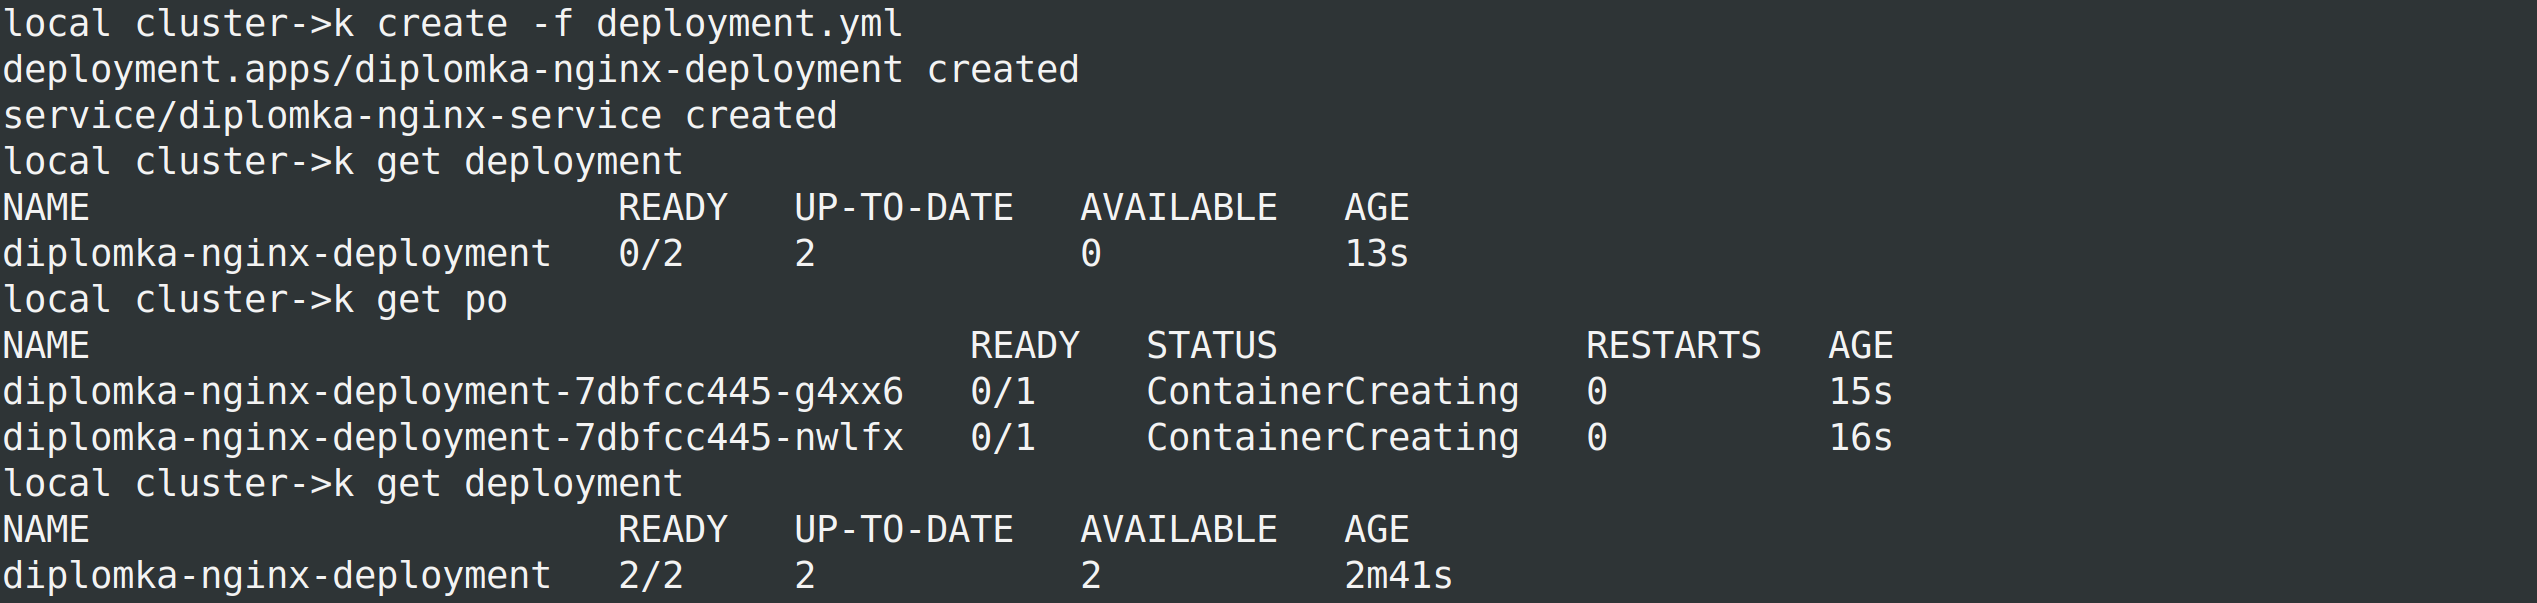
\includegraphics[width=0.9\textwidth]{images/create-deployment.png}
    \par
	  \caption{Vytvoření deploymentu\label{fig:create-deployment}, zdroj: vlastní tvorba}
    \end{centering}
\end{figure}

Výsledná aplikace je zobrazena na obrázku \ref{fig:v1}. Aplikace je dostupná na portu, který minikube cluster alokoval. V definici deploymentu byla specifikována verze 1, která koresponduje s hlavním titulkem na obrázku \ref{fig:v1}.

\begin{figure}[H]
  \begin{centering}
    
	  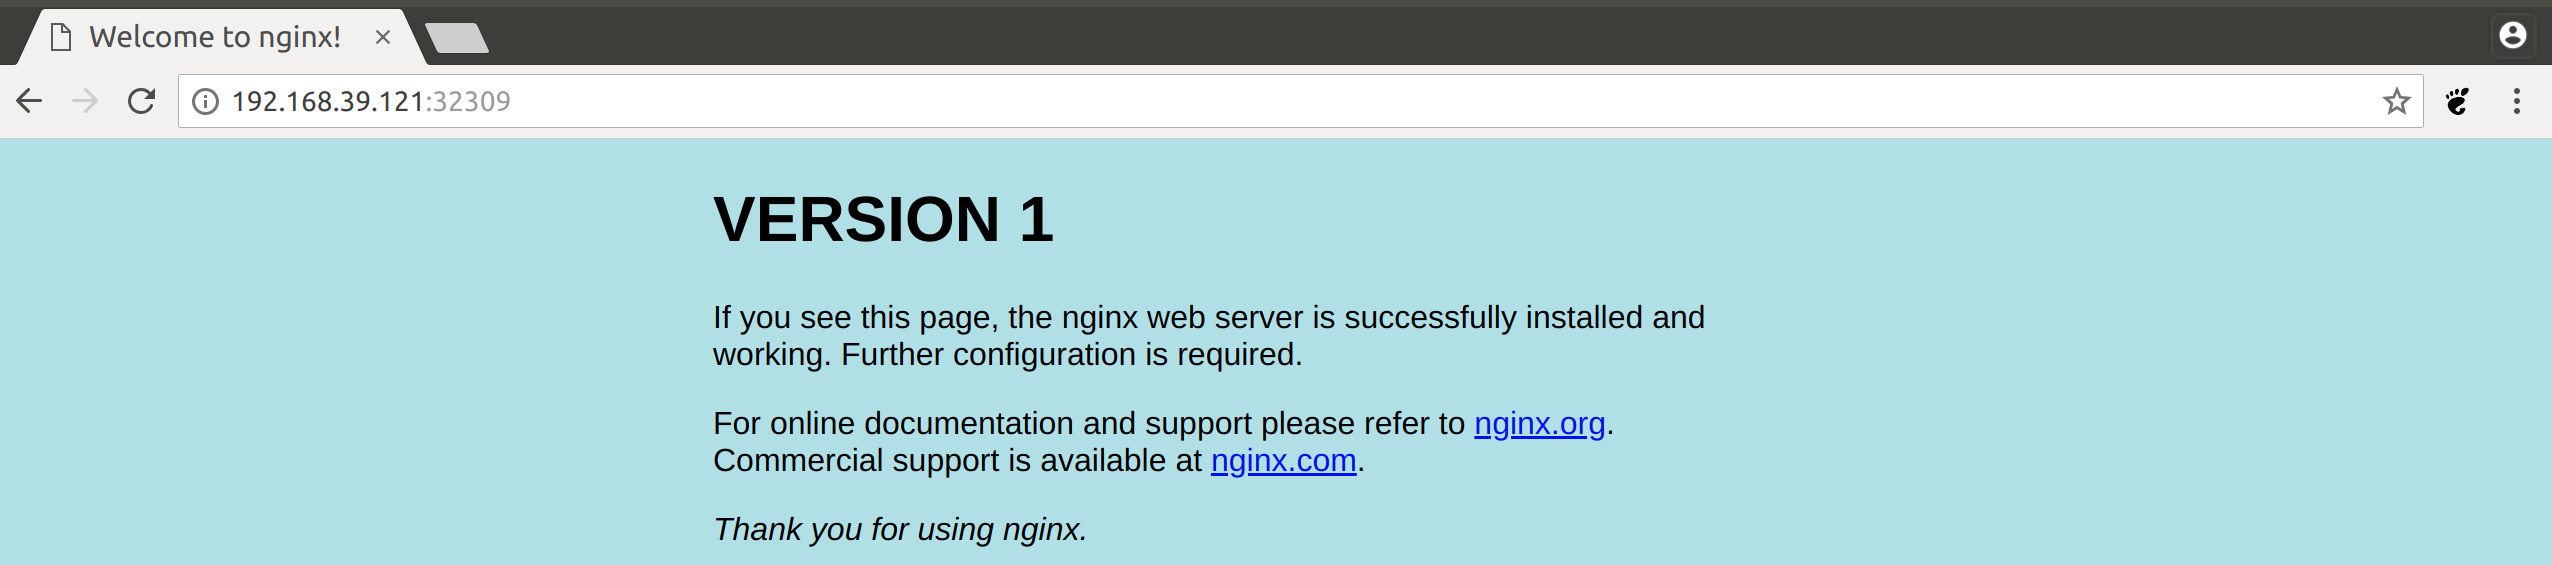
\includegraphics[width=0.9\textwidth]{images/v1.png}
    \par
	  \caption{Vzhled aplikace verze 1\label{fig:v1}, zdroj: vlastní tvorba}
    \end{centering}
\end{figure}

Jedním z rysů a výhod cloud native přístupu je doručování nových verzí aplikace. Cloud native aplikace nejsou statické co se týče nových funkcí a vylepšení. K8s dovoluje snadné nahrazení stávající verze novou verzí. V následujícím příkladu bude aplikace s verzí 1 nahrazena verzí aplikace 2. Postup přepnutí verze aplikace na verzi 2 je uveden na obrázku \ref{fig:update-deployment}. Na prvním řádku je zobrazena verze aplikace před upgradem. Na druhém řádku je pomocí příkazu edit uvedena změněna verze v definici deploymentu, která je následně zobrazena. V tomto okamžiku již k8s provádí vypnutí kontejnerů verze 1 a začíná s postupným startováním kontejnerů s verzí 2. Aplikace s novou verzí je zobrazena obrázku \ref{fig:v2}, aplikace je dostupná na stejné adrese a portu.

\begin{figure}[H]
  \begin{centering}
    
	  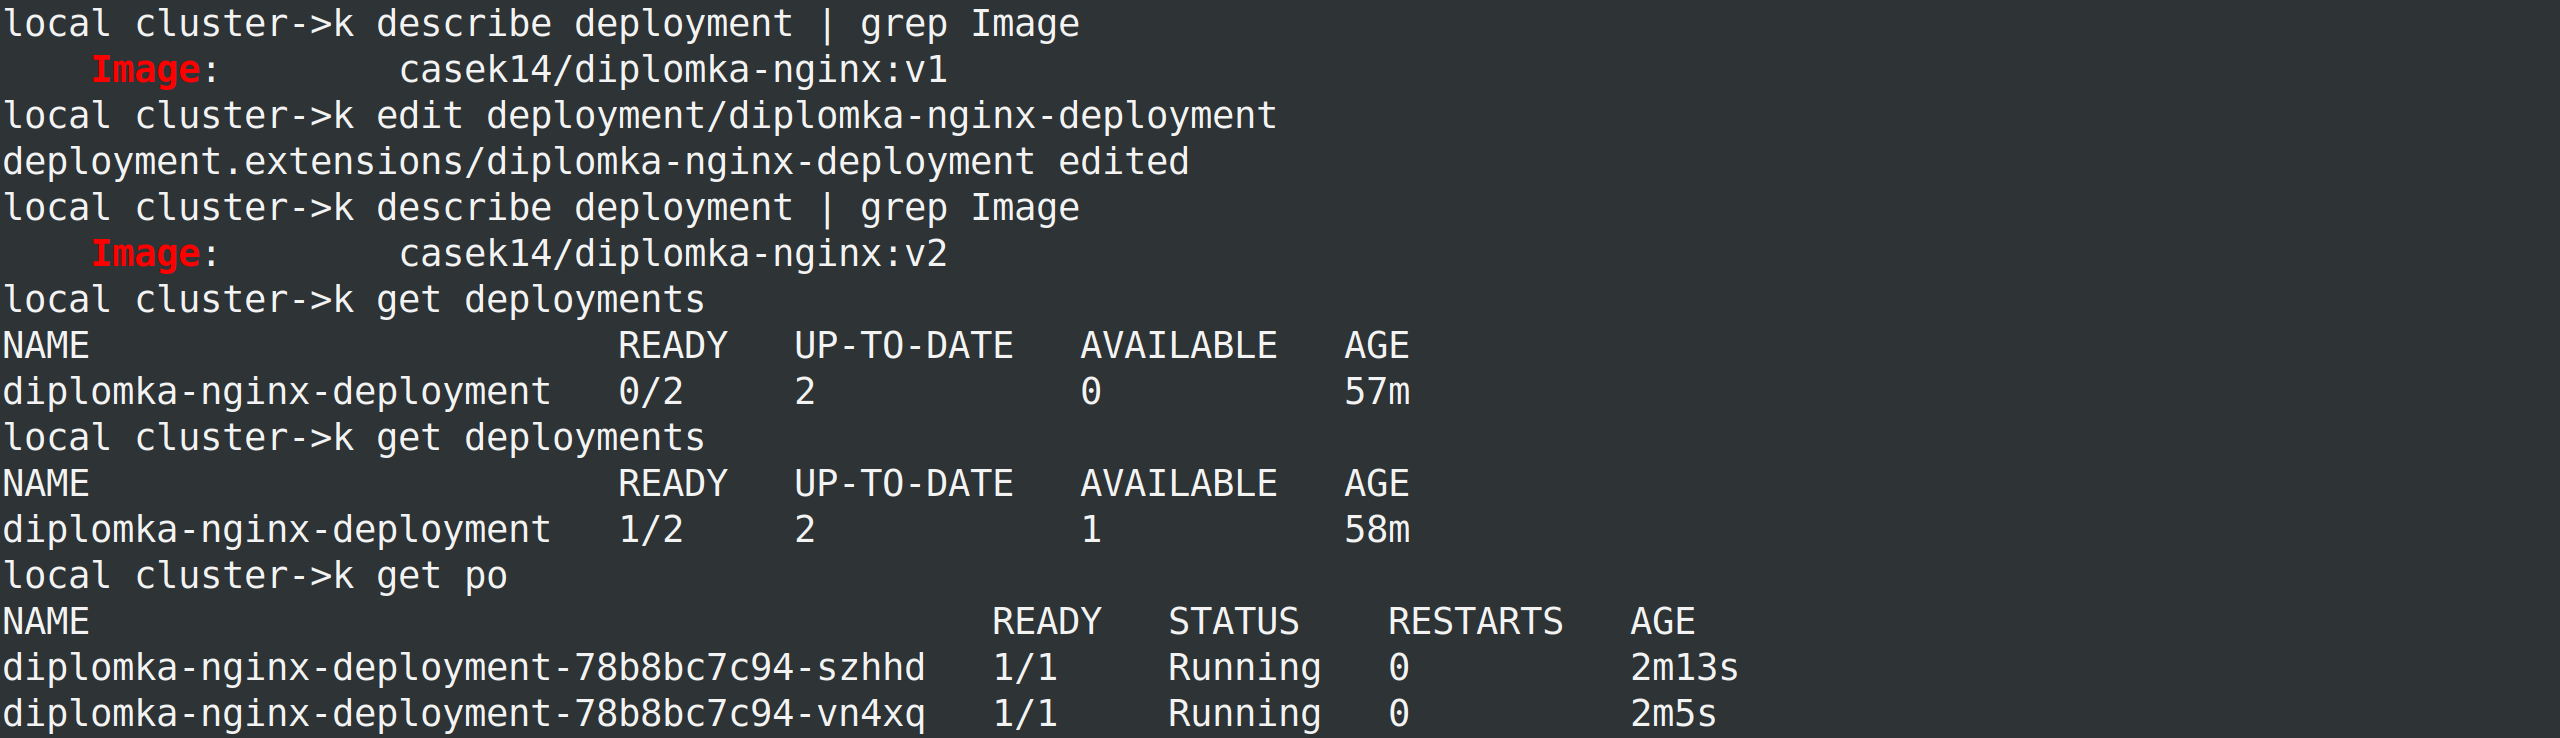
\includegraphics[width=0.9\textwidth]{images/deployment-update.png}
    \par
	  \caption{Úprava deploymentu\label{fig:update-deployment}, zdroj: vlastní tvorba}
    \end{centering}
\end{figure}

\begin{figure}[H]
  \begin{centering}
    
	  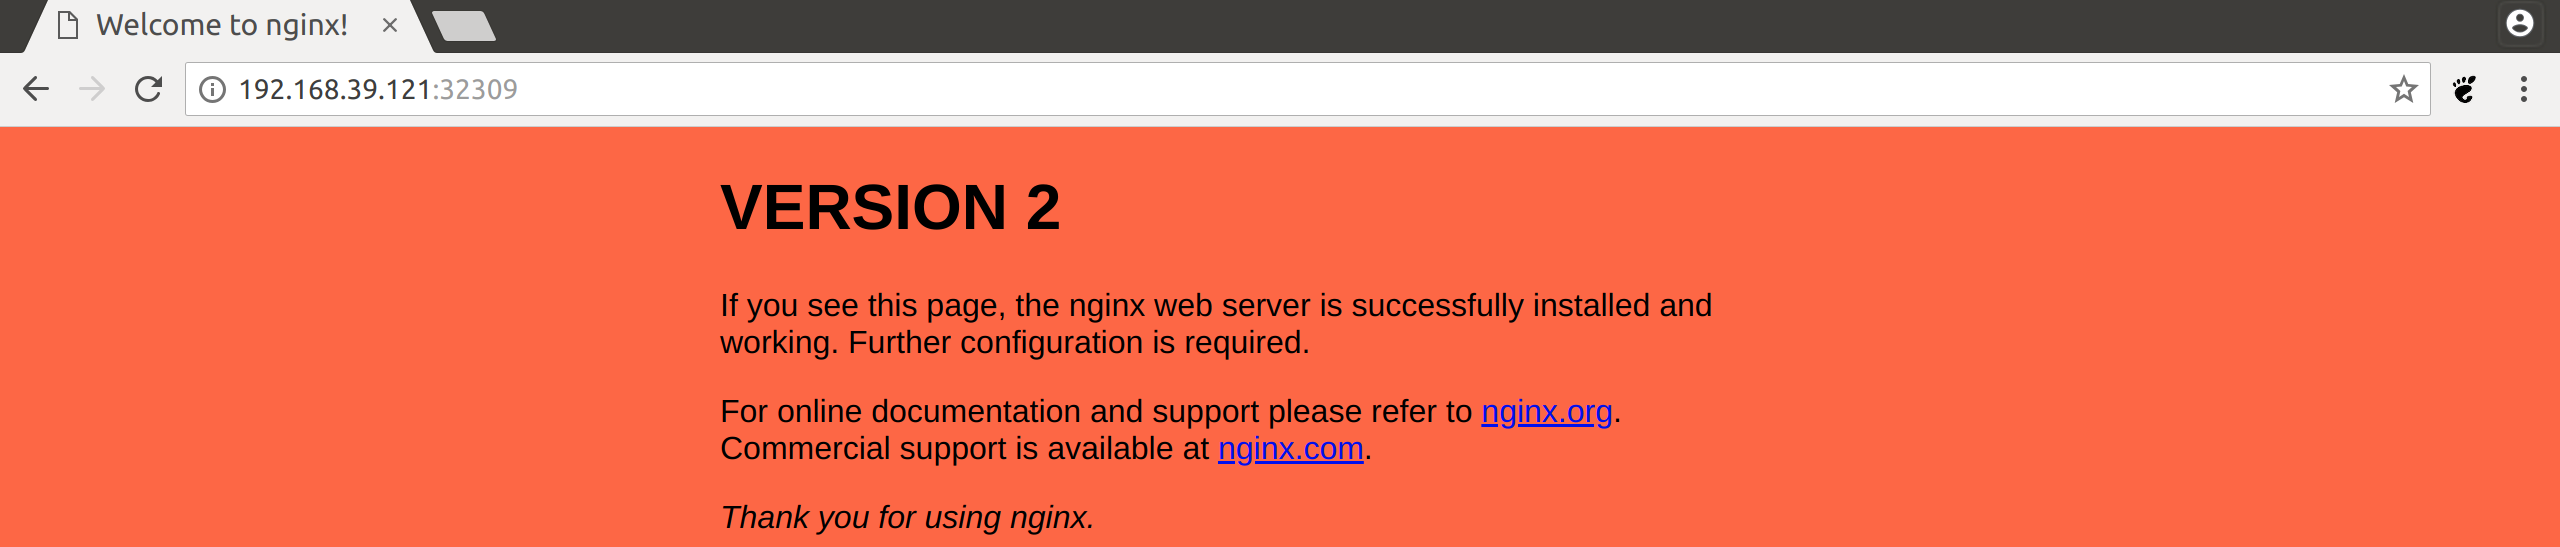
\includegraphics[width=0.9\textwidth]{images/v2.png}
    \par
	  \caption{Vzhled apliakce verze 2\label{fig:v2}, zdroj: vlastní tvorba}
    \end{centering}
\end{figure}
Deployment může být použitý také pro vrácení chybné verze aplikace. Tato technika je užitečná v okamžiku, že se do produkčního prostředí dostane verze aplikace, která nefunguje nebo obsahuje bug. Při testování této funkce, které je zobrazeno na obrázku \ref{fig:deployment-rollout}, je nejdříve vytvořen deployment s aplikací verze 1. Následně byla verze aplikace změněna na verzi 2, tato akce byla uložena pomocí volby “--record”. K8s si tuto akci uloží, aby bylo možné se vrátit o krok zpět. Následně je změněna verze aplikace na v3. Třetí verze aplikace je zobrazena na obrázku \ref{fig:v3}. Po nasazení třetí verze je ovšem zjištěno, že barva pozadí aplikace neodpovídá zadání. Zřejmě došlo k pochybení programátora, a barva pozadí neodpovídá barvám, které společnost využívá. Proto je rozhodnuto vrátit aplikaci do verze 2. K tomuto účelu byla využita funkce “rollout”, která vrátí verzi aplikace o jeden krok zpět na požadovanou verzi 2.

\begin{figure}[H]
  \begin{centering}
    
	  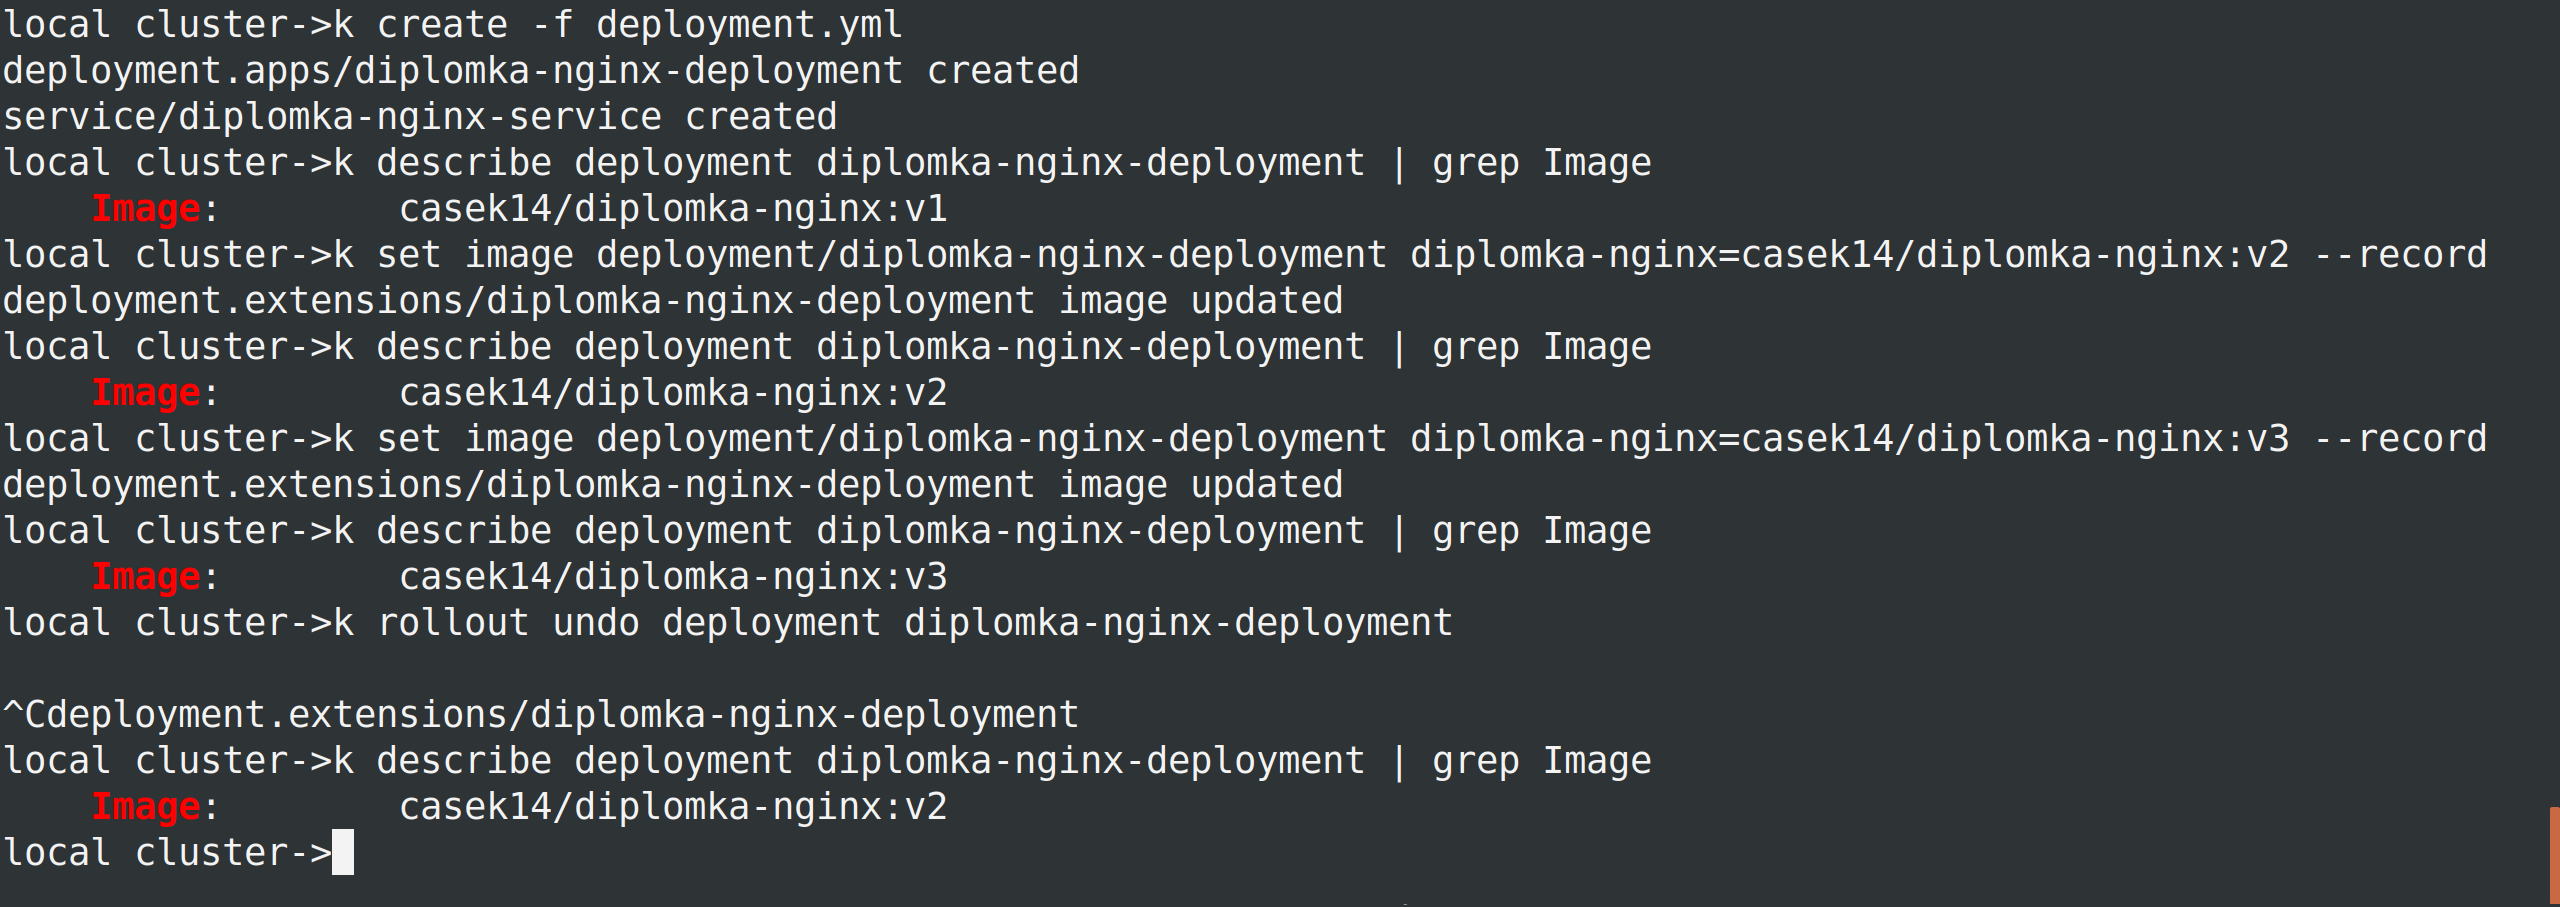
\includegraphics[width=0.9\textwidth]{images/rollout.png}
    \par
	  \caption{Vrácení verze aplikace pomocí rollout funkce\label{fig:deployment-rollout}, zdroj: vlastní tvorba}
    \end{centering}
\end{figure}

\begin{figure}[H]
  \begin{centering}
    
	  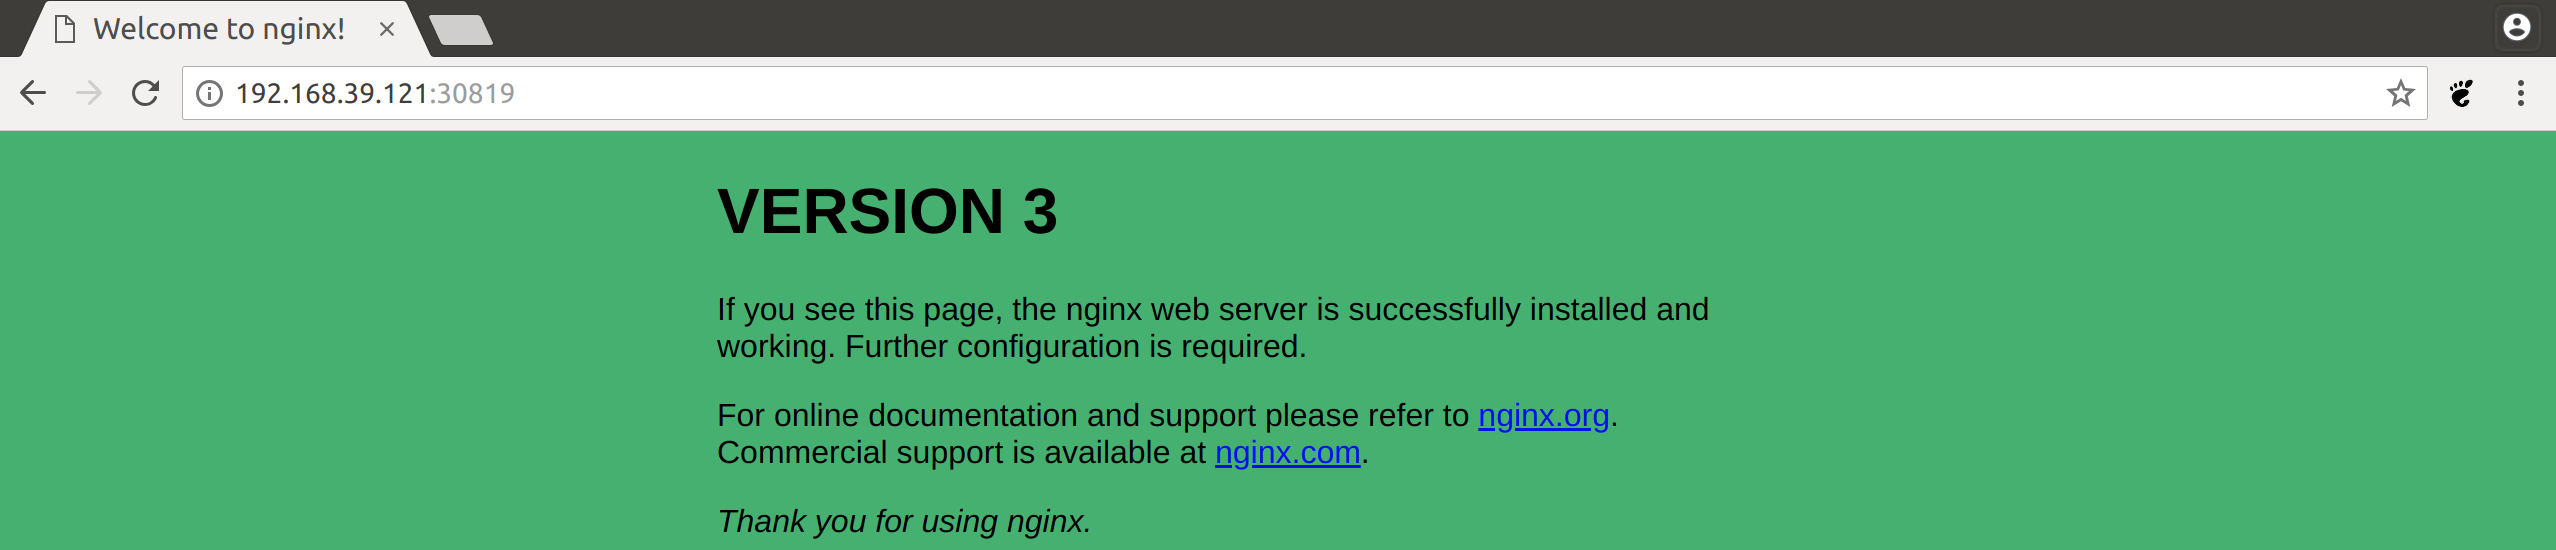
\includegraphics[width=0.9\textwidth]{images/v3.png}
    \par
	  \caption{Vzhled aplikace verze 3\label{fig:v3}, zdroj: vlastní tvorba}
    \end{centering}
\end{figure}

Jedním z testovaných aspektů je i škálování aplikací. Pokud současný počet instancí aplikace nestíhá obsloužit všechny zákazníky je potřeba zvýšit jejich počet. K8s opět nabízí pro tento účel nástroje, které dovolují operátorům jednoduše zvýšit počet instancí. Service se postará o rozložení zátěže mezi všechny nové pody. Na obrázku \ref{fig:scale1} je vytvořen deployment, který se skládá ze dvou podů a také service směřující požadavky na tyto pody. Každý pod na portu 80 odpovídá na požadavky se svým jménem kontejneru. Zdrojový kód této aplikace je uveden v příloze \hyperref[app:hostname]{A}. Dále je spuštěn skript, který desetkrát pošle požadavek na service a vypíše odpověď. Z obrázku je patrné, že požadavky vyřizují pouze dva pody.

\begin{figure}[H]
  \begin{centering}
    
	  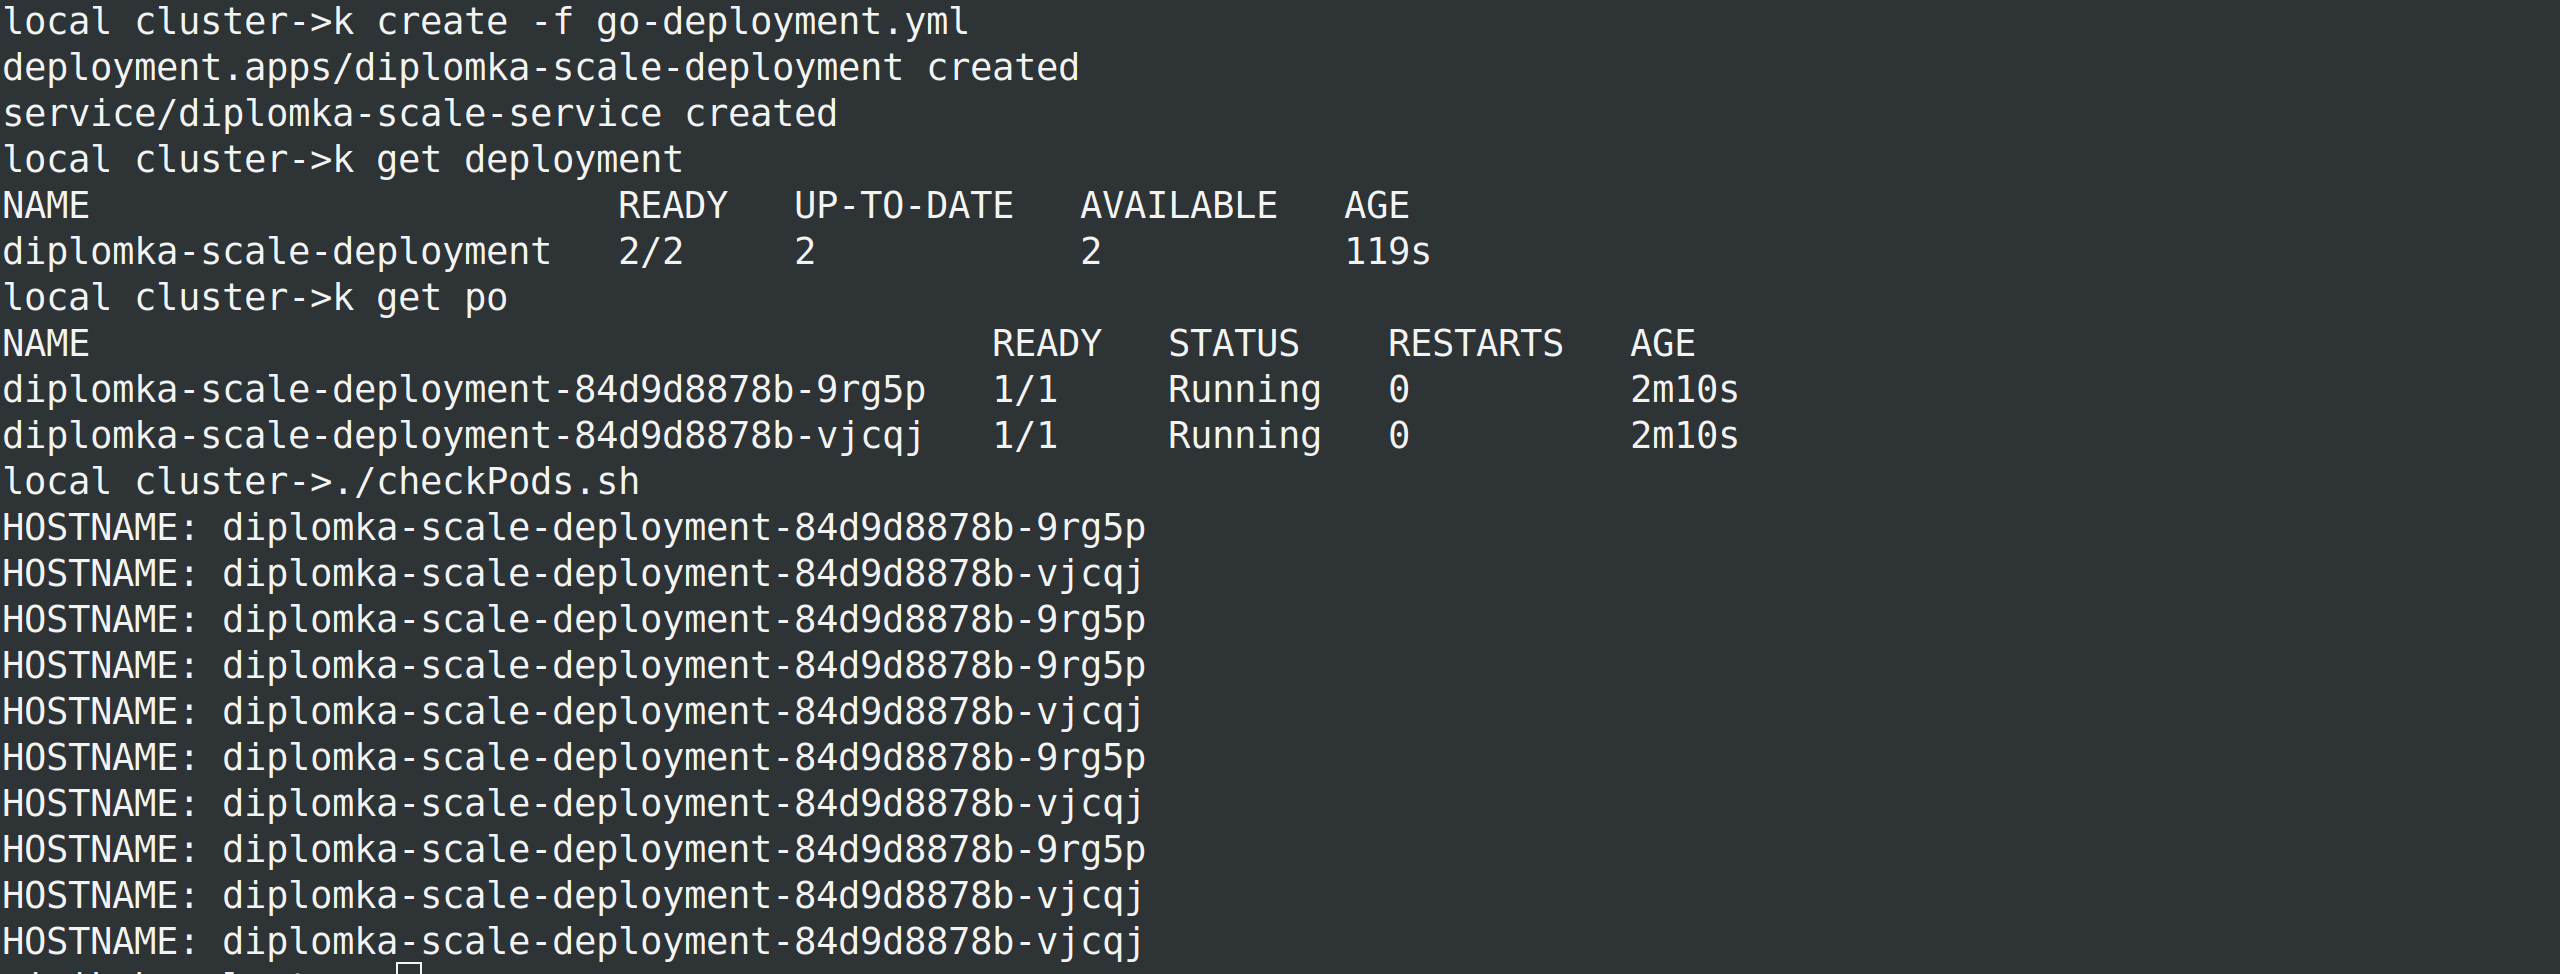
\includegraphics[width=0.9\textwidth]{images/scale1.png}
    \par
	  \caption{Test deploymentu se 2 pody\label{fig:scale1}, zdroj: vlastní tvorba}
    \end{centering}
\end{figure}

V dalším kroku je počet podů, které budou vyřizovat požadavky uživatelů zvýšen na deset \ref{fig:scale2}. K8s ihned začne startovat nové kontejnery tak, aby bylo dosaženo \linebreak požadovaného počtu deseti instancí aplikace. V přehledu podů je vidět, že dva původní pody zůstaly a k nim byly vytvořeny další pody. Patrné je to podle parametru “AGE” neboli stáří kontejneru.

\begin{figure}[H]
  \begin{centering}
    
	  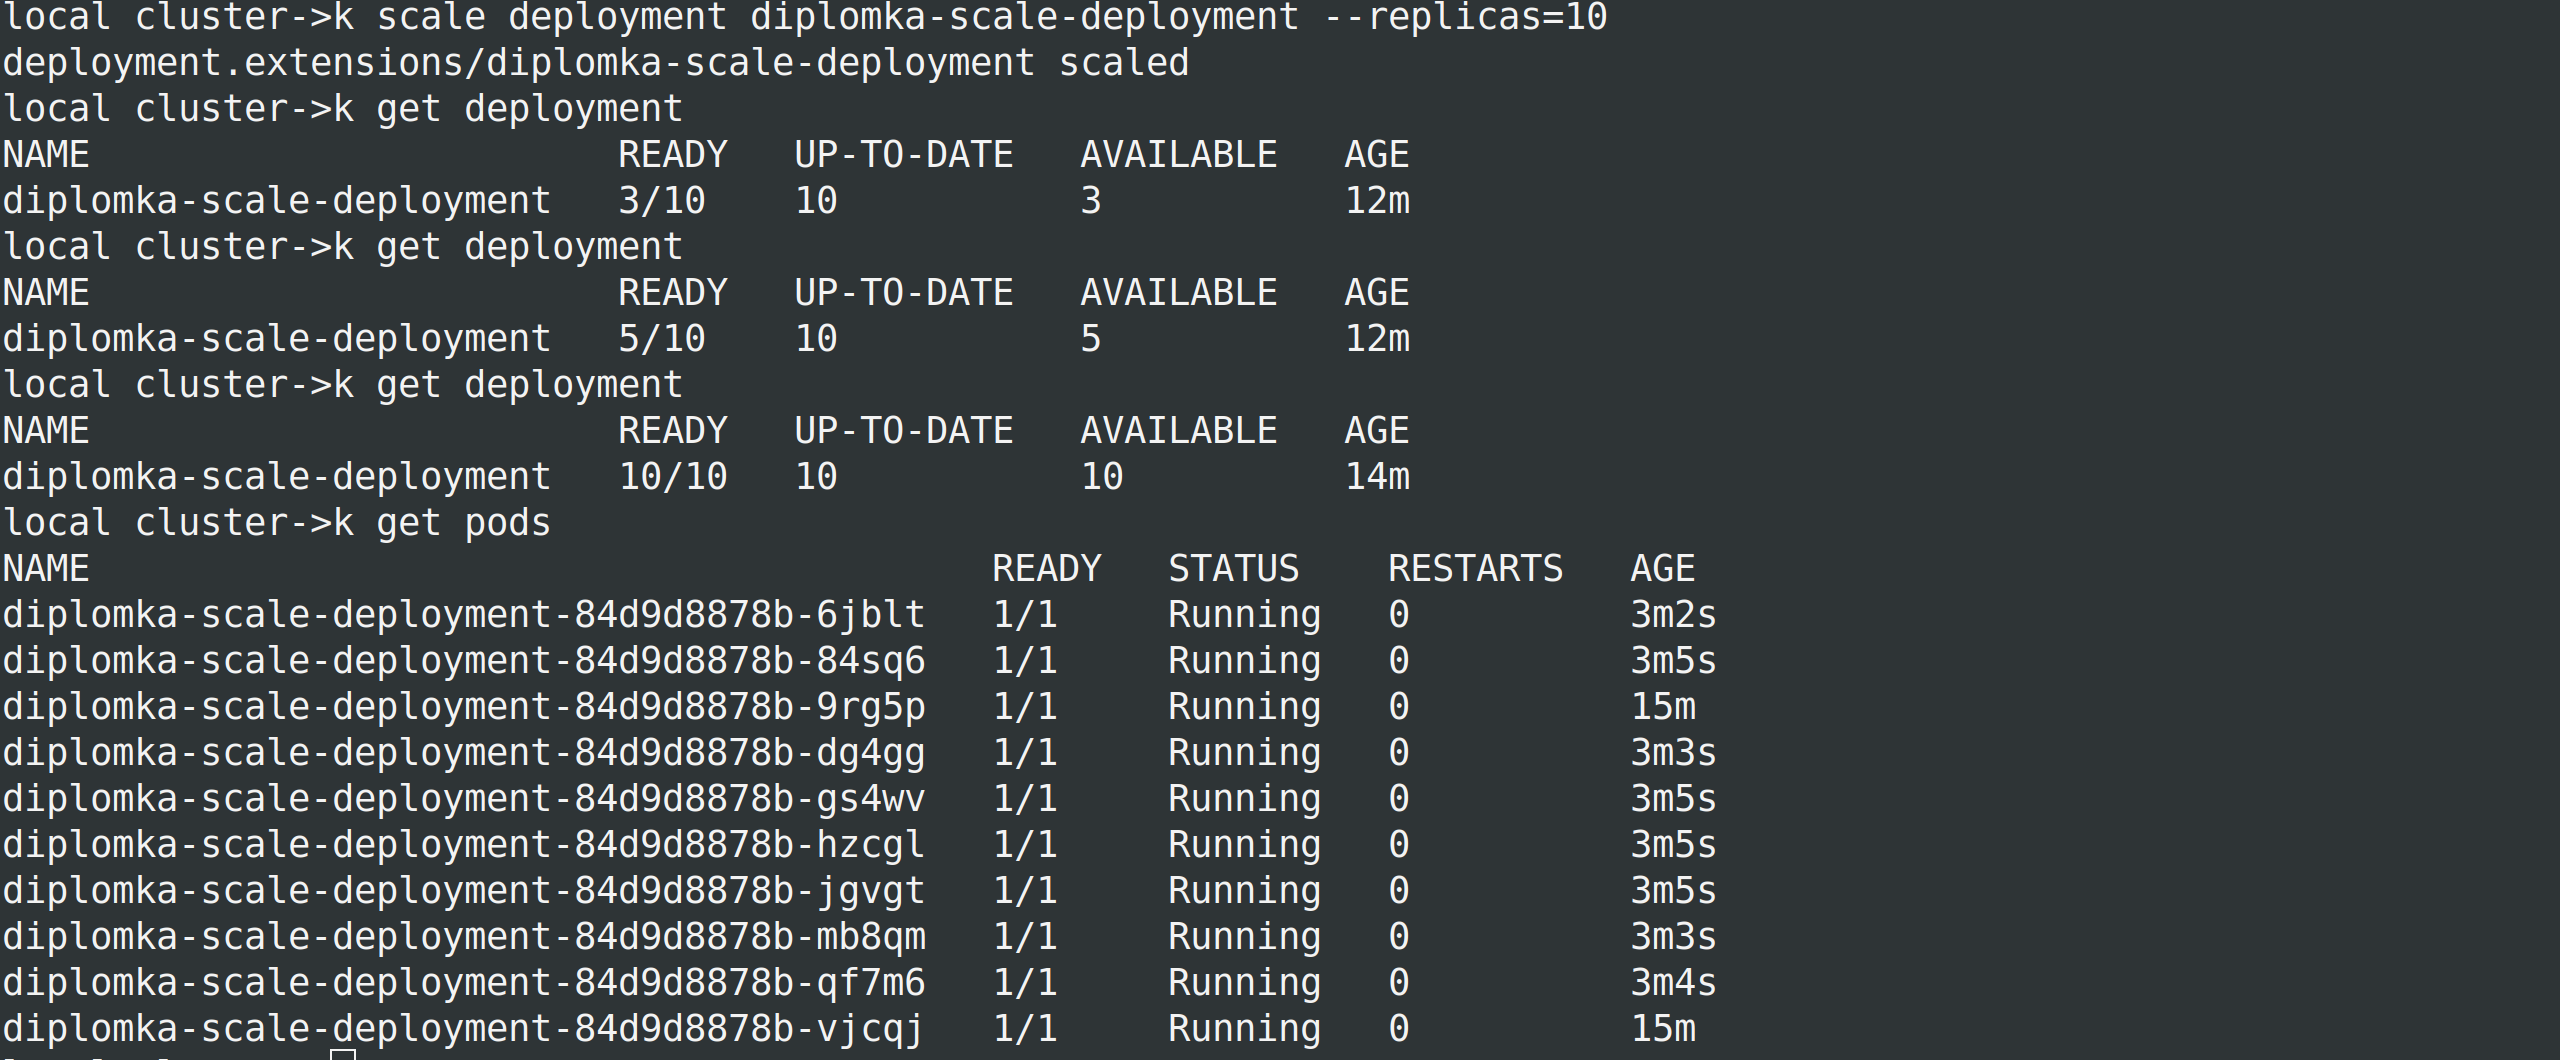
\includegraphics[width=0.9\textwidth]{images/scale2.png}
    \par
	  \caption{Škálování deploymentu ze 2 na 10 podů\label{fig:scale2}, zdroj: vlastní tvorba}
    \end{centering}
\end{figure}

Servica, která se stará o rozdělení zátěže, směřuje požadavky i na nově vytvořené pody, které vybírá podle labelu app=golang. Na obrázku \ref{fig:scale3} je zobrazen výstup ze skriptu, požadavky směřují pokaždé na jeden z deseti podů, které obsahují aplikaci.

\begin{figure}[H]
  \begin{centering}
    
	  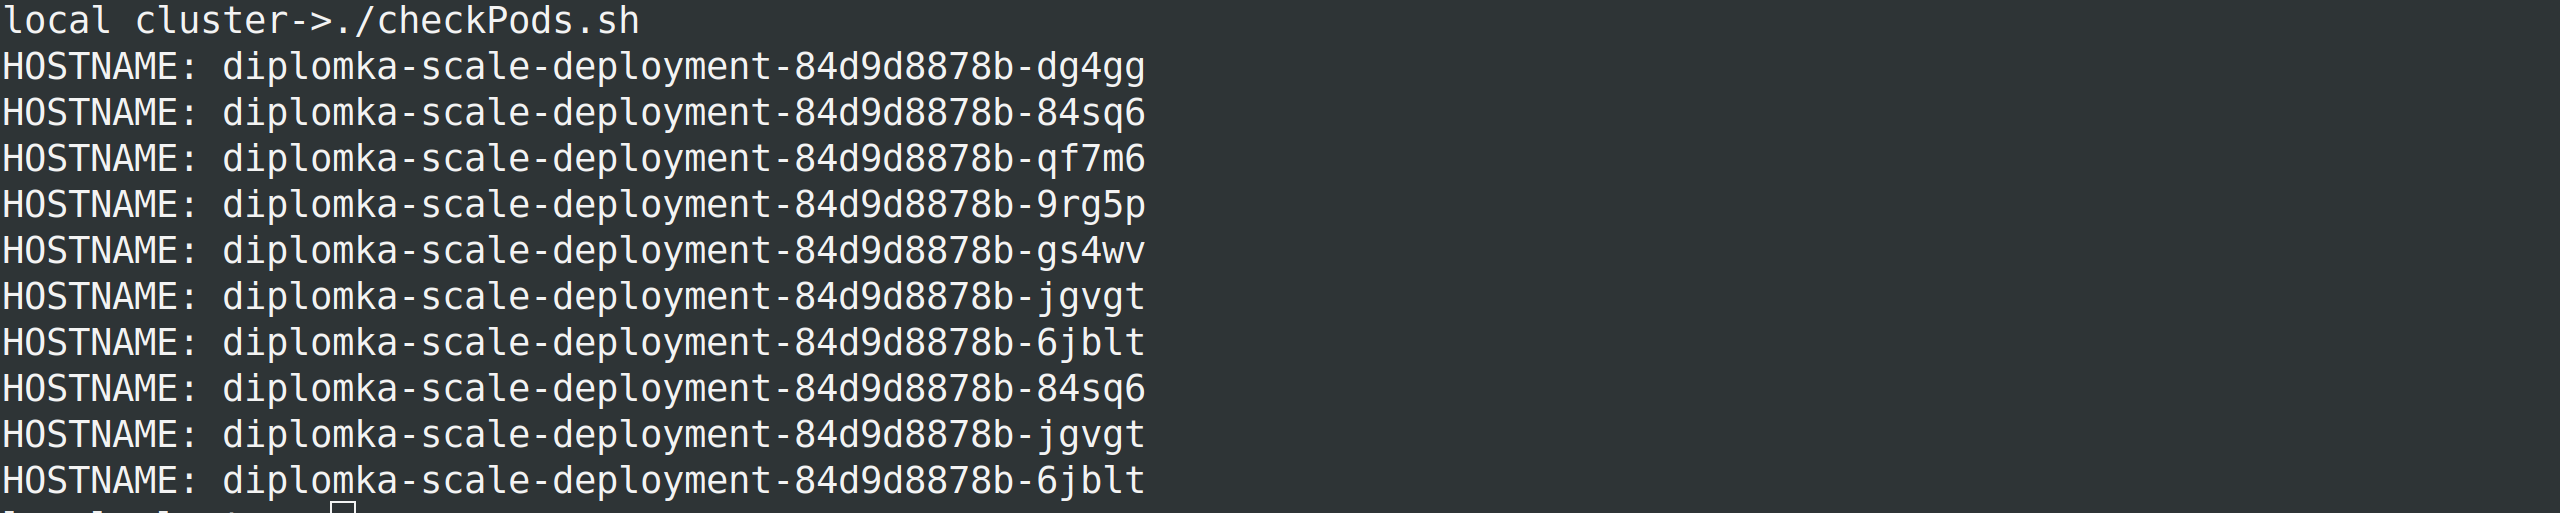
\includegraphics[width=0.9\textwidth]{images/scale3.png}
    \par
	  \caption{Test dostupnosti deploymentu s 10 pody\label{fig:scale3},  zdroj: vlastní tvorba}
    \end{centering}
\end{figure}

\subsection{Distribuce Kubernetes statefulset objektů}
Kubernetes umožňuje běh stateful aplikací, které uchovávají a spravují data. Příkladem stateful aplikací jsou databáze. Databáze potřebují uložiště pro data, které vydrží restart kontejnerů. Tato funkcionalita je v k8s reprezentována pomocí zdroje statefulset. Statefulset je obdobou deploymentu, ale pro stateful aplikace. Statefulset řídí počet replik, jejíž pody jsou vytvářeny jeden po druhém, mají definované pořadí a přiřazené stejné uložiště. Pokud statefulset obsahuje tři repliky, jako první se vytvoří replika jedna a až po jejím úspěšném vytvoření a spuštění se začne spouštět druhá replika a poté následuje třetí replika. Uložiště je do podu připojeno jako volume. Ovšem statefulset po restartování kontejneru tento volume nesmaže a tak nedojde ke ztrátě dat. Pro vytvoření volumu jsou použity tři k8s zdroje storageclass, persistenvolume (PV) a persistentvolumeclaim (PV). Storageclass představuje reprezentaci uložiště, kterou k8s cluster nabízí a obsahuje například parametr provisioner, který specifikuje jaký typ uložiště bude použitý. Může být použit NFS, CEPH a spoustu dalších. Příklad definice storage class je uveden v ukázce kódu \ref{lst:storageclass}. PV abstrahuje implementační detaily jednotlivých typů uložišť a je spravováno administrátorem k8s clusteru. PVC je požadavek uživatele pro přidělení uložiště pro určitý pod. PVC je alokováno z PV. 

\begin{lstlisting}[caption={StorageClass definice pro minikube cluster},label=lst:storageclass]
kind: StorageClass
apiVersion: storage.k8s.io/v1
metadata:
  name: minikube-class
  provisioner: k8s.io/minikube-hostpath
  reclaimPolicy: Retain
\end{lstlisting}

\par
      Pro otestování distribuce stateful aplikací je použita jednoduchá aplikace, která po svém spuštění vytvoří ve specifickém adresáři soubor, jehož jméno je složeno z hostnamu daného kontejneru a časového údaje, kdy byl vytvořen. Aplikace následně po vytvoření souboru zpřístupní tento adresář se souborem na portu 3000. Zdrojový kód aplikace je uveden v příloze \hyperref[app:servefiles]{B}. Pro spuštění této aplikace je použitý manifest soubor uvedený v příloze \hyperref[app:statefulset]{C}. Definice statefulsetu začíná definicí názvu této aplikace, následuje specifikace selektoru, tedy jaké pody patří k tomuto statefulsetu. Definice kontejneru a portu na kterém aplikace zpracovává požadavky je známá z předchozích příkladů. Definice “volumeMounts” reprezentuje trvalé uložiště, které bude připojené ke kontejneru a do něhož bude aplikace ukládat zmíněné soubory. Definice samotného uložiště je uvedena pod částí “volumeClaimTemplates”, která říká jaké uložiště bude použito. Parametr “storageClassName” se shoduje s názvem v definici pro strorageclass \ref{lst:storageclass}. Velikost uložiště, které bude připojené k podu připojené má velikost 1GB. Poslední částí definice statefulsetu je definice systémové proměné “DIRECTORY\_PATH”, kterou aplikace využívá pro nastavení adresáře, kam jsou ukládány soubory, jejichž výpis je dostupný na portu 3000 daného podu. Tato systémová proměnná je definovaná s využitím dalšího k8s zdroje secretu. Secret slouží k uložení a správě citlivých informací jako jsou hesla, tokeny nebo ssh klíče. Definice secretu obsahuje název daného secretu, na který se poté odkazujeme v definici systémové proměnné v definici podu. Secret dále obsahuje data, která jsou použita pro nastavení hodnoty systémové proměnné. Hodnota je uložena jako klíč a k němu odpovídající hodnota. Aby nebyla cesta k adresáři se soubory uvedena pouze jako text, byla ještě zakódovaná pomocí nástroje base64 \ref{lst:base}. Výsledkdem je hash, který reprezentuje cestu k adresáři. Tato cesta je shodná s cestou do které je připojené uložiště pro aplikaci, konkrétně je to adresář “/diplomka-serve-files”.

\begin{lstlisting}[caption={Zakódování textu pomocí base64 nástroje},label=lst:base]
      local cluster->echo -n '/diplomka-serve-files' | base64
      L2RpcGxvbWthLXNlcnZlLWZpbGVz
      local cluster->echo 'L2RpcGxvbWthLXNlcnZlLWZpbGVz' | base64 --decode
      /diplomka-serve-files
\end{lstlisting}

\par      Proces práce s statefulset aplikací je zobrazen na obrázku \ref{fig:statefulset}. Nejdříve jsou \linebreak vytvořeny všechny potřebné zdroje, secret, statefulset a nakonec servica, která aplikaci zpřístupní uživatelům. Po stažení imagů jsou kontejnery v podu spuštěny. Ve výpisu podů je vidět, že druhý kontejner byl spuštěn pět vteřin po prvním kontejneru, to je vlastnost statefulsetu, který spouští kontejnery jeden po druhém na rozdíl od deploymentů, kde jsou všechny pody spuštěny současně. Obrázek \ref{fig:curl1} zobrazuje stav oboud podů. Každý pod obsahuje právě jeden soubor, protože byly spuštěny pouze jednou. V další kroku dojde k okamžitému smazání podu fileserver-0. Tato akce donutí statefulset k vytvoření nového podu s aplikací. Ačkoliv se bude jednat o jiný pod, jeho název bude stejný a stejně tak mu budou připojena již existující data vytvořená existujícím podem. Na obrázku \ref{fig:statefulset} ve výpisu podů po smazání jednoho z nich je patrné, že nově vytvořený pod běží pouhé dvě minuty, kdežto druhý pod fileserver-1 běží od počátku bez restartu již minut šest. Obrázek \ref{fig:curl2} zobrazuje výpis dat. Pod fileserver-1 obsahuje pouze jeden soubor a pod fileserver-0 obsahuje právě dva soubory. Statefulset zdroj tedy aplikace byla aplikace schopná obsloužit, data se uchovala i mezi restartem podů.

\begin{figure}[H]
  \begin{centering}
	  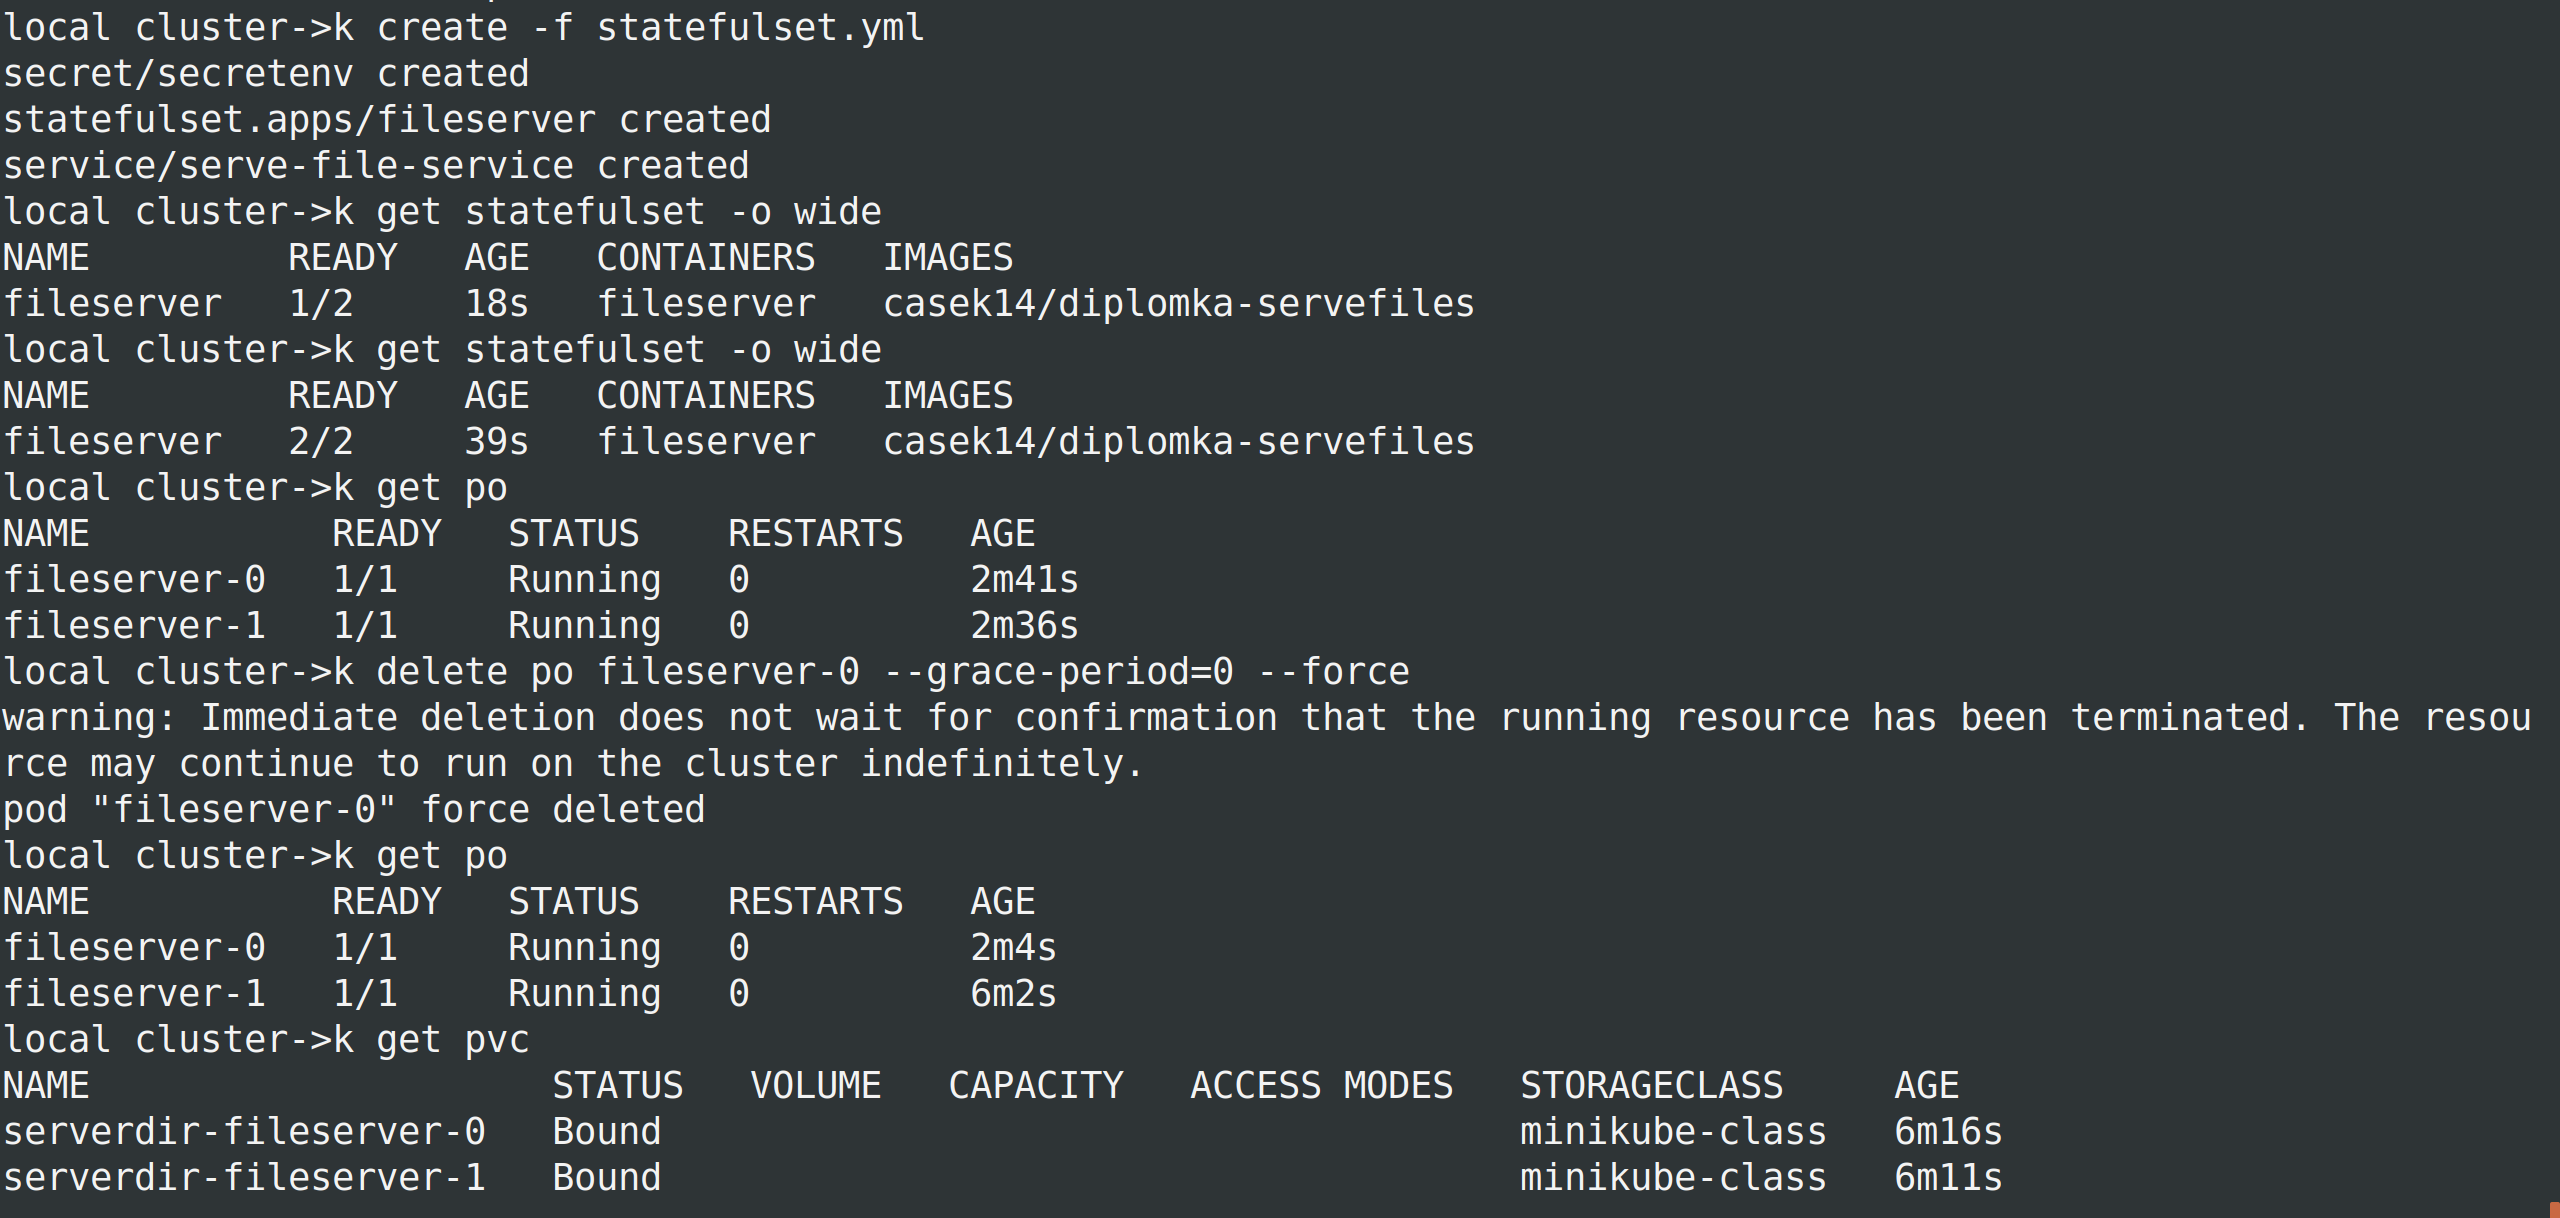
\includegraphics[width=0.9\textwidth]{images/statefulset.png}
    \par
	  \caption{Vytvoření a otestování statefulsetu\label{fig:statefulset}, zdroj: vlastní tvorba}
    \end{centering}
\end{figure}


\begin{figure}[H]
  \begin{centering}
	  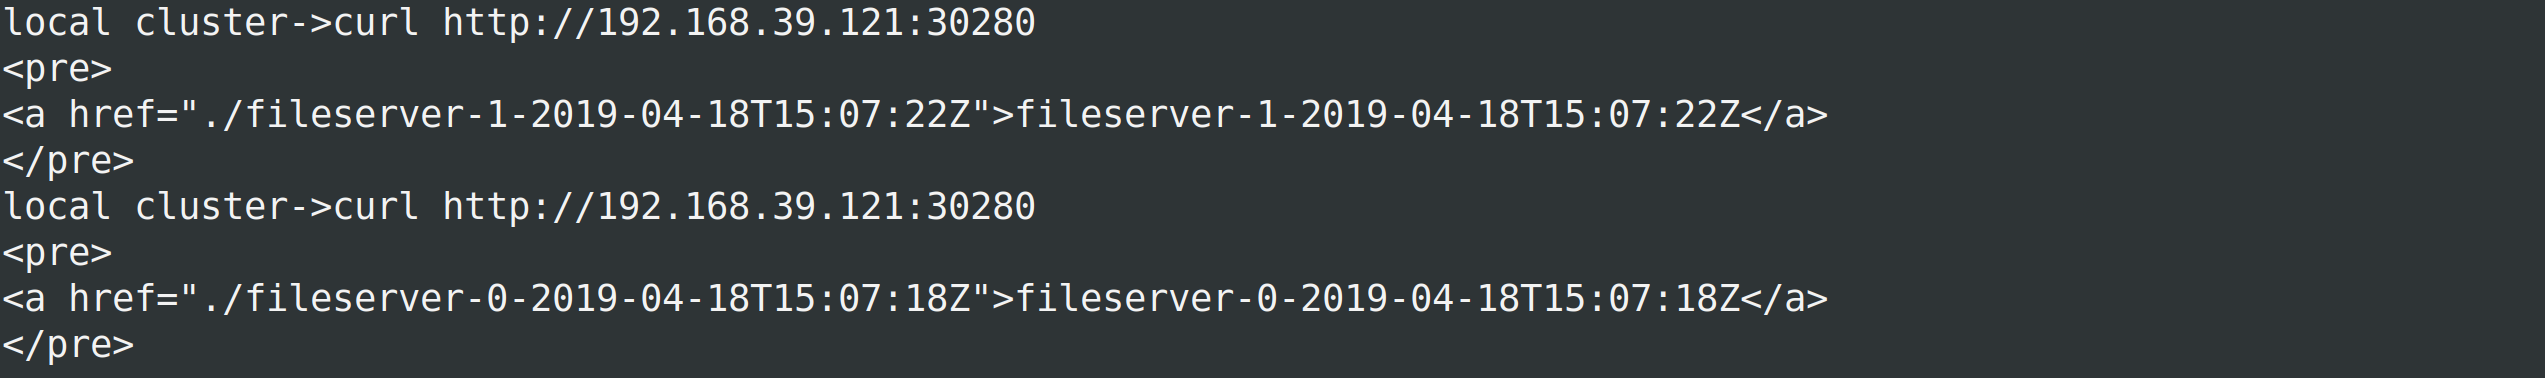
\includegraphics[width=0.9\textwidth]{images/curl1.png}
    \par
	  \caption{Data statelful aplikace\label{fig:curl1}, zdroj: vlastní tvorba}
    \end{centering}
\end{figure}

\begin{figure}[H]
  \begin{centering}
	  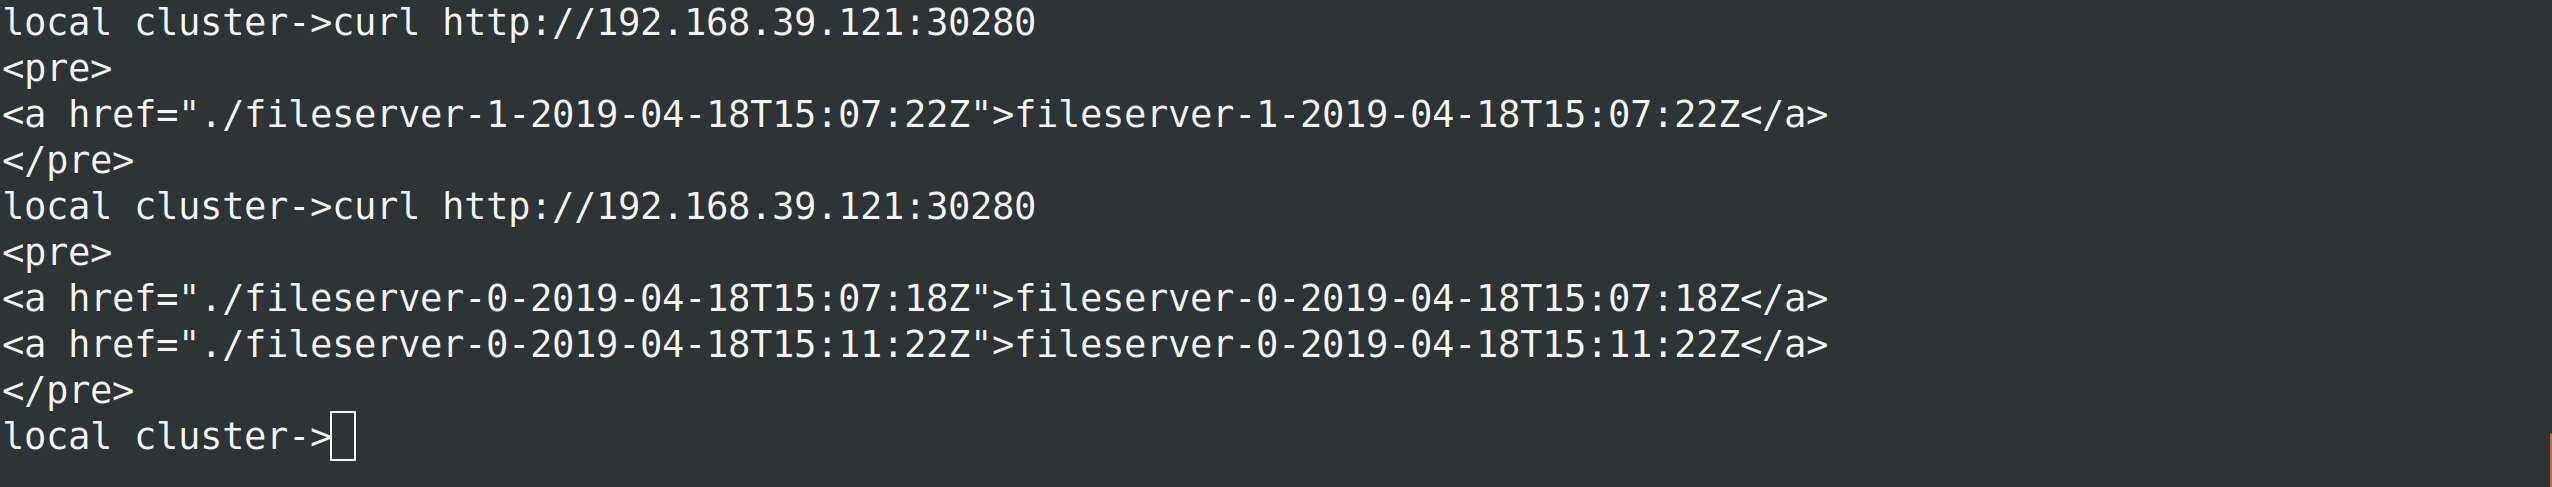
\includegraphics[width=0.9\textwidth]{images/curl2.png}
    \par
	  \caption{Data stateful aplikace po restartu jednoho z podů\label{fig:curl2}, zdroj: vlastní tvorba}
    \end{centering}
\end{figure}

\chapter{Závěry a doporučení}
Cílem práce bylo analyzovat prostředí multi-cloud technologií a řešení, a následně navrhnout platformu, která bude umožňovat běh distribuovaných aplikací v prostředí multi-cloudu. Jak ukázala rešerše cloud prostředí, moderní cloud native prostředí využívá principů mikroslužeb, které rozdělují aplikace do menší autonomních částí. Tyto části se lépe testují, spravují, škálují a umožnují tak společnostem rychleji dodávat změny. Jednotlivé mikroslužby jsou doručovány jako kontejnery. Kontejnery umožnují přenositelnost aplikací mezi prostředími, protože závislostí aplikací jsou zabaleny \linebreak s aplikací v kontejneru. Součástí cloud native přistupu jsou orchestrátory kontejnerů, které zjednodušují a automatizují správu kontejnerů. Ačkoliv na poli orchestrátorů existuje několik řešení, nejpoužívanějším orchestrátorem je Kubernetes, které se stalo synonymem pro orchestraci kontejnerů. K8s je velice dobrý nástroj, ovšem pro využití v multi-cloud prostředí je potřebné mít další nástroje, protože k8s se stará o správu pouze jednoho clusteru. Na trhu existují nástroje, které nabízí jednotnou správu zdrojů napříč public cloudem, private cloudem a fyzickými servery. Projekt, který se zaměřuje na správu více k8s clusterů Kubernetes Federated, vytváří control plane pro centrální správu několika k8s clusterů.\par
    Nabyté teoretické poznatky byly použity pro vytvoření architektury, která splňuje základní požadavky na správu více k8s clusterů. Pro vytvoření platformy je použita část architektury k8s, inspirována Kubernetes Federated projektem. Uživatelé \linebreak interagují s virtuálním k8s API, které přijímá požadavky a ukládá je do Etcd databáze a funguje jako control plane. Toto centrální API obsahuje konfigurace aplikací, které mají být spuštěny ve vybraných clusterech. Distribuci těchto konfigurací do clusterů zajišťuje vk8s manager. Vk8s manager je aplikace vytvořená v jazyce Golang, stejně jako samotné k8s. \par
        V rámci testování aplikace byly ověřeny operace a techniky, které k8s nabízí. Jako první byla testována distribuce nodů. Node je server na kterém jsou spouštěny uživatelské aplikace. Aplikace byla schopná synchronizovat nody z plnohodnotného k8s clusteru do centrálního API. Uživatelé tak mohou dohledat informace o názvech nodů, verzích komponent a také běhové prostředí kontejnerů, které daný node využívá. \linebreak Druhým testovaným scénářem byla distribuce podů, které jsou základním k8s zdrojem. V tomto případě bylo ověřeno, že pody vytvořené v centrálním API jsou podle konfigurace spuštěny k8s clusteru. Aplikace tento úkol bez problémů zvládla. Pod byl úspěnšně spuštěn, vykonal svou úlohu, která spočívala ve vypsání jednoduché hlášky, a poté byl ukončen. Všechny potřebné informace pro uživatele byly opět zapsány do centrálního API. Třetím testovaným případem byla práce s deploymenty. Distribuce a spuštění deploymentu v k8s clusteru fungovalo podle představ. Deployment byl spuštěn v minikube k8s clusteru a byl dostupný pro uživatele zvenčí s využitím dalšího k8s zdroje servicy. Další funkcí deploymentu je možnost změnit verzi aplikace. Vytvářená aplikace zvládla změnu verze z v1 na verzi v2, která byla dále změněna \linebreak na verzi v3. Verze v3 ovšem obsahovala chybu a tak byla pomocí nástroje “rollout” vrácena zpět na funkční verzi v2. Dalším testem bylo škálování aplikace, kterou testovaná aplikace zvládla. Nově vytvořené pody se ihned po nastartování zapojily \linebreak do vyřizování uživatelských požadavků. Posledním testovaným scénařem byl statefulset. V rámci testu byly vytvořeny dva pody, každý s trvalým uožištěm pro soubory s kterými pracuje. Následně byl jeden pod smazán. Vytvořená data byla přístupná v nově vytvořeném podu podle předpokladů. Data aplikace nebyla poškozená a výpadek funkčnosti aplikace nebyl zaznamenán.\par
	    Aplikace pro distribuci konfigurací v testovaných scénářích obstála. Ve všech případech došlo k úspěšnému vytvoření zdrojů v minikube k8s clusteru, podle \linebreak konfigurace zapsané v customer k8s API. Základní informace o zdrojích v minikube clusteru byly správně distribuovány do centrálního API, kde si je uživatelé mohli \linebreak prohlížet. Během testování občas docházelo k chybnému zobrazování běžících zdrojů v centrálním API, ačkoliv byly dostupné a v minikube clusteru spuštěné. 



\addcontentsline{toc}{chapter}{Literatura} 
\addcontentsline{toc}{chapter}{Přílohy} 

\cleardoublepage{}

\begin{thebibliography}{10}
	
\end{thebibliography}

\nocite{*}
\listoffigures
\listoftables
\lstlistoflistings
\appendix
\pagenumbering{Roman}
\chapter*{Přílohy}

\section*{A. Zdrojový kód aplikace zobrazující hostname\label{app:hostname}}
\begin{verbatim}
package main

import (
        "fmt"
        "log"
        "net/http"
        "os"
       )

func handler(w http.ResponseWriter, r *http.Request) {
        name, err := os.Hostname()
        if err != nil{
                log.Println("Unable to retrieve hostname")
        }
        fmt.Fprintf(w, "HOSTNAME: %s",name)
}

func main() {
        http.HandleFunc("/",handler)
        log.Fatal(http.ListenAndServe(":80",nil))
}
\end{verbatim}


\clearpage
\section*{B. Zdrojový kód aplikace zobrazující soubory v definovaném adresáři\label{app:servefiles}}
\begin{verbatim}
package main

import (
	"log"
	"net/http"
	"os"
	"time"
)

const directoryToServe = "/tmp"

func main() {
	path := os.Getenv("DIRECTORY_PATH")
	if path == ""{
		path = directoryToServe
	}
	log.Printf("Serving directory %s",path)
	hostname, err := os.Hostname()
	if err != nil{
		log.Printf("Cannot get hostname")
	}
	time := time.Now().Format(time.RFC3339)
	fileName := path+"/"+hostname+"-"+time
	newFile,err := os.Create(fileName)
	if err != nil {
		log.Printf("unable to create a file, %s",err)
	}
	log.Printf("New file created: %s", newFile.Name())

	fs := http.FileServer(http.Dir(path))
	http.Handle("/", fs)
	log.Println("Serving files on port 3000")
	http.ListenAndServe(":3000", nil)
}
\end{verbatim}


\clearpage
\section*{C. Manifest pro vytvoření statefulsetu\label{app:statefulset}}
\begin{verbatim}
apiVersion: v1
kind: Secret
metadata:
 name: secretenv
type: Opaque
data:
  dirpath: L2RpcGxvbWthLXNlcnZlLWZpbGVz
---
apiVersion: apps/v1
kind: StatefulSet
metadata:
  name: fileserver
spec:
  serviceName: "fileserver-service"
  replicas: 2
  selector:
    matchLabels:
      app: fileserver
  template:
    metadata:
      labels:
        app: fileserver
    spec:
      containers:
      - name: fileserver
        image: casek14/diplomka-servefiles
        ports:
        - containerPort: 3000
          name: servefiles
        volumeMounts:
        - name: serverdir
          mountPath: /diplomka-serve-files
        env:
        - name: DIRECTORY_PATH
          valueFrom:
            secretKeyRef:
              name: secretenv
              key: dirpath
  volumeClaimTemplates:
  - metadata:
      name: serverdir
    spec:
      accessModes: [ "ReadWriteOnce" ]
      storageClassName: "minikube-class"
      resources:
        requests:
          storage: 1Gi
---
apiVersion: v1
kind: Service
metadata:
  name: serve-file-service
spec:
  selector:
    app: fileserver
  type: NodePort
  ports:        
  - protocol: TCP
    port: 8080
    targetPort: 3000
\end{verbatim}

\clearpage
\section*{D. Struktura aplikace\label{app:struktura}}
\begin{figure}[H]
  %\begin{centering}
    
	  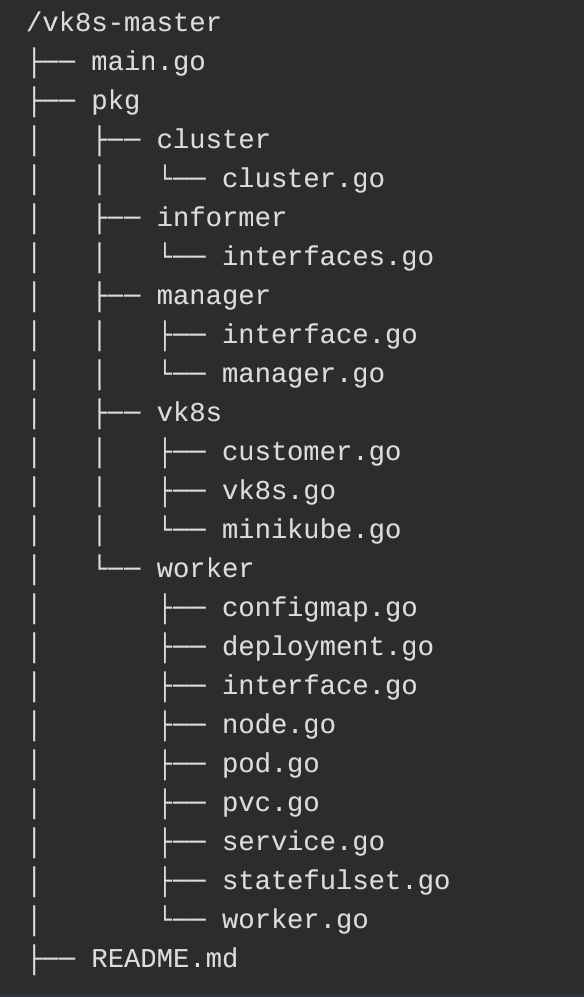
\includegraphics[width=0.5\textwidth]{images/vk8s-master.png}
   %\end{centering}
\end{figure}
%\begin{lstlistin}
%/vk8s-master\newline
%|---main.go\newline
%|---pkg\newline
%|   |---cluster\newline
%|   |   '---cluster.go\newline
%|   |---informer\newline
%|   |   '---interfaces.go\newline
%|   |---manager\newline
%|   |   |---interface.go\newline
%|   |   '---manager.go\newline
%|   |---vk8s\newline
%|   |   |---customer.go\newline
%|   |   |---vk8s.go\newline
%|   |   '---minikube.go\newline
%|   '---worker\newline
%|       |---configmap.go\newline
%|       |---deployment.go\newline
%|       |---interface.go\newline
%|       |---node.go\newline
%|       |---pod.go\newline
%|       |---pvc.go\newline
%|       |---service.go\newline
%|       |---statefulset.go\newline
%|       '---worker.go\newline
%|---README.md
%
%\end{lstlisting}


%zadani
%\includepdf[pages={1},scale=0.8]{zadani2}
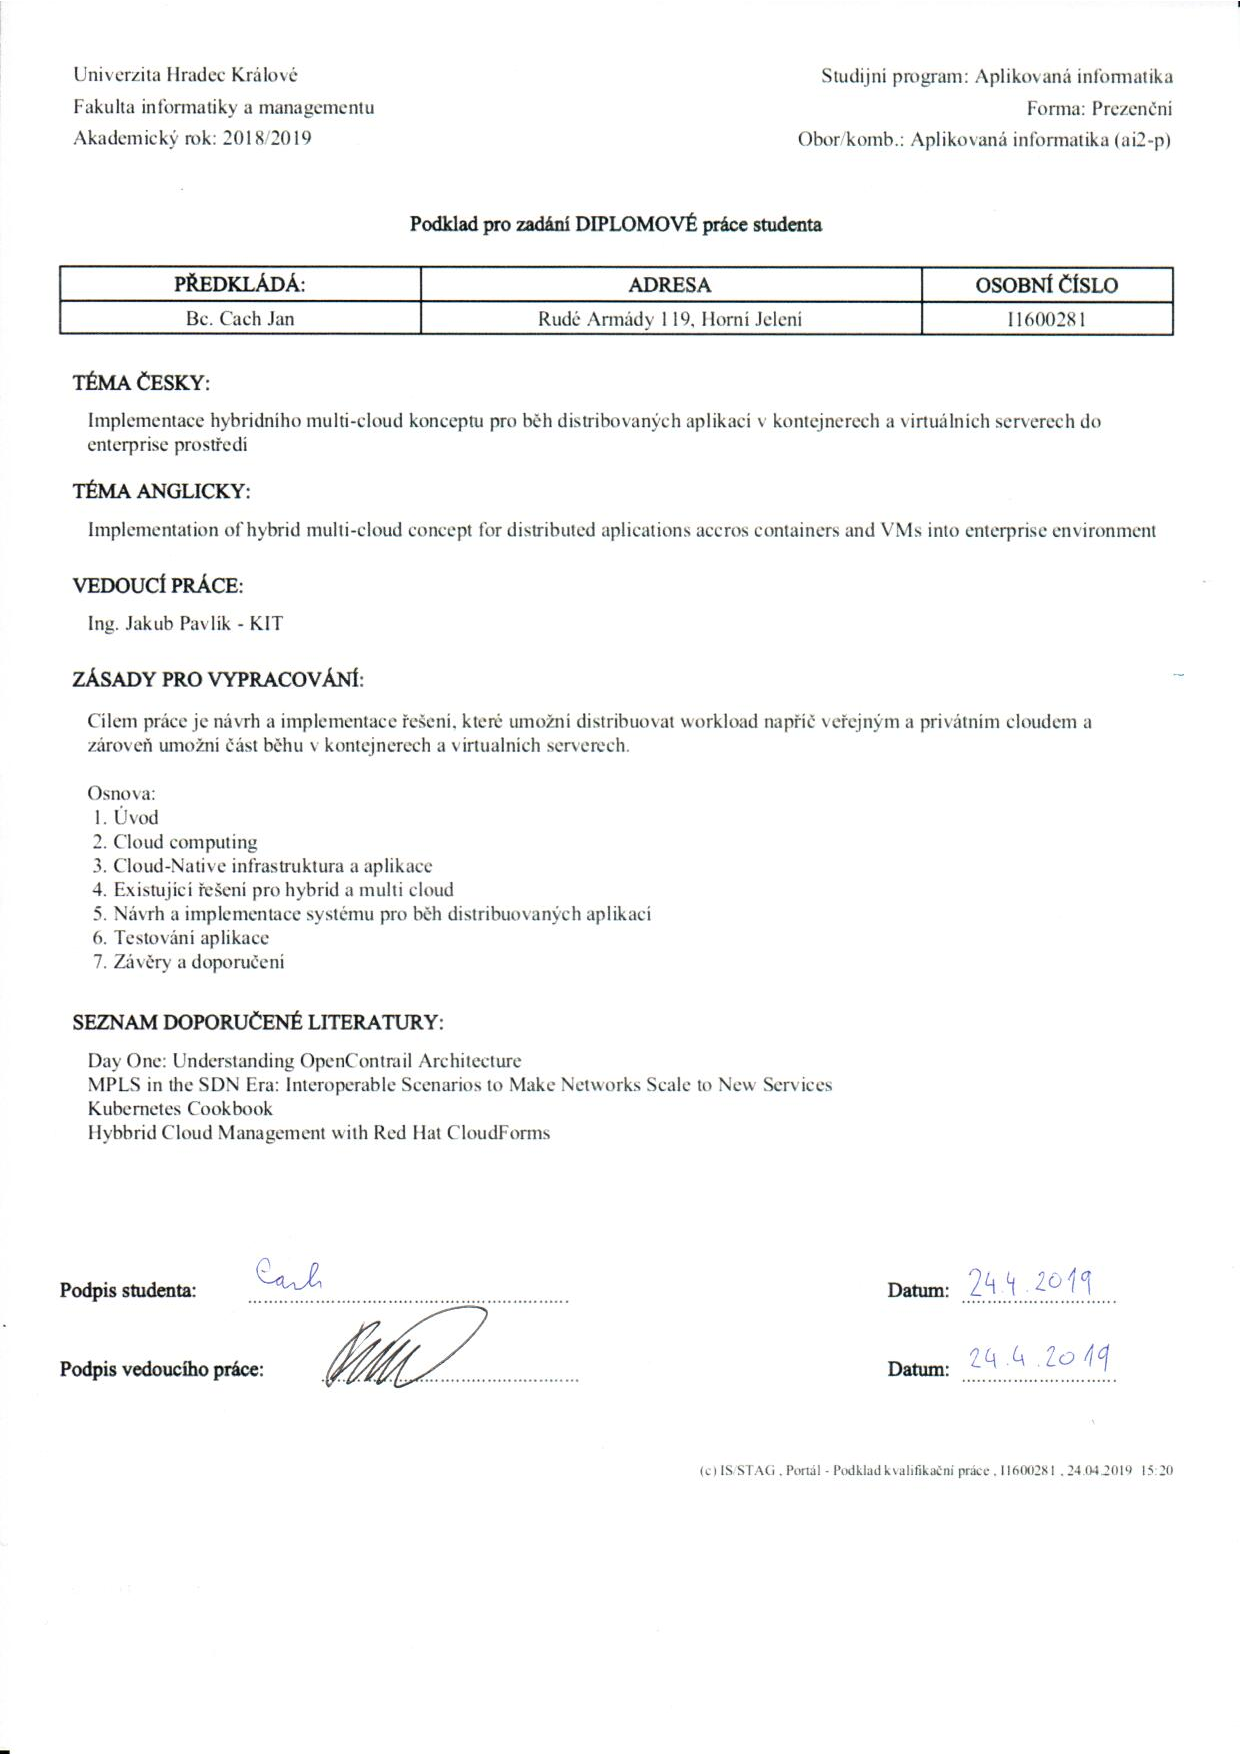
\includepdf[pages={1},scale=0.9]{images/zadani.pdf}

\clearpage{}
\end{document}
